\section{The fit model}
Fits to data, as part of the statistical analysis, are performed under the background-only and signal-plus-background hypotheses.
The fit model is completely specified by the discriminating variable used to build template distributions for signal and backgrounds  in each fitted region, and by the list of systematic uncertainties considered and their assumed correlations across regions and for the various templates. The $m_{\rm eff}$ distribution is used in all regions considered in this search. The regions with $\ge$6 jets ($\ge$7 jets) are used to perform the actual search in the 1-lepton (0-lepton) channel, whereas the regions with exactly 5 jets (6 jets) are used to validate the background modelling in different regimes of event kinematics and heavy-flavour content. A total of eight search regions and six validation regions are considered in the 1-lepton channel, whereas twelve search regions and nine validation regions are considered in the 0-lepton channel, defined in tables \ref{tab:VLQ:fit:channels1L} and \ref{tab:VLQ:fit:channels0L} respectively.
\begin{table}[t!]\footnotesize
\begin{center}
\begin{tabular}{cccc l}
\toprule\toprule
\multicolumn{5}{c}{Search regions ($\geq$6 jets)} \\     
\midrule
Mass-tagged jet multiplicity & $b$-jet multiplicity  & $m_{bb}^{min\Delta R}$ & $m_{\rm eff}$  & Channel name \\
\midrule
0 & 3 & - & $>400$ $\gev$ & 0J, $\geq$6j, 3b \\
0 & $\geq$4 & - & $>400$ $\gev$ & 0J, $\geq$6j, $\geq$4b \\     
1 & 3 & $<100$ $\gev$ & $>700$ $\gev$ & 1J, $\geq$6j, 3b, LM \\
1 & 3 & $>100$ $\gev$ & $>700$ $\gev$ & 1J, $\geq$6j, 3b, HM \\
1 & $\geq$4 & $<100$ $\gev$ & $>700$ $\gev$ & 1J, $\geq$6j, $\geq$4b, LM \\ 
1 & $\geq$4 & $>100$ $\gev$ & $>700$ $\gev$ & 1J, $\geq$6j, $\geq$4b, HM \\         
$\geq$2 & 3 & - & - & $\geq$2J, $\geq$6j, 3b \\
$\geq$2 & $\geq$4 & - & - & $\geq$2J, $\geq$6j, $\geq$4b \\     
\midrule\midrule
\multicolumn{5}{c}{Validation regions (5 jets)} \\     
\midrule
Mass-tagged jet multiplicity & $b$-jet multiplicity  & $m_{bb}^{min\Delta R}$ & $m_{\rm eff}$ & Channel name \\
\midrule
0 & 3 & - & $>400$ $\gev$ & 0J, 5j, 3b \\
0 & $\geq$4 & - & $>400$ $\gev$ & 0J, 5j, $\geq$4b \\     
1 & 3 & - & $>700$ $\gev$ & 1J, 5j, 3b \\
1 & $\geq$4 & - & $>700$ $\gev$ & 1J, 5j, $\geq$4b \\         
$\geq$2 & 3 & - & - & $\geq$2J, 5j, 3b \\
$\geq$2 & $\geq$4 & - & - & $\geq$2J, 5j, $\geq$4b \\     
\bottomrule\bottomrule
\end{tabular}
\captionsetup{width=0.85\textwidth} \caption{\small{Definition of the search and validation regions in the 1-lepton channel.}}
\label{tab:VLQ:fit:channels1L}
\end{center}
\end{table}

\begin{table}[htb!]\footnotesize
\begin{center}
\begin{tabular}{ccc l}
\toprule\toprule
\multicolumn{4}{c}{Search regions ($\geq$7 jets)} \\     
\midrule\midrule
Mass-tagged jet multiplicity & $b$-jet multiplicity  & $m_{T,{\rm min}}^{b}$ & Channel name \\
\midrule
0 & 2 & - & 0J, $\geq$7j, 2b \\
0 & 3 & - & 0J, $\geq$7j, 3b \\
0 & $\geq$4 & - & 0J, $\geq$7j, $\geq$4b \\     
1 & 2 & - & 1J, $\geq$7j, 2b \\
1 & 3 & $<160$ $\gev$ & 1J, $\geq$7j, 3b, LM \\
1 & 3 & $>160$ $\gev$ & 1J, $\geq$7j, 3b, HM \\
1 & $\geq$4 & $<160$ $\gev$ & 1J, $\geq$7j, $\geq$4b, LM \\ 
1 & $\geq$4 & $>160$ $\gev$ & 1J, $\geq$7j, $\geq$4b, HM \\         
$\geq$2 & 2 & - & $\geq$2J, $\geq$7j, 2b \\
$\geq$2 & 3 & $<160$ $\gev$ & $\geq$2J, $\geq$7j, 3b, LM \\
$\geq$2 & 3 & $>160$ $\gev$ & $\geq$2J, $\geq$7j, 3b, HM \\
$\geq$2 & $\geq$4 & - & $\geq$2J, $\geq$7j, $\geq$4b \\     
\midrule\midrule
\multicolumn{4}{c}{Validation regions (6 jets)} \\     
\midrule
Mass-tagged jet multiplicity & $b$-jet multiplicity  & $m_{T,{\rm min}}^{b}$ & Channel name \\
\midrule
0 & 2 & - & 0J, 6j, 2b \\
0 & 3 & - & 0J, 6j, 3b \\
0 & $\geq$4 & - & 0J, 6j, $\geq$4b \\     
1 & 2 & - & 1J, 6j, 2b \\
1 & 3 & - & 1J, 6j, 3b \\
1 & $\geq$4 & - & 1J, 6j, $\geq$4b \\         
$\geq$2 & 2 & - & $\geq$2J, 6j, 2b \\
$\geq$2 & 3 & - & $\geq$2J, 6j, 3b \\
$\geq$2 & $\geq$4 & - & $\geq$2J, 6j, $\geq$4b \\     
\bottomrule\bottomrule
\end{tabular}
\captionsetup{width=0.85\textwidth} \caption{\small{Definition of the search and validation regions in the 0-lepton channel.}}
\label{tab:VLQ:fit:channels0L}
\end{center}
\end{table}
Figures \ref{sec:vlq:fig:SB1l} and \ref{sec:vlq:fig:SB0l} show the expected $S/B$ and $S/\sqrt{B}$ (where $S$ and $B$ are the expected signal and background yields respectively) for 1-lepton regions and 0-lepton regions respectively assuming as signal $T\bar{T}$ production in the weak-isospin doublet and $m_{T} = 0.8$ \tev.

\begin{figure}[p]
\centering
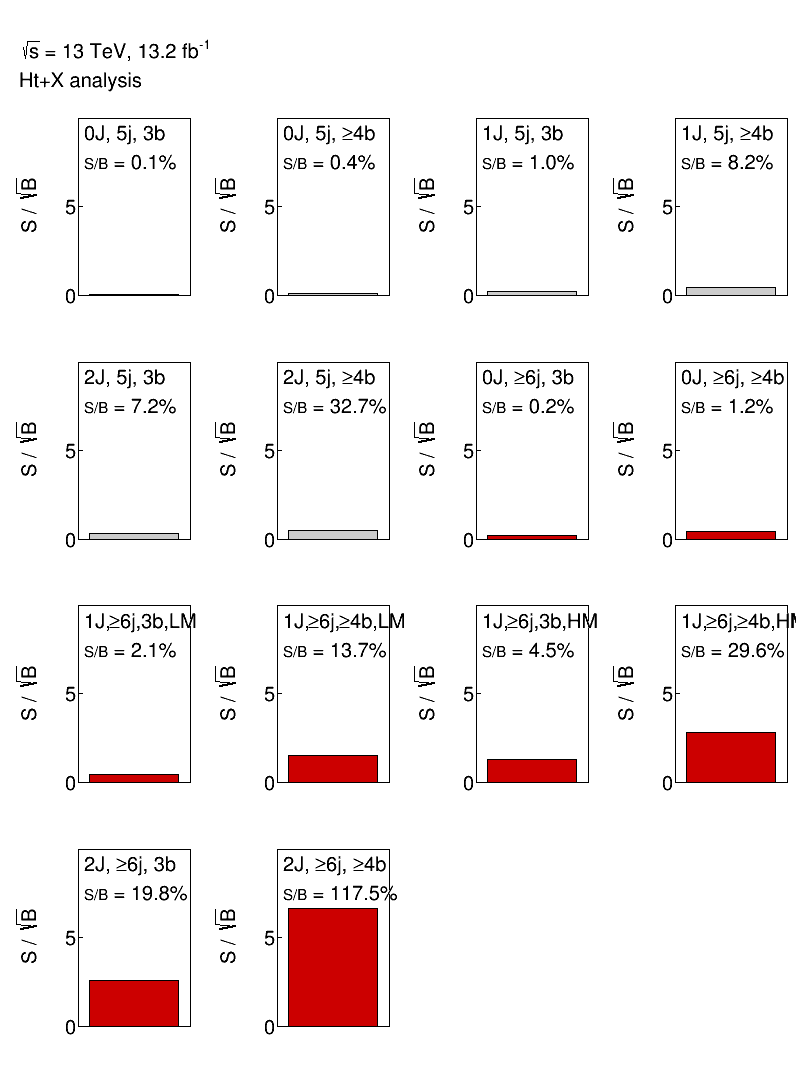
\includegraphics[width=0.4\textwidth]{figures/VLQ/SignalRegions_1L.png}
\captionsetup{width=0.85\textwidth} \caption{\small $S/B$ and $S/\sqrt{B}$ in the 1-lepton regions. The search (validation) regions are highlighted in red (grey). The signal assumed is $T\bar{T}$ production in the weak-isospin doublet and $m_{T} = 0.8$ \tev.}
\label{sec:vlq:fig:SB1l}
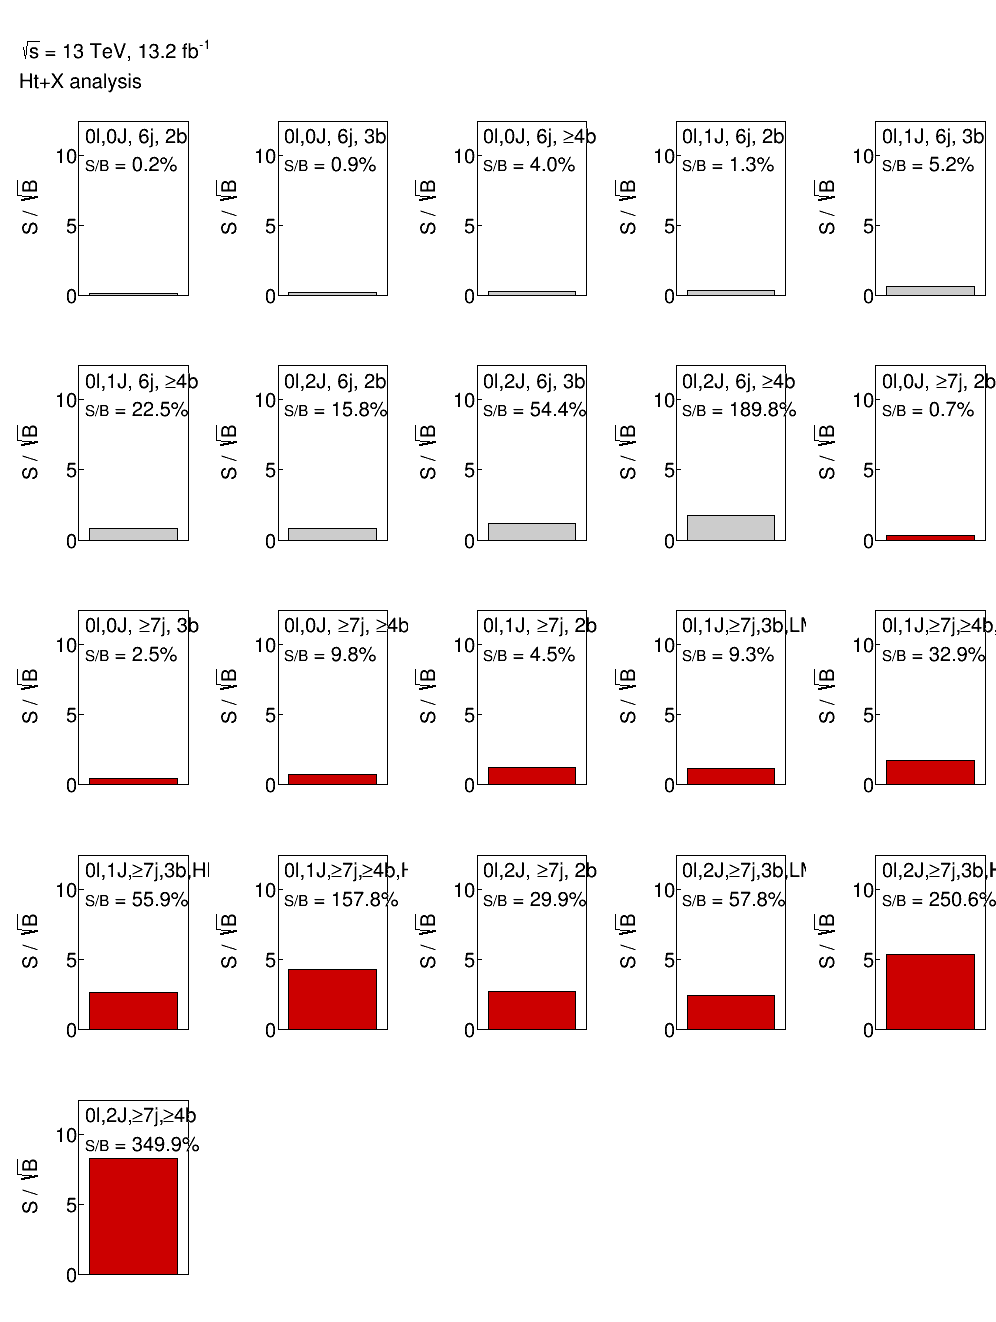
\includegraphics[width=0.5\textwidth]{figures/VLQ/SignalRegions_0L.png}
\captionsetup{width=0.85\textwidth} \caption{\small $S/B$ and $S/\sqrt{B}$ in the 0-lepton regions. The search (validation) regions are highlighted in red (grey). The signal assumed is $T\bar{T}$ production in the weak-isospin doublet and $m_{T} = 0.8$ \tev.}
\label{sec:vlq:fig:SB0l}
\end{figure}

The signal strength is considered as a free-floating parameter in the fit. The normalisation of background can be controlled through:

\bi
\ib specific nuisance parameters that implement the theoretical knowledge of the respective cross section or the uncertainty on the data-driven estimates, or
\ib free-floating normalisation parameters, whenever data is used directly to normalise a background without assuming prior knowledge.
\ei

Additional nuisance parameters associated with the rest of systematic uncertainties can impact the acceptance for each sample, the distribution of events among the analysis regions, and the shape of the discriminant distributions.
Sources of systematic uncertainties include the finite precision of the calibration of the reconstructed objects, uncertainties affecting the modelling of signal and backgrounds, and the inaccuracies in the description of the experimental conditions, e.g. luminosity or pileup.
Additional nuisance parameters associated with the finite MC statistics used to build the templates are considered only for bins for which the relative statistical uncertainty is larger than $5\%$.
Individual sources of systematic uncertainty are considered uncorrelated. Table \ref{chp:vlq:tab:SystSummary} presents a summary of the systematic uncertainties considered in the analysis, indicating if they affect the normalisation (``N'') and shape (``S'') of the templates. The table also indicates the number of specific components for systematic uncertainty. The breakdown into components is particularly desirable in the implementation of the profile likelihood fit since it results in a more flexible model, it allows to decouple the effect of each uncertainty better and to treat them as initially uncorrelated. It also helps preventing false over-constraints in some of largest systematic uncertainties due to an over-simplified treatment.\par

\begin{table}[htb!]
\centering
\begin{tabular}{lcc}
\toprule\toprule
Systematic uncertainty & Type  & Components \\
\midrule
Luminosity                  &  N & 1\\\midrule\midrule
{\bf Reconstructed Objects}                 &   & \\
Electron trigger+reco+ID+isolation              & SN & 5 \\
Electron energy scale+resolution & SN & 2 \\
Muon trigger+reco+ID+isolation                    &  SN & 6 \\
Muon momentum scale+resolution & SN & 3 \\ \midrule
Pileup reweighting         & SN    & 1\\
Jet vertex tagger         & SN    & 1\\
Jet energy scale            & SN & 18\\
Jet energy resolution       & SN & 1\\
Missing transverse momentum  & SN & 3\\ \midrule
$b$-tagging efficiency      & SN & 5\\
$c$-tagging efficiency      & SN & 4\\
Light-jet tagging efficiency    & SN & 14\\ \midrule
$b$-tagging extrapolation & SN & 2 \\ \midrule
{\bf Background Model}                 &   & \\
$t\bar{t}$ cross section    &  N & 1\\
$t\bar{t}$+HF: normalisation & N & 2 \\
$t\bar{t}$+$\geq1b$: NLO Shape & SN & 10 \\
$t\bar{t}$ modelling: Radiation & SN & 3\\
$t\bar{t}$ modelling: Generator & SN & 3\\
$t\bar{t}$ modelling: Parton shower+hadronisation & SN & 3 \\
$t\bar{t}$ NNLO reweighting  & SN & 2\\ \midrule
$V$+jets normalisation      &  N & 18\\
Single top normalisation    &  N & 6\\
Diboson normalisation  &  N & 6\\
$t\bar{t}V$ cross section   &  N & 2\\
$t\bar{t}H$ cross section & N & 2 \\
SM $t\bar{t}t\bar{t}$ cross section & N & 2 \\
Multijet normalisation  &  N & 1\\
\bottomrule\bottomrule
\end{tabular}
\captionsetup{width=0.85\textwidth}  \caption{\small List of systematic uncertainties considered. An ``N'' means that the uncertainty is taken as normalisation-only for all 
processes and channels affected, whereas ``SN" means that the uncertainty is taken on both shape and normalisation. Some of the systematic uncertainties are split into several components for a more accurate treatment.}
\label{chp:vlq:tab:SystSummary}
\end{table}

\begin{figure}[p]
\centering
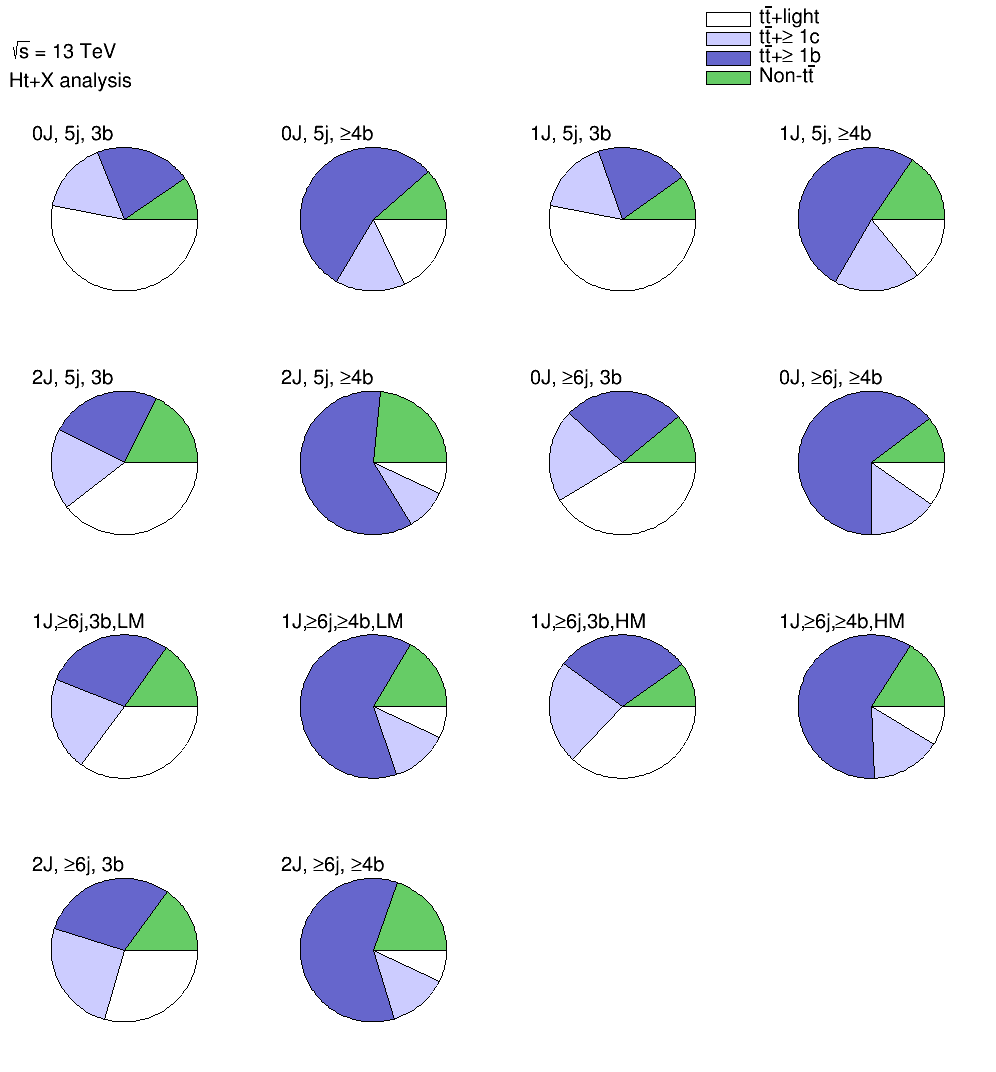
\includegraphics[width=0.4\textwidth]{figures/VLQ/PieChart_1L.png}
\captionsetup{width=0.85\textwidth} \caption{\small Fractional contribution of the various backgrounds to the total background prediction in the different 1-lepton regions. The small contributions from $t\bar{t} V$, $t\bar{t} H$, single top, $W/Z$+jets, diboson, and multijet backgrounds are combined into a single background source referred to as ``Non-$t\bar{t}$''.}
\label{sec:vlq:fig:Pie1l}
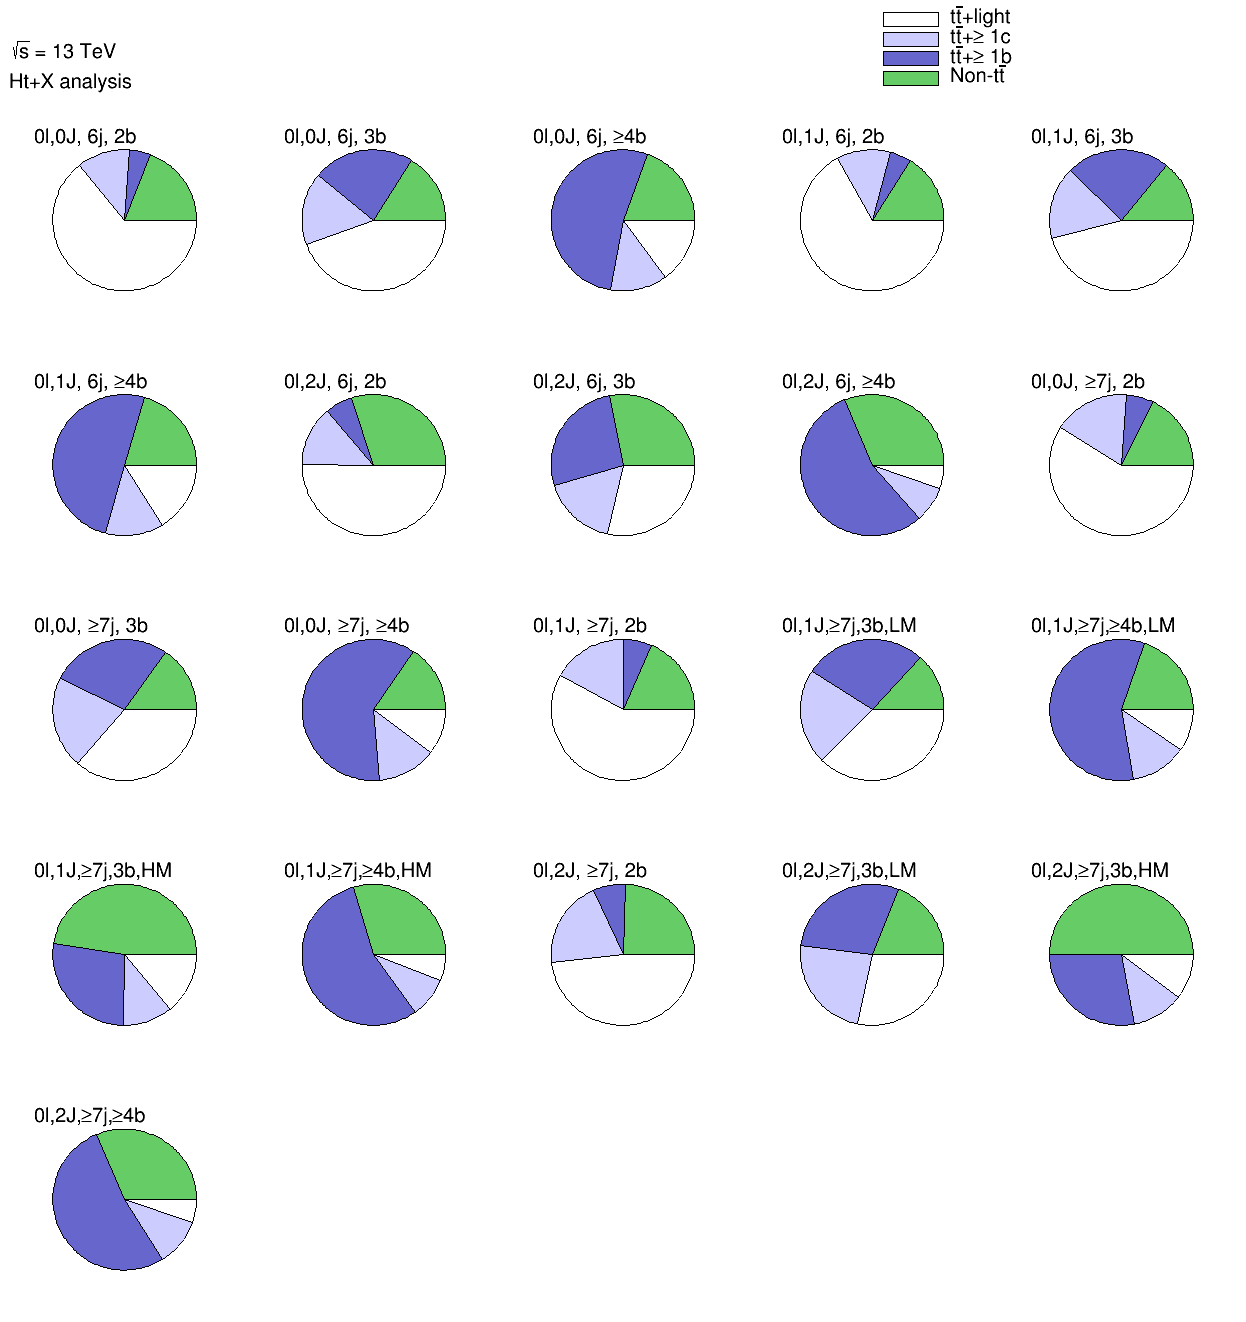
\includegraphics[width=0.5\textwidth]{figures/VLQ/PieChart_0L.png}
\captionsetup{width=0.85\textwidth}  \caption{\small Fractional contribution of the various backgrounds to the total background prediction in the different 0-lepton regions. The small contributions from $t\bar{t} V$, $t\bar{t} H$, single top, $W/Z$+jets, diboson, and multijet backgrounds are combined into a single background source referred to as ``Non-$t\bar{t}$''.}
\label{sec:vlq:fig:Pie0l}
\end{figure}
\begin{figure}[htb!]
\centering
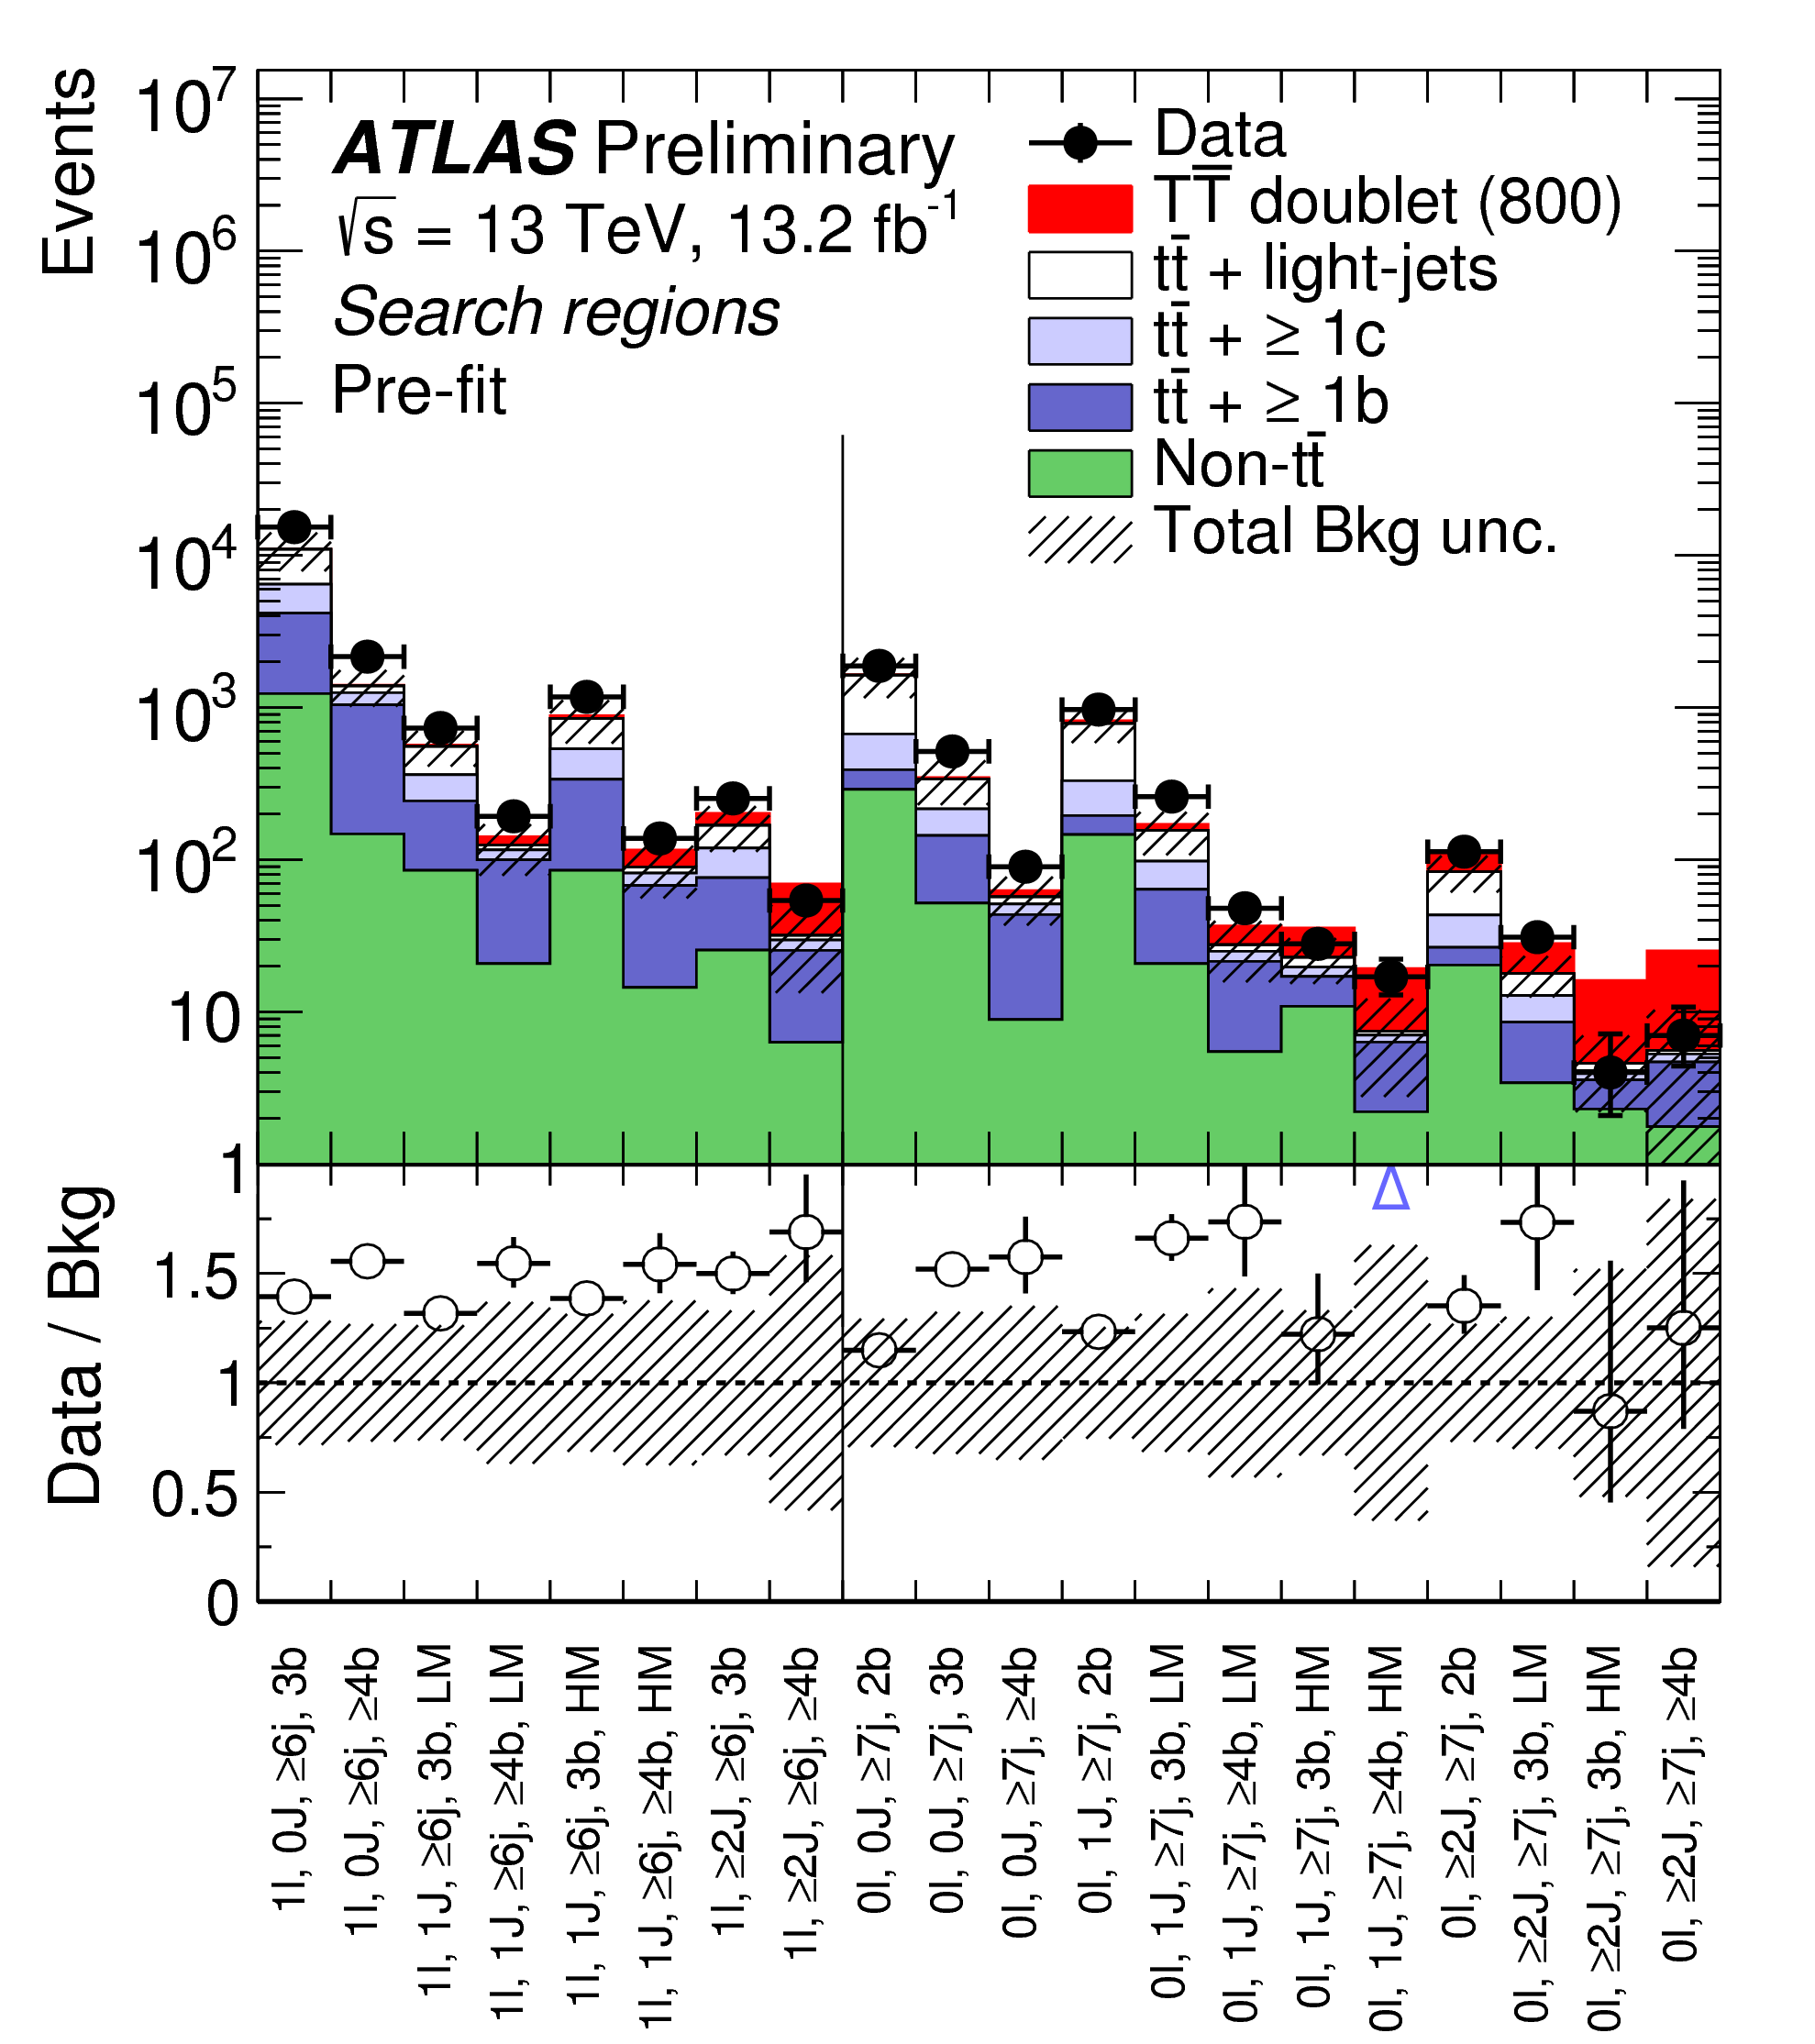
\includegraphics[width=0.5\textwidth]{figures/VLQ/fig_08.png}
\captionsetup{width=0.85\textwidth}  \caption{\small Comparison between the data and the background prediction for the yields in the search regions considered  in the 1-lepton and 0-lepton channels, before the fit to data (``Pre-fit"). The small contributions from $t\bar{t}V$, $t\bar{t}H$, single top, $W/Z$+jets, diboson, and multijet backgrounds are combined into a single background source referred to as ``Non-$t\bar{t}$''. The expected $T\bar{T}$ signal (solid red) corresponding to $m_{T}=800$ $\gev$ in the doublet $T$-quark scenario is also shown,  added on top of the background prediction. The bottom panel displays the ratio of data to the SM background (``Bkg'') prediction.  The blue triangles indicate points that are outside the vertical range of the figure. The hashed area represents the total uncertainty on the background, excluding the normalisation uncertainty on the $t\bar{t}+\ge1b$ background.}
\label{sec:vlq:fig:prefityields}
\end{figure}
The composition of the $t\bar{t}$+jets background strongly depends on the jet and $b$-tag multiplicities, as illustrated in Figure \ref{sec:vlq:fig:Pie1l} and \ref{sec:vlq:fig:Pie0l}. The $t\bar{t}$+light-jets background is dominant in events with exactly two or three $b$-tagged jets. The former typically consists of events with the two $b$-quarks from the top quark decays being tagged, while the latter is dominated by events where in addition a charm quark from the hadronic $W$-boson decay is tagged. Contributions from $t\bar{t}$+$\ge$$1c$ and $t\bar{t}$+$\ge$$1b$ backgrounds become significant as the $b$-tag multiplicity increases, with the $t\bar{t}$+$\ge$$1b$ background being dominant for events with $\ge$ 4 $b$-tagged jets. The regions with different mass-tagged jet multiplicities allow probing different kinematic regimes, both soft (e.g. low-mass $T$ quark or SM $t\bar{t}t\bar{t}$) and hard (e.g. high-mass $T$ quark or BSM $t\bar{t}t\bar{t}$).
The aim of the profiled likelihood procedure is to use the background dominated regions to improve the knowledge of the background (through constraints of nuisance parameters or creation of correlations) and extrapolate this knowledge into signal-enriched regions where a smaller uncertainty on the background predictions can lead to an improvement in sensitivity.
The search regions, with the higher multiplicities of mass-tagged jets and $b$-tagged jets, typically have the largest signal-to-background ratio, and therefore drive the sensitivity of the search. The rest of search regions have significantly lower signal-to-background ratios, but they are useful for checking and correcting the $t\bar{t}$+jets background prediction and constraining the related systematic uncertainties through the likelihood fit to data.
This is particularly important in the context of the $t\bar{t}+\ge1b$ normalisation, which is underestimated by the simulation, leading to a deficit in the prediction relative to the data that is most apparent in the channels with $\ge$4 $b$-tagged jets.
The distribution of expected and observed yields across the multiple search regions before the fit to data (``pre-fit") is shown in figure \ref{sec:vlq:fig:prefityields}.
A summary of the observed and expected yields pre-fit in four of the most sensitive search regions in the 1-lepton and 0-lepton channels can be found in tables \ref{tab:VLQ:fit:PrefitYields1Lunblind} and \ref{tab:VLQ:fit:PrefitYields0Lunblind} respectively. The search regions shown in table \ref{tab:VLQ:fit:PrefitYields1Lunblind} for the 1-lepton channel, all requiring $\ge$4 $b$-tagged jets but with different requirements on mass-tagged multiplicity, are a selection of some of the regions with the highest $S/B$ ratio across several signal benchmark scenarios considered ($T\bar{T}$ in the doublet $T$-quark scenario, $t\bar{t}t\bar{t}$  within SM and BSM, associated heavy Higgs boson production). Similarly, the search regions shown in table \ref{tab:VLQ:fit:PrefitYields0Lunblind} for the 0-lepton channel are a superset of the regions with the highest $S/B$ ratio for different $T\bar{T}$ signal benchmark scenarios (doublet $T$-quark, singlet $T$-quark and ${\rm BR}(T\to Zt) = 1$).
\begin{table}[htb!]
\begin{center}
\begin{tabular}{l*{4}{c}}
\toprule\toprule
1-lepton channel & 0J, $\geq$6j, $\geq$4b & 1J, $\geq$6j, $\geq$4b & 1J, $\geq$6j, $\geq$4b & $\geq$2J, $\geq$6j, $\geq$4b  \\
& & LM & HM & \\
\midrule\midrule
\multicolumn{5}{l}{$T\bar{T}$  ($m_{T}=1$ \tev)} \\      
{\,} ${\rm BR}(T\to Ht)=1$  & $ 3.13 \pm 0.67 $ &   $ 4.0 \pm 1.0 $ &   $ 8.7 \pm 1.6 $ &   $ 19.2 \pm 3.1 $ \\ 
{\,} $(T,B)$ or $(X,T)$ doublet & $ 2.38 \pm 0.47 $ &   $ 2.98 \pm 0.56 $ &   $ 5.04 \pm 0.94 $ &   $ 9.6 \pm 1.7 $ \\ 
{\,} $T$ Singlet  & $ 1.24 \pm 0.25 $ &   $ 1.27 \pm 0.25 $ &   $ 2.46 \pm 0.51 $ &   $ 3.83 \pm 0.73 $  \\ [0.2cm]
\multicolumn{5}{l}{$t\bar{t}t\bar{t}$} \\
{\,} EFT ($|C_{4t}|/\Lambda^2 = 4\pi$ \tev$^{-2}$) & $ 205 \pm 34 $ &   $ 105 \pm 18 $ &   $ 155 \pm 29 $ &   $ 181 \pm 34 $  \\ 
{\,} 2UED/RPP ($m_{\rm KK}=1.4$ \tev) & $ 0.31 \pm 0.09 $ &   $ 0.48 \pm 0.11 $ &   $ 2.08 \pm 0.52 $ &   $ 9.7 \pm 1.9 $ \\ [0.2cm]
\multicolumn{5}{l}{Heavy Higgs bosons ($m_{H^\pm, H}=1$ \tev, $\sigma=1$~pb)} \\
{\,} $b\bar{b}H$\ & $ 42.0 \pm 7.5 $ &   $ 23.2 \pm 4.2 $ &   $ 31.2 \pm 6.0 $ &   $ 5.3 \pm 1.3 $ \\ 
{\,} $t\bar{t}H$\ & $ 210 \pm 34 $ &   $ 162 \pm 27 $ &   $ 205 \pm 35 $ &   $ 220 \pm 38 $ \\
{\,} $tbH^{\pm}$\ & $ 90 \pm 16 $ &   $ 29.6 \pm 5.7 $ &   $ 56 \pm 11 $ &   $ 19.7 \pm 4.5 $ \\ 
\midrule\midrule
$t\bar{t}$+light-jets & $ 136 \pm 82 $ &   $ 9.0 \pm 5.3 $ &   $ 7.8 \pm 5.1 $ &   $ 2.3 \pm 1.6 $ \\ 
$t\bar{t}$+$\geq$$1c$ & $ 210 \pm 130 $ &   $ 16 \pm 10 $ &   $ 14 \pm 10 $ &   $ 4.2 \pm 3.2 $ \\ 
$t\bar{t}$+$\geq$$1b$ & $ 890 \pm 210 $ &   $ 79 \pm 38 $ &   $ 53 \pm 24 $ &   $ 19 \pm 14 $ \\  
$t\bar{t}V$ & $ 25.4 \pm 9.0 $ &   $ 4.2 \pm 1.5 $ &   $ 2.19 \pm 0.80 $ &   $ 1.21 \pm 0.44 $ \\  
$t\bar{t}H$ & $ 51 \pm 18 $ &   $ 5.7 \pm 2.0 $ &   $ 5.7 \pm 2.0 $ &   $ 2.27 \pm 0.83 $ \\ 
$W$+jets & $ 19 \pm 10 $ &   $ 3.7 \pm 2.0 $ &   $ 1.08 \pm 0.56 $ &   $ 0.56 \pm 0.32 $ \\ 
$Z$+jets & $ 4.0 \pm 2.2 $ &   $ 0.41 \pm 0.38 $ &   $ 0.11 \pm 0.07 $ &   $ 0.08 \pm 0.06 $ \\   
Single top & $ 42 \pm 15 $ &   $ 5.0 \pm 1.7 $ &   $ 4.3 \pm 1.6 $ &   $ 1.04 \pm 0.57 $ \\
Diboson & $ 3.9 \pm 2.2 $ &   $ 0.62 \pm 0.47 $ &   $ 0.06 \pm 0.19 $ &   $ 0.09 \pm 0.06 $ \\
$t\bar{t}t\bar{t}$ (SM) & $ 2.88 \pm 0.47 $ &   $ 1.04 \pm 0.18 $ &   $ 1.03 \pm 0.18 $ &   $ 1.08 \pm 0.19 $ \\ 
\midrule
Total background & $ 1390 \pm 370 $ &   $ 125 \pm 45 $ &   $ 89 \pm 31 $ &   $ 32 \pm 16 $ \\ 
\midrule
Data & 2160  & 193  & 138  & 54  \\ 
\bottomrule\bottomrule     \\
\end{tabular}

\vspace{0.1cm}

\end{center}
\vspace{-0.5cm}
\captionsetup{width=0.85\textwidth} \caption{\small Predicted and observed yields in the 1-lepton channel in four of the most-sensitive search regions (depending on the signal scenario) considered. 
The multijet background is estimated to be negligible in these regions and thus not shown. The background prediction is shown before the fit to data. Also shown are the signal predictions for different benchmark scenarios considered. The quoted uncertainties are the sum in quadrature of statistical and systematic uncertainties on the yields, excluding the normalisation uncertainty on the $t\bar{t}+\ge1b$ background.}
\label{tab:VLQ:fit:PrefitYields1Lunblind}
\end{table}
\begin{table}[htb!]
\begin{center}
\begin{tabular}{l*{4}{c}}
\toprule\toprule
0-lepton channel & 1J, $\geq$7j, $\geq$4b & 2J, $\geq$7j, $\geq$2b & $\geq$2J, $\geq$7j, 3b & $\geq$2J, $\geq$7j, $\geq$4b  \\
& HM & & HM & \\
\midrule\midrule
\multicolumn{5}{l}{$T\bar{T}$  ($m_{T}=1$ \tev)} \\      
{\,} ${\rm BR}(T\to Zt)=1$  & $ 1.58 \pm 0.42 $ &   $ 10.2 \pm 1.4 $ &   $ 2.92 \pm 0.58 $ &   $ 1.96 \pm 0.61 $ \\ 
{\,} $(T,B)$ or $(X,T)$ doublet & $ 2.44 \pm 0.50 $ &   $ 7.56 \pm 0.78 $ &   $ 3.94 \pm 0.48 $ &   $ 6.0 \pm 1.1 $ \\ 
{\,} $T$ Singlet  & $ 0.94 \pm 0.29 $ &   $ 3.98 \pm 0.41 $ &   $ 1.62 \pm 0.21 $ &   $ 2.17 \pm 0.41 $ \\  
\midrule\midrule
$t\bar{t}$+light-jets & $ 0.44 \pm 0.26 $ &   $ 40 \pm 12 $ &   $ 0.48 \pm 0.19 $ &   $ 0.30 \pm 0.18 $ \\   
$t\bar{t}$+$\geq$$1c$ & $ 0.70 \pm 0.46 $ &   $ 17 \pm 10 $ &   $ 0.54 \pm 0.33 $ &   $ 0.60 \pm 0.40 $ \\
$t\bar{t}$+$\geq$$1b$ & $ 4.1 \pm 3.0 $ &   $ 6.3 \pm 2.6 $ &   $ 1.28 \pm 0.45 $ &   $ 2.93 \pm 0.90 $ \\   
$t\bar{t}V$ & $ 0.40 \pm 0.11 $ &   $ 3.80 \pm 0.80 $ &   $ 0.40 \pm 0.10 $ &   $ 0.28 \pm 0.08 $ \\   
$t\bar{t}H$ & $ 0.46 \pm 0.11 $ &   $ 0.66 \pm 0.14 $ &   $ 0.11 \pm 0.03 $ &   $ 0.29 \pm 0.09 $ \\ 
$W$+jets & $ 0.37 \pm 0.20 $ &   $ 5.2 \pm 2.4 $ &   $ 0.32 \pm 0.16 $ &   $ 0.21 \pm 0.14 $ \\   
$Z$+jets & $ 0.32 \pm 0.22 $ &   $ 3.5 \pm 1.7 $ &   $ 0.29 \pm 0.15 $ &   $ 0.08 \pm 0.11 $ \\ 
Single top & $ 0.37 \pm 0.27 $ &   $ 4.9 \pm 3.2 $ &   $ 0.62 \pm 0.47 $ &   $ 0.21 \pm 0.19 $ \\ 
Diboson & $ 0.19 \pm 0.21 $ &   $ 2.1 \pm 1.7 $ &   $ 0.50 \pm 0.76 $ &   $ 0.48 \pm 0.49 $ \\  
$t\bar{t}t\bar{t}$ (SM) &   $ 0.10 \pm 0.04 $ &   $ 0.22 \pm 0.08 $ &   $ 0.05 \pm 0.02 $ &   $ 0.20 \pm 0.07 $ \\ 
\midrule
Total background & $ 7.5 \pm 3.5 $ &   $ 84 \pm 21 $ &   $ 4.6 \pm 1.5 $ &   $ 5.6 \pm 1.6 $ \\
\midrule
Data & 17  & 113  & 4  & 7  \\ 
\bottomrule\bottomrule     \\
\end{tabular}
\vspace{0.1cm}
\end{center}
\vspace{-0.5cm}
\captionsetup{width=0.85\textwidth} \caption{\small Predicted and observed yields in the 0-lepton channel in four of the most-sensitive search regions  (depending on the signal scenario) considered. 
The multijet background is assumed to be negligible in these regions and thus not shown. The background prediction is shown before the fit to data. Also shown are the signal predictions for different benchmark scenarios considered. The quoted uncertainties are the sum in quadrature of statistical and systematic uncertainties on the yields, excluding the normalisation uncertainty on the $t\bar{t}+\ge1b$ background. }
\label{tab:VLQ:fit:PrefitYields0Lunblind}
\end{table}
\\ \indent In the following sections, a brief description of the sources of systematic uncertainties is provided, with particular emphasis on the $t\bar{t}+$jets uncertainties. The expected fit performance and the actual fit results are also discussed. 

\subsection{Systematic uncertainties}
\label{chp:vlq:sec:syst}
\subsubsection{Luminosity}
The uncertainty on the integrated luminosity is estimated to be of $2.9\%$ at $\sqrt{s} =13$ $\tev$. This systematic uncertainty affects all processes for which the event yield from simulation is used. The multijet background is not affected by this uncertainty since it is derived from a data-driven method.

\subsubsection{Pileup}
The uncertainty is evaluated changing the rescaling of $\mu$ in the pileup reweighting procedure. 

\subsubsection{Reconstructed objects}

The object reconstruction and calibration introduces uncertainties associated with the definition of leptons, jets and \MET. The corresponding systematic uncertainties were described in chapter \ref{chp:obj} . The largest individual uncertainties affecting the background in the most-sensitive search regions are the first eigenvalues of the flavour tagging uncertainty ($b$, $c$ and mistag efficiency), jet energy scale and jet vertex tagger uncertainties. 

\subsubsection[$t\bar{t}$ modelling]{\boldmath{$t\bar{t}$} modelling}

The $t\bar{t}$ inclusive cross section is computed at NNLO+NNLL in QCD with a total uncertainty of $+5.5\%/-6.1\%$ \cite{topPP}, including effects from varying the factorisation and renormalisation scales, the PDF, $\alpha_{S}$, and the top-quark mass. In the regions where $t\bar{t}+\ge1b$ dominates, the background prediction underestimates the data, although the excess is compatible with the prediction given the large uncertainties associated with $t\bar{t}+\ge1b$ production. Therefore, the $t\bar{t}+\ge1b$ normalisation, assumed without any prior uncertainty, will be determined from data using a free floating parameter in the fit to avoid any bias. The analysis regions have little sensitivity for the $t\bar{t}+\ge1c$ normalisation, and thus the fit is unable to measure it from data. As a result, the analysis has very limited sensitivity to this uncertainty, for which a normalisation uncertainty of $50\%$ is assumed.\par
The effects of initial and final-state radiation (ISR/FSR) are explored using two alternative {\sc Powheg-Box+Pythia} samples, one with {\tt hdamp} parameter set to $2m_{t}$, the renormalisation and factorisation scales set to half the nominal value and using the P2012 radHi UE tune, giving more radiation (referred to as ``radHi''), and one with the P2012 radLo UE tune, {\tt hdamp} set to $m_{t}$ and the renormalisation and factorisation scales set to twice the nominal value, giving less radiation (referred to as ``radLow''). The uncertainties associated with the modelling of ISR/FSR are obtained from the comparison of the two alternative samples, ``radHi'' and ``radLow'',  with the nominal {\sc Powheg-Box+Pythia} sample.\par
An uncertainty associated with the choice of NLO generator is derived by comparing two $t\bar{t}$ samples, one generated with {\sc Powheg-Box+Herwig++} and another generated with {\sc MG5$\_$aMC+Herwig++}, and propagating the resulting fractional difference to the nominal {\sc Powheg-Box+Pythia} prediction.
An uncertainty due to the choice of parton shower and hadronisation model is derived by comparing events produced by {\sc Powheg-Box} interfaced to {\sc Pythia} or {\sc Herwig++}.
Finally, the uncertainty on the modelling of the top-quark $\pt$ is evaluated by taking the full difference between applying and not applying the reweighting to match the NNLO prediction.\footnote{This uncertainty only affects the $t\bar{t}+$light-jets and $t\bar{t}+\ge1c$ processes.} \par
The above uncertainties are taken as uncorrelated between the $t\bar{t}+$light-jets, $t\bar{t}+\ge1c$ and $t\bar{t}+\ge1b$ processes, except for the uncertainty on the inclusive $\ttbar$ cross section. This treatment prevents an undue reduction of these systematic uncertainties on $t\bar{t}+\ge1c$ and $t\bar{t}+\ge1b$ by constraining them for $t\bar{t}+$light-jets via the fit to data in the high-statistics channels with two $b$-tagged jets.
In the case of $t\bar{t}+\ge1b$, in all instances the various HF categories and the corresponding partonic kinematics for the alternative MC samples are reweighted to match the NLO prediction of {\sc SherpaOL}, so that only effects other than distortions to the inter-normalisation of the various $t\bar{t}+\ge1b$ topologies and their parton-level kinematics are propagated.
In the case of $t\bar{t}$+light-jets and $t\bar{t}+\ge1c$, the full effect of these uncertainties is propagated. 
Similarly to the treatment of the NLO corrections and uncertainties on $t\bar{t}+\ge1b$  discussed above, in the case of the additional uncertainties derived by comparing alternative $t\bar{t}$ samples, the overall normalisation of the $t\bar{t}+\ge1b$  and $t\bar{t}+\ge1c$ background at the particle level is fixed to the nominal prediction. In this way, only migrations across categories and distortions to the shape of the kinematic distributions are considered. In order to maintain the inclusive $t\bar{t}$ cross section, the $t\bar{t}$+light-jets background is adjusted accordingly. These uncertainties  are referred to as ``$\ttbar$+$\ge1b$ residual uncertainties''.
This approach gives to the $t\bar{t}+\ge1b$  and $t\bar{t}+\ge1c$  normalisation NPs the meaning of scale factors to the cross section at particle level for these two processes. \par
Finally, uncertainties on the SherpaOL NLO prediction, which is used for reweighting the nominal {\sc Powheg-Box+Pythia}  $t\bar{t}+\ge1b$ prediction, are considered. They are evaluated by varying the renormalisation scale up and down by a factor of two and as well as using two different scale variations (see table \ref{chp:vlq:tab:sherpascales}), a different shower-recoil model scheme, and two alternative PDF sets (MSTW and NNPDF), and they affect both shape and intercategory migration effects in $t\bar{t}+\ge1b$ production.
An uncertainty associated on the choice of NLO generator is derived by comparing the $t\bar{t}+\ge1b$ predictions obtained after reweighting {\sc Powheg-Box+Pythia} to the NLO calculation from {\sc SherpaOL} and to an equivalent NLO calculation from {\sc MG5$\_$aMC+Pythia8}. The uncertainty from the parton shower and hadronisation model is taken from the difference between the {\sc MG5$\_$aMC} calculation showered with either {\sc Pythia8} or {\sc Herwig++}.
These uncertainties are referred to as ``$t\bar{t}+\ge1b$ reweighting uncertainties''.
Additional uncertainties are assessed for the contributions to the $t\bar{t}+\ge1b$  background originating from MPI or FSR from top-quark decay products, which are not part of the NLO prediction. The MPI uncertainty is assumed to be $50\%$ based on studies of different underlying event tunes while the FSR uncertainty is assessed via the alternative ``radHi'' and ``radLow'' samples.


\begin{table}
\begin{center}
\begin{tabular}{lccc}
\hline\hline
Scale & default & glosoft & Q-CMMPS \\
\hline
$\mu_{\rm R}$ & $\mu_{\rm CMMPS}$ & $\mu_{\rm CMMPS}$ & $\mu_{\rm CMMPS}$ \\
$\mu_{\rm F}$  & $H_{{\rm T}, t}/2$ & $\mu_{\rm CMMPS}$ & $H_{{\rm T}, t}/2$ \\
$\mu_{\rm Q}$  & $H_{{\rm T}, t}/2$ & $\mu_{\rm CMMPS}$ & $\mu_{\rm CMMPS}$ \\
\hline\hline
\end{tabular}
\captionsetup{width=0.85\textwidth} \caption{\small Different scale variations (default, as well as two alternative choices) considered in the NLO prediction for $t\bar{t}+\ge1b$  from {\sc SherpaOL}.
The renormalisation, factorisation and resummation scales are denoted by $\mu_{\rm R}$, $\mu_{\rm F}$, and $\mu_{\rm Q}$, respectively.}
\label{chp:vlq:tab:sherpascales}
\end{center}  
\end{table}


\subsubsection[$V$+jets modelling]{\boldmath{$V$}+jets modelling}
Uncertainties affecting the normalisation of the $V$+jets background are estimated for the sum of $W$+jets and $Z$+jets, and separately for $V$+light-jets, $V+\ge1c$+jets, and $V+\ge1b$+jets subprocesses. The uncertainty on $V$+light-jets is estimated from analysis regions at preselection level but with the additional requirement of  0 or 1 $b$-tagged jets, in which this background dominates. The agreement between data and total background prediction is found to be within $\sim30\%$, which is taken to be the total normalisation uncertainty correlated across all $V$+jets subprocesses. Additional $30\%$ normalisation uncertainties are assumed for $V$+$\ge$$1c$+jets and $V$+$\ge$$1b$+jets subprocesses, and taken to be uncorrelated between them. These uncertainties are treated as uncorrelated across mass-tagged multiplicity bins and between the 1-lepton and 0-lepton channels. Therefore, a total of nine independent nuisance parameters per channel are considered.

\subsubsection{Single-top-quark modelling}
\label{sec:data:singletop}
The total cross section uncertainty for single-top-quark production is $+5\%/-4\%$, estimated as a weighted average of the theoretical uncertainties on $t$-, $Wt$- and $s$-channel production \cite{Kidonakis:2010ux,Kidonakis:2010tc,Kidonakis:2011wy}. Additional uncertainties associated with the modelling of ISR/FSR are assessed by comparing the nominal samples with alternative samples where generator parameters have been varied (i.e. ``radHi'' and ``radLow''). For the $t$- and $Wt$-channel processes, an uncertainty due to the choice of parton shower and hadronisation model is derived by comparing events produced by {\sc Powheg-Box} interfaced to {\sc Pythia} or {\sc Herwig++}. Since alternative samples were generated using fast simulation the comparisons are done with the {\sc Powheg-Box+Pythia} sample using fast simulation, and then applied to the nominal sample, which was instead generated with full simulation. These uncertainties are treated as fully correlated among single-top-quark production processes, but uncorrelated with the corresponding uncertainty on the $t\bar{t}$+jets background.
An additional systematic uncertainty on the interference of the $Wt$-channel with $t\bar{t}$ at NLO \cite{singletopDR} is assessed by comparing the nominal sample, which uses the so-called ``diagram removal'' scheme, with an alternative sample using the ``diagram subtraction'' scheme. 
The above uncertainties cannot be estimated in each analysis region due to the small size, and hence limited statistical precision, of the simulated samples. Thus, they are estimated at preselection level. 
The sum in quadrature of the above uncertainties on the single-top-quark normalisation amounts to 24\% and 52\% for the 1-lepton and 0-lepton channels, respectively.  They are treated as uncorrelated across mass-tagged multiplicity bins, resulting in a total of three independent nuisance parameters considered.

\subsubsection{Diboson modelling}
The theoretical uncertainty on the inclusive NLO cross sections for the diboson background is $5\%$ \cite{Campbell:1999ah}, which is expected to apply to events with $\ge$2 jets resulting from either $WV\to \ell \nu jj$ or $ZV \to \nu\bar{\nu}jj$. 
To estimate the uncertainty at higher jet multiplicities, an extrapolation based on a comparison among different algorithms for merging LO matrix elements and parton showers was used \cite{Alwall:2007fs}. Therefore, an additional $24\%$ normalisation uncertainty is added in quadrature for each additional inclusive jet-multiplicity bin beyond $\ge$2 jets resulting in a total normalisation uncertainty of $48\%$ for events with $\ge6$ jets. This uncertainty is taken to be uncorrelated across mass-tagged multiplicity bins and between the 1-lepton and 0-lepton channels. A total of three independent nuisance parameters per channel are considered.

\subsubsection[$tt$+$X$, $X=V$, $H$, $t\bar{t}$ modelling]{\boldmath{$tt$+$X$, $X=V$, $H$, $t\bar{t}$} modelling}
The uncertainties on $t\bar{t}V$ and $t\bar{t}H$ NLO theoretical cross sections \cite{ttbarVxs1,ttbarVxs2,lhcxs} are respectively $15\%$ and $+9\%/-13\%$. An uncertainty of $30\%$ is estimated for the NLO prediction of the SM $t\bar{t}t\bar{t}$ cross section \cite{Alwall:2014hca}. Since no additional modelling uncertainties are taken into account for these backgrounds, and the 1-lepton and 0-lepton channels cover different kinematic phase space, the above uncertainties on the $t\bar{t}V$, $t\bar{t}H$, and SM $t\bar{t}t\bar{t}$ cross sections are taken to be uncorrelated between both channels.


\subsubsection{Multijet modelling}

Uncertainties on the data-driven multijet background estimate receive contributions from the limited sample size in data, particularly at high jet and $b$-tag multiplicities, as well as from the uncertainty on the misidentified-lepton rate, measured in different control regions (e.g. selected with a requirement on either
the maximum \MET or $m_{\rm T}^{W}$ ). The uncertainty on the misidentified-lepton rate is estimated in a multijet enriched region which is obtained at  preselection level but with additional requirements of 0 $b$-tagged jets and without \MET related cuts. The agreement between data and total background prediction is found to be within approximately $50\%$, which is taken to be the total normalisation uncertainty correlated across jet and $b$-tag multiplicity bins. No explicit shape uncertainty is assigned since the large statistical uncertainties associated with the multijet background prediction, which are uncorrelated between bins in the final discriminant distribution, effectively cover possible shape uncertainties.

\subsection{Expected fit performance}
\label{chp:vlq:sec:Asimovfit}
The performance of the fit has been evaluated using an Asimov dataset generated assuming background-only hypothesis using a total of 20 search regions: 8 regions for the 1-lepton channel and 12 regions for the 0-lepton channel. In this combined fit all common systematic uncertainties are considered fully correlated between the 1-lepton and 0-lepton channels, with the exception of those affecting non-$t\bar{t}$ backgrounds. The reason is that both channels cover a different kinematic phase space and non-$t\bar{t}$ backgrounds have a more simplified description of their modelling uncertainties. To obtain the results in the individual channels, separate fits are performed. In general, good consistency is found among the fitted nuisance parameters in the individual and combined fits. Figure \ref{sec:vlq:fig:asimovfit} illustrates the constraints on the nuisance parameters which are expected with the described fit model; it shows three fits using 1-lepton search regions only, 0-lepton search regions only, and both together (referred to as ``combined fit"). All the nuisance parameters are fitted to a value of 0 since no shift is needed to improve the agreement. The error on the nuisance parameters obtained from the fit is reported in units of the ``pre-fit''' (prior) uncertainty, so they are expected to be close to unity if these data do not provide any further improvement on that uncertainty. Since the constraining power of systematic uncertainties is dominated by the higher-statistics 1-lepton channel, the expected constrains in the combined fit are similar as for the 1-lepton-only fit. The expected uncertainty on the $t\bar{t}+\ge1b$ normalisation parameter is 0.21 from the combined fit to the Asimov dataset.\\

\begin{figure}[htb!]
\begin{subfigure}{0.5\textwidth}
  \centering
  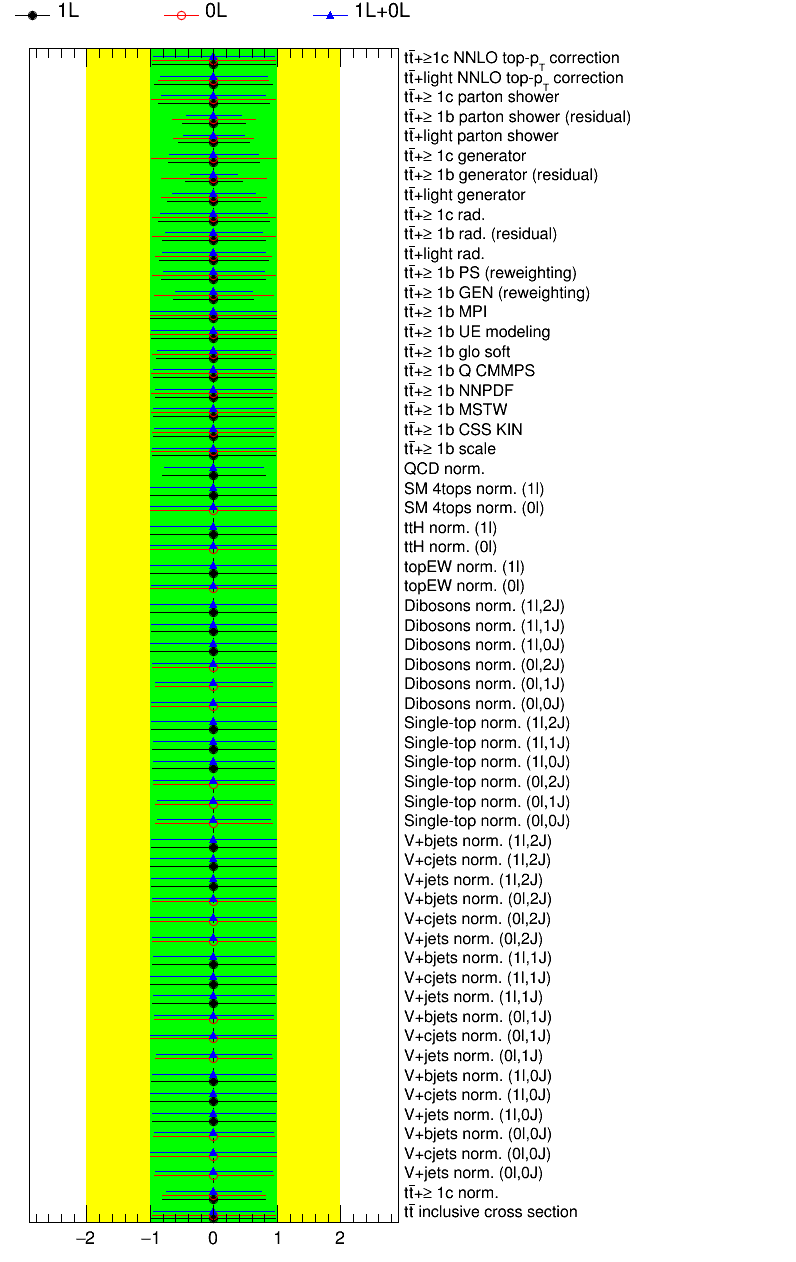
\includegraphics[width=0.9\textwidth]{figures/VLQ/NuisPar_comp_Backgrounduncertainties_Asimov.png}
  \caption*{}
  \label{}
\end{subfigure}
\begin{subfigure}{0.5\textwidth}
  \centering
  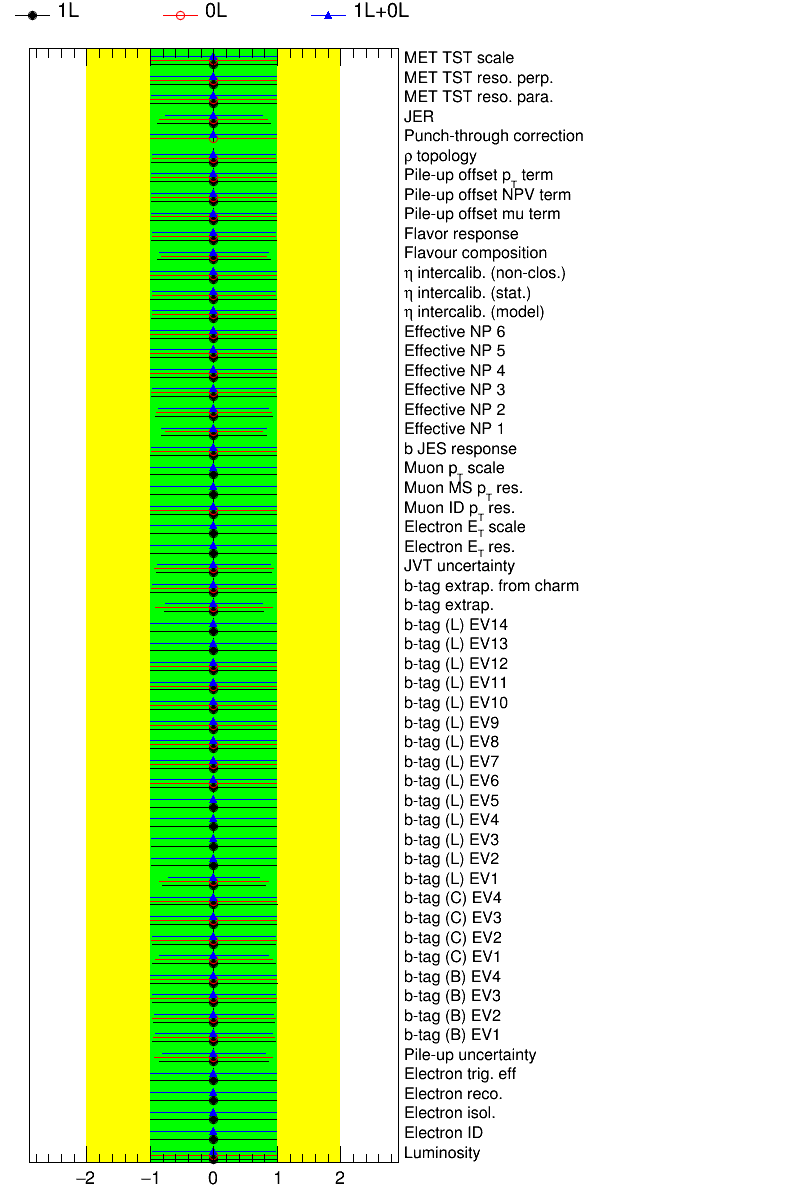
\includegraphics[width=0.9\textwidth]{figures/VLQ/NuisPar_comp_Detectoruncertainties_Asimov.png}
  \caption*{}
  \label{}
\end{subfigure}
\captionsetup{width=0.85\textwidth} \caption{\small Fitted NPs from a fit to the Asimov dataset under the background-only hypothesis. Shown are the fits using the 1-lepton channel only (black), 0-lepton channel only (red), and the combination of both channels (blue). A detailed description of the naming of the NPs can be found in appendix \ref{App:Glossary}.}
\label{sec:vlq:fig:asimovfit}
\end{figure}

For what concerns the detector-related systematic uncertainties, no major constraints are observed with the exception of the pileup uncertainty, jet energy resolution, two components of the jet energy scale uncertainty, the largest component of the $c$-jet and light-jet tagging efficiency uncertainties, and the uncertainty on extrapolation of tagging SFs above the kinematics reach of data used for calibration. The first four uncertainties give a larger contribution at low jet $\pt$ (and hence low $m_{\rm eff}$ ) where large data statistics is available, especially in the 2 and 3 $b$-tagged jets and 0 mass-tagged jets regions. For the largest component of the $c$-jet and light-jet tagging efficiency uncertainties, these are large uncertainties affecting $\ttbar$+light-jets with $\ge4$ $b$-tagged jets, where two of the $b$-tagged jets originate from charm and light-jet mistags.
In the regions with one mass-tagged jet, which requires the presence of energetic objects, there is enough statistics to improve as well the extrapolation at high $\pt$.\par
The analysis is specifically designed to improve background-related systematic uncertainties, particularly those that are potentially overestimated through the comparison of extreme theoretical models, rather than being based on previous data measurements. The fit constraints mostly $t\bar{t}$-related uncertainties since the analysis is dominated by this background. A notable example is the determination of the $t\bar{t}+\ge1b$ normalisation factor, which is determined by the fit, with a precision of about $20\%$. This is due to the large amount of data collected at 13 $\tev$ combined with the event categorisation in multiple jet, $b$-tagged jet and mass-tagged jets multiplicity regions.
After the fit, the uncertainty on the $t\bar{t}+\ge1c$ normalisation is reduced from the initial $50\%$ down to $40\%$, showing the limited sensitivity of this analysis to this background process, mostly coming from the interplay of  regions with 2 and 3 $b$-tagged jets and 0 mass-tagged jets.
The other important aspect is related to the modelling of $t\bar{t}$+light-jets events; the nuisance parameters that are constrained are the ones that correspond to large variations not compatible with the available data precision. This is the case for the radiation, generator and parton-shower uncertainties, which produce effects of up to $30\%$ as a function of the number of jets, while the statistical uncertainty of data in the 3 $b$-tagged jets regions is of the order of few percent.

\subsection{Fit results}
\label{sec:fit:vlqdatafit}
A fit to the data in the 20 analysis regions is performed under the background-only hypothesis, and the fitted NPs are shown in figure \ref{sec:vlq:fig:datafit}. The corresponding correlation matrix for the fitted NPs can be found in figure \ref{sec:vlq:fig:corrmatrix}.

\begin{figure}[htb!]
\begin{subfigure}{0.5\textwidth}
  \centering
  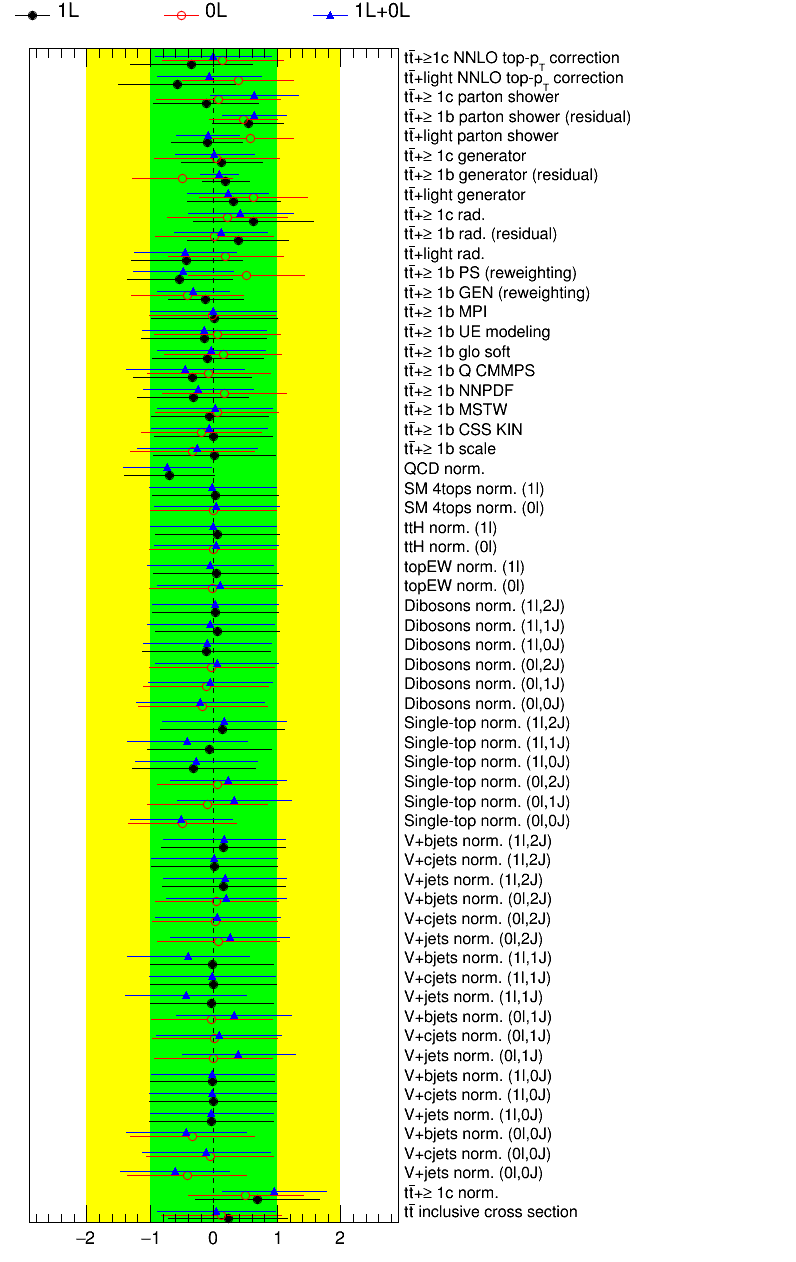
\includegraphics[width=0.9\textwidth]{figures/VLQ/NuisPar_comp_Backgrounduncertainties_Data.png}
  \caption*{}
  \label{}
\end{subfigure}
\begin{subfigure}{0.5\textwidth}
  \centering
  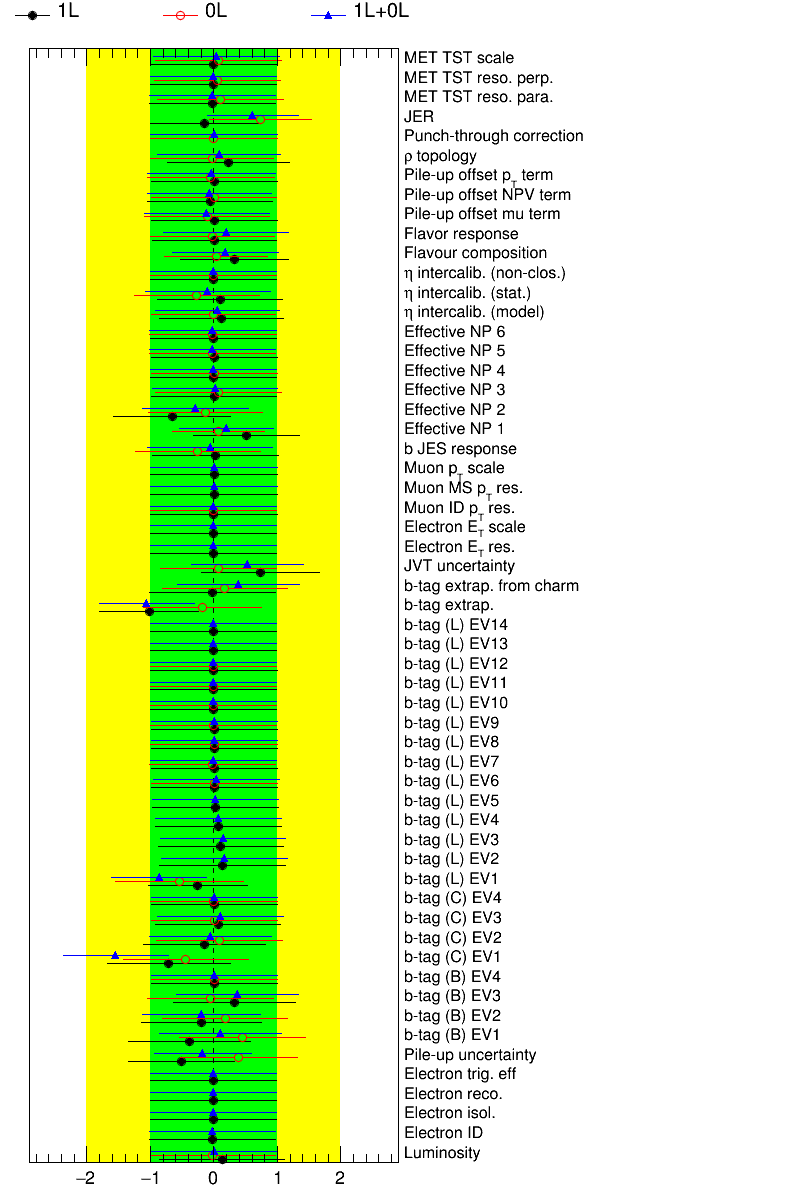
\includegraphics[width=0.9\textwidth]{figures/VLQ/NuisPar_comp_Detectoruncertainties_Data.png}
  \caption*{}
  \label{}
\end{subfigure}
\captionsetup{width=0.85\textwidth} \caption{\small Fitted NPs from a fit under the background-only hypothesis.   Shown are the fits using the 1-lepton channel only (black), 0-lepton channel only (red), and the combination of both channels (blue). A detailed description of the naming of the NPs can be found in appendix \ref{App:Glossary}.}
\label{sec:vlq:fig:datafit}
\end{figure}

\begin{figure}[htb!]
\centering
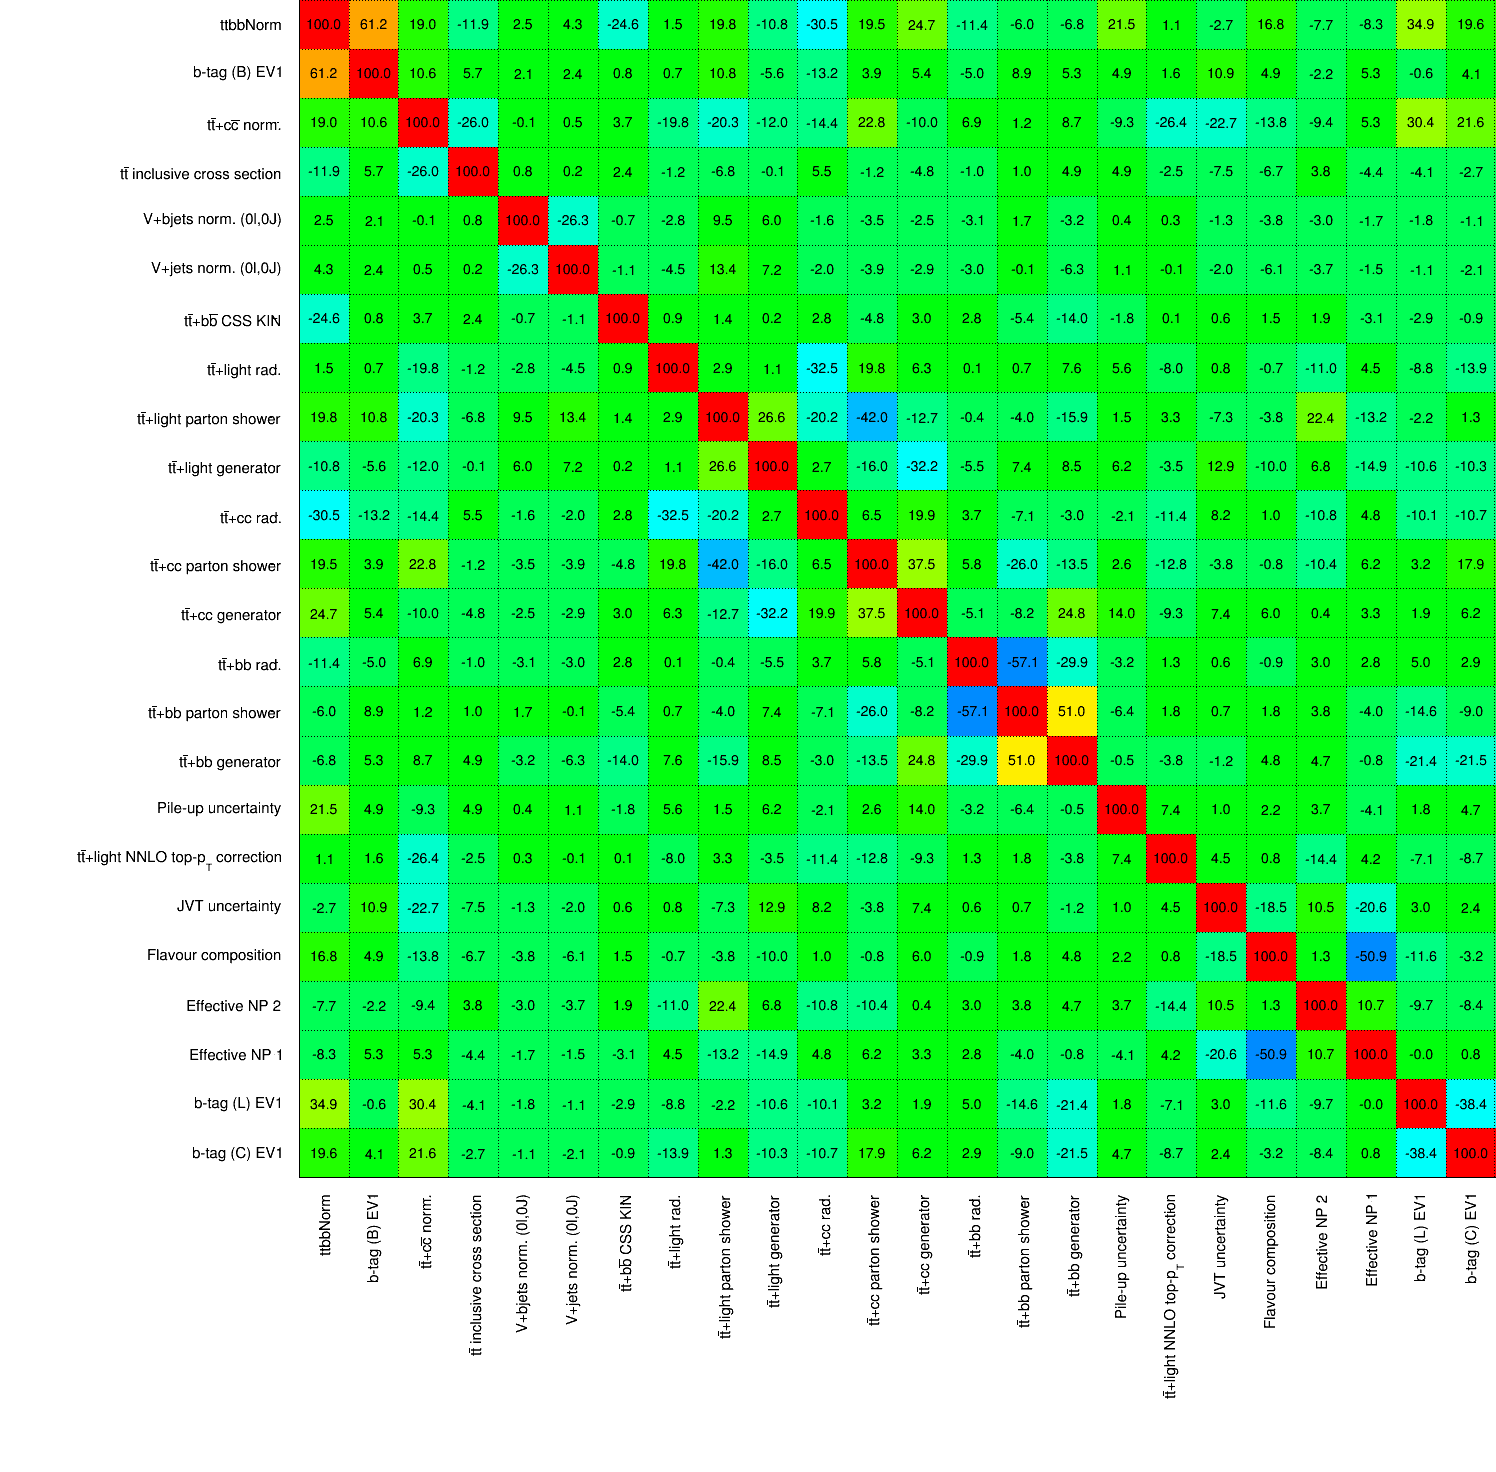
\includegraphics[width=0.5\textwidth]{figures/VLQ/CorrMatrix.png}
\captionsetup{width=0.85\textwidth} \caption{\small Correlation matrix between NPs corresponding to the fit to data under the background-only hypothesis. Only NPs with a correlation coefficient of at least $20\%$ with any other parameter are displayed.}
\label{sec:vlq:fig:corrmatrix}
\end{figure}


Figure \ref{sec:vlq:fig:postfityields} shows the distribution of observed and expected yields in the search regions in the 1-lepton and 0-lepton channels after the combined fit.
\begin{figure}[htb!]
\centering
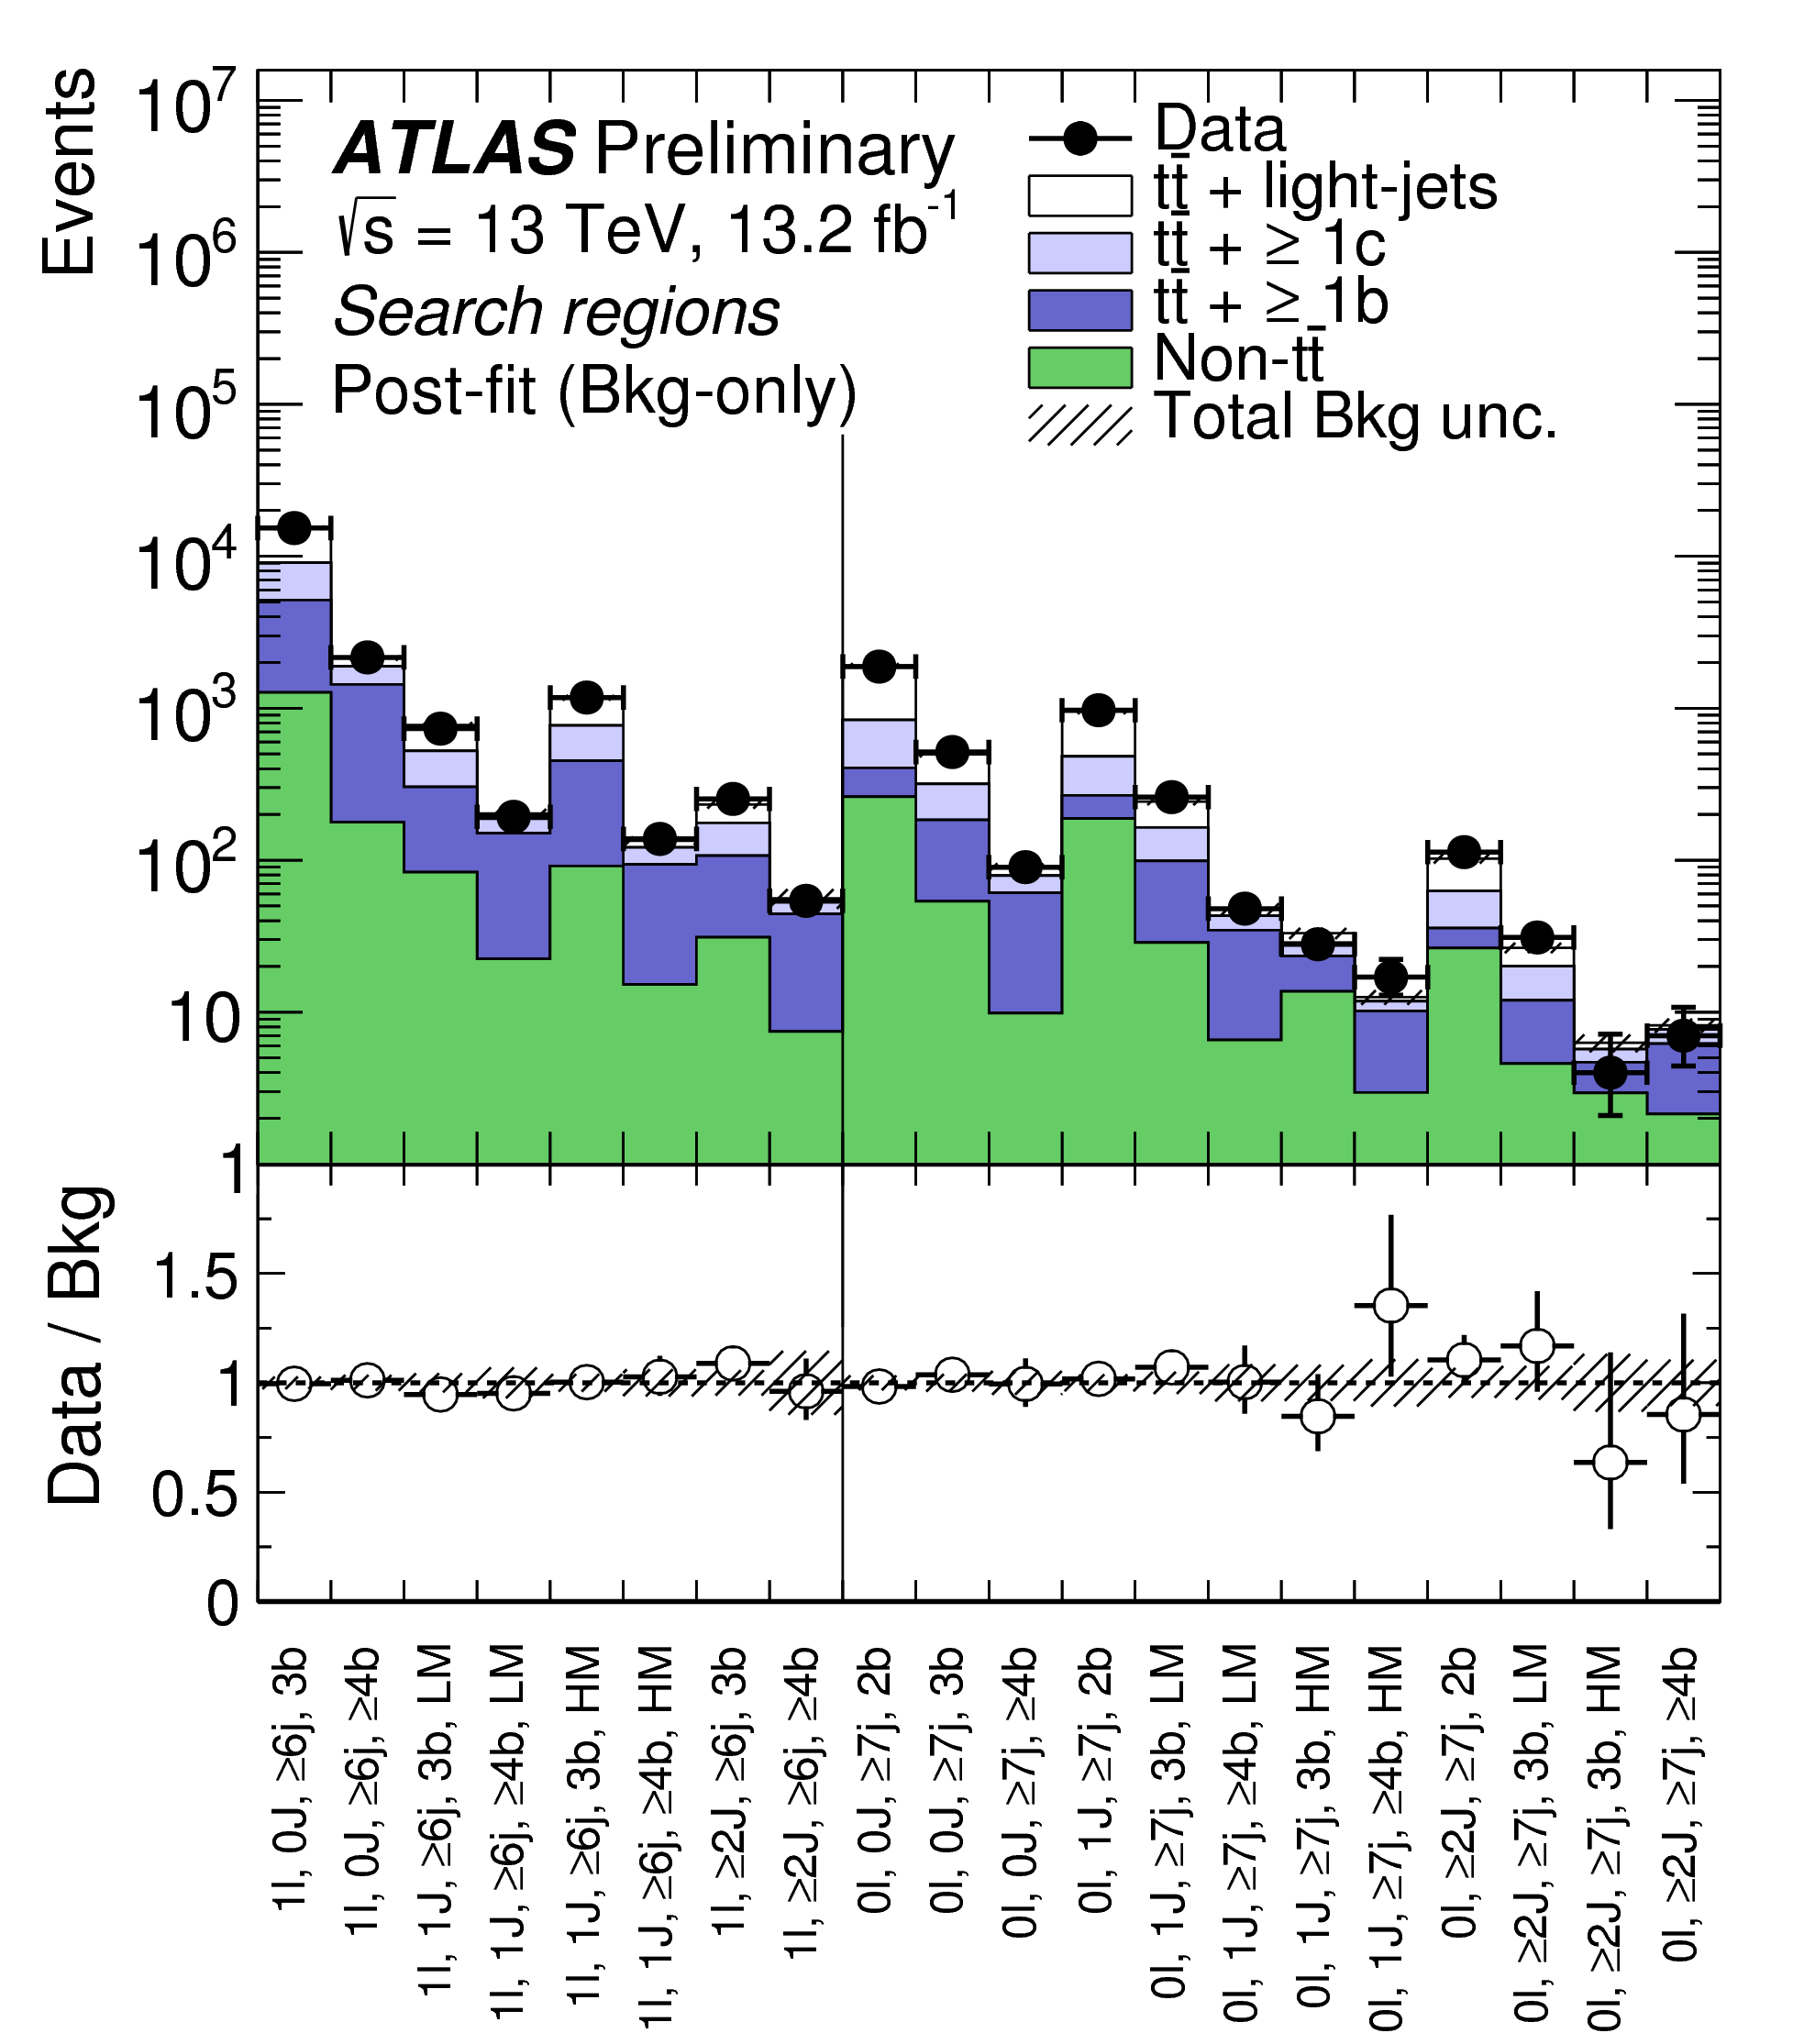
\includegraphics[width=0.5\textwidth]{figures/VLQ/fig_09.png}
\captionsetup{width=0.85\textwidth} \caption{\small Comparison between the data and the background prediction for the yields in the search regions considered in the 1-lepton and 0-lepton channels, after the combined fit to data (``Post-fit") under the background-only hypothesis. The small contributions from $t\bar{t}V$, $t\bar{t} H$, single top, $W/Z$+jets, diboson, and multijet backgrounds are combined into a single background source referred to as ``Non-$t\bar{t}$''. The bottom panel displays the ratio of data to the SM background (``Bkg'') prediction. The hashed area represents the total uncertainty on the background. }
\label{sec:vlq:fig:postfityields}
\end{figure}
The post-fit yields in four of the most sensitive search regions in the 1-lepton and 0-lepton channels can be found in tables \ref{chp:vlq:tab:Postfit_Yields_1L_unblind_COMB} and \ref{chp:vlq:tab:Postfit_Yields_0L_unblind_COMB} respectively.

\begin{table}[htb!]
\begin{center}
\begin{tabular}{l*{4}{c}}
\toprule\toprule
1-lepton channel & 0J, $\geq$6j, $\geq$4b & 1J, $\geq$6j, $\geq$4b & 1J, $\geq$6j, $\geq$4b & $\geq$2J, $\geq$6j, $\geq$4b  \\
& & LM & HM & \\
\midrule\midrule
$t\bar{t}$+light-jets & $ 250 \pm 100 $ &   $ 15.7 \pm 6.6 $ &   $ 13.0 \pm 6.2 $ &   $ 3.3 \pm 1.7 $ \\ 
$t\bar{t}$+$\geq$$1c$ & $ 450 \pm 150 $ &   $ 37 \pm 12 $ &   $ 28 \pm 10 $ &   $ 8.5 \pm 3.3 $ \\ 
$t\bar{t}$+$\geq$$1b$ & $ 1260 \pm 130$ &   $ 128 \pm 17 $ &   $ 79 \pm 10 $ &   $ 36.9 \pm 7.7 $ \\  
$t\bar{t}V$ & $ 30 \pm 10 $ &   $ 4.7 \pm 1.5 $ &   $ 2.54 \pm 0.85 $ &   $ 1.33 \pm 0.44 $ \\   
$t\bar{t}H$ & $ 57 \pm 18 $ &   $ 6.3 \pm 2.1 $ &   $ 5.9 \pm 2.0 $ &   $ 2.28 \pm 0.76 $ \\ 
$W$+jets & $ 26 \pm 11 $ &   $ 3.6 \pm 1.6 $ &   $ 1.05 \pm 0.45 $ &   $ 0.85 \pm 0.41 $ \\ 
$Z$+jets & $ 5.3 \pm 2.3 $ &   $ 0.49 \pm 0.37 $ &   $ 0.12 \pm 0.06 $ &   $ 0.16 \pm 0.09 $ \\ 
Single top & $ 52 \pm 14 $ &   $ 5.4 \pm 1.5 $ &   $ 4.4 \pm 1.3 $ &   $ 1.61 \pm 0.70 $ \\ 
Diboson & $ 4.6 \pm 2.4 $ &   $ 0.76 \pm 0.51 $ &   $ 0.09 \pm 0.20 $ &   $ 0.10 \pm 0.06 $ \\ 
$t\bar{t}t\bar{t}$ (SM) & $ 3.2 \pm 1.0 $ &   $ 1.17 \pm 0.38 $ &   $ 1.09 \pm 0.36 $ &   $ 1.11 \pm 0.36 $ \\ 
%Multijet & -- &  --  &  --  &  --  \\ 
\midrule
Total background & $ 2135 \pm 79 $ &   $ 203 \pm 15 $ &   $ 134.3 \pm 8.7 $ &   $ 56.2 \pm 8.3 $ \\ 
\midrule
Data &  2160  & 193  & 138  & 54  \\ 
\bottomrule\bottomrule     \\
\end{tabular}
%%\\
\vspace{0.1cm}

%
\end{center}
\vspace{-0.5cm}
\captionsetup{width=0.85\textwidth} \caption{\small Predicted and observed yields in the 1-lepton channel in four of the most-sensitive search regions considered. The multijet background is considered negligible in these regions and thus not shown. The background prediction is shown after the combined fit to data in the 0-lepton and 1-lepton channels under the background-only hypothesis. The quoted uncertainties are the sum in quadrature of statistical and systematic uncertainties on the yields, computed taking into account correlations among nuisance parameters and among processes. }
\label{chp:vlq:tab:Postfit_Yields_1L_unblind_COMB}
\end{table}
%%%%%%%%%%%%%%%%%%%%%%%%%%%%%%%%%%%%%%%%%%%%%%%%%% 
%%%%%%%%%%%%%%%%%%%%%%%%%%%%%%%%%%%%%%%%%%%%%%%%%% 
\begin{table}[htb!]
\begin{center}
\begin{tabular}{l*{4}{c}}
\toprule\toprule
0-lepton channel & 1J, $\geq$7j, $\geq$4b & 2J, $\geq$7j, $\geq$2b & $\geq$2J, $\geq$7j, 3b & $\geq$2J, $\geq$7j, $\geq$4b  \\
& HM & & HM & \\
\midrule\midrule
$t\bar{t}$+light-jets & $ 0.76 \pm 0.31 $ &   $ 39.7 \pm 6.7 $ &   $ 0.58 \pm 0.16 $ &   $ 0.50 \pm 0.21 $ \\ 
$t\bar{t}$+$\geq$$1c$ & $ 1.66 \pm 0.55 $ &   $ 27 \pm 10 $ &   $ 1.02 \pm 0.36 $ &   $ 1.47 \pm 0.52 $ \\  
$t\bar{t}$+$\geq$$1b$ & $ 7.2 \pm 1.5 $ &   $ 9.3 \pm 2.8 $ &   $ 1.75 \pm 0.47 $ &   $ 4.08 \pm 0.83 $ \\
$t\bar{t}V$ & $ 0.52 \pm 0.11 $ &   $ 3.86 \pm 0.63 $ &   $ 0.48 \pm 0.09 $ &   $ 0.33 \pm 0.07 $ \\  
$t\bar{t}H$ & $ 0.50 \pm 0.09 $ &   $ 0.71 \pm 0.10 $ &   $ 0.12 \pm 0.02 $ &   $ 0.33 \pm 0.07 $ \\
$W$+jets & $ 0.58 \pm 0.25 $ &   $ 7.0 \pm 2.6 $ &   $ 0.44 \pm 0.18 $ &   $ 0.30 \pm 0.16 $ \\
$Z$+jets & $ 0.56 \pm 0.25 $ &   $ 4.9 \pm 1.9 $ &   $ 0.40 \pm 0.17 $ &   $ 0.10 \pm 0.12 $ \\
Single top & $ 0.55 \pm 0.31 $ &   $ 6.6 \pm 3.4 $ &   $ 0.90 \pm 0.54 $ &   $ 0.36 \pm 0.24 $ \\ 
Diboson & $ 0.13 \pm 0.15 $ &   $ 3.2 \pm 2.0 $ &   $ 0.55 \pm 0.63 $ &   $ 0.49 \pm 0.47 $ \\ 
$t\bar{t}t\bar{t}$ (SM) &  $ 0.11 \pm 0.04 $ &   $ 0.23 \pm 0.08 $ &   $ 0.05 \pm 0.02 $ &   $ 0.22 \pm 0.07 $ \\  
\midrule
Total background & $ 12.6 \pm 1.4 $ &   $ 102.3 \pm 7.0 $ &   $ 6.3 \pm 1.0 $ &   $ 8.2 \pm 1.0 $ \\ 
\midrule
Data &  17  & 113  & 4  & 7  \\ 
\bottomrule\bottomrule     \\
\end{tabular}
%%\\
\vspace{0.1cm}

%
\end{center}
\vspace{-0.5cm}
\captionsetup{width=0.85\textwidth} \caption{\small Predicted and observed yields in the 0-lepton channel in four of the most-sensitive search regions considered. The multijet background is considered negligible in these regions and thus not shown. The background prediction is shown after the combined fit to data in the 0-lepton and 1-lepton channels under the background-only hypothesis. The quoted uncertainties are the sum in quadrature of statistical and systematic uncertainties on the yields, computed taking into account correlations among nuisance parameters and among processes. }
\label{chp:vlq:tab:Postfit_Yields_0L_unblind_COMB}
\end{table}
Figures \ref{sec:vlq:fig:meff1} and \ref{sec:vlq:fig:meff3}  show the comparison of data and prediction for the $m_{\rm eff}$ distributions in the most-sensitive search regions in the 1-lepton and 0-lepton channels respectively, before and after the fit to data. 


\begin{figure}[p!]
\begin{subfigure}{0.24\textwidth}
  \centering
  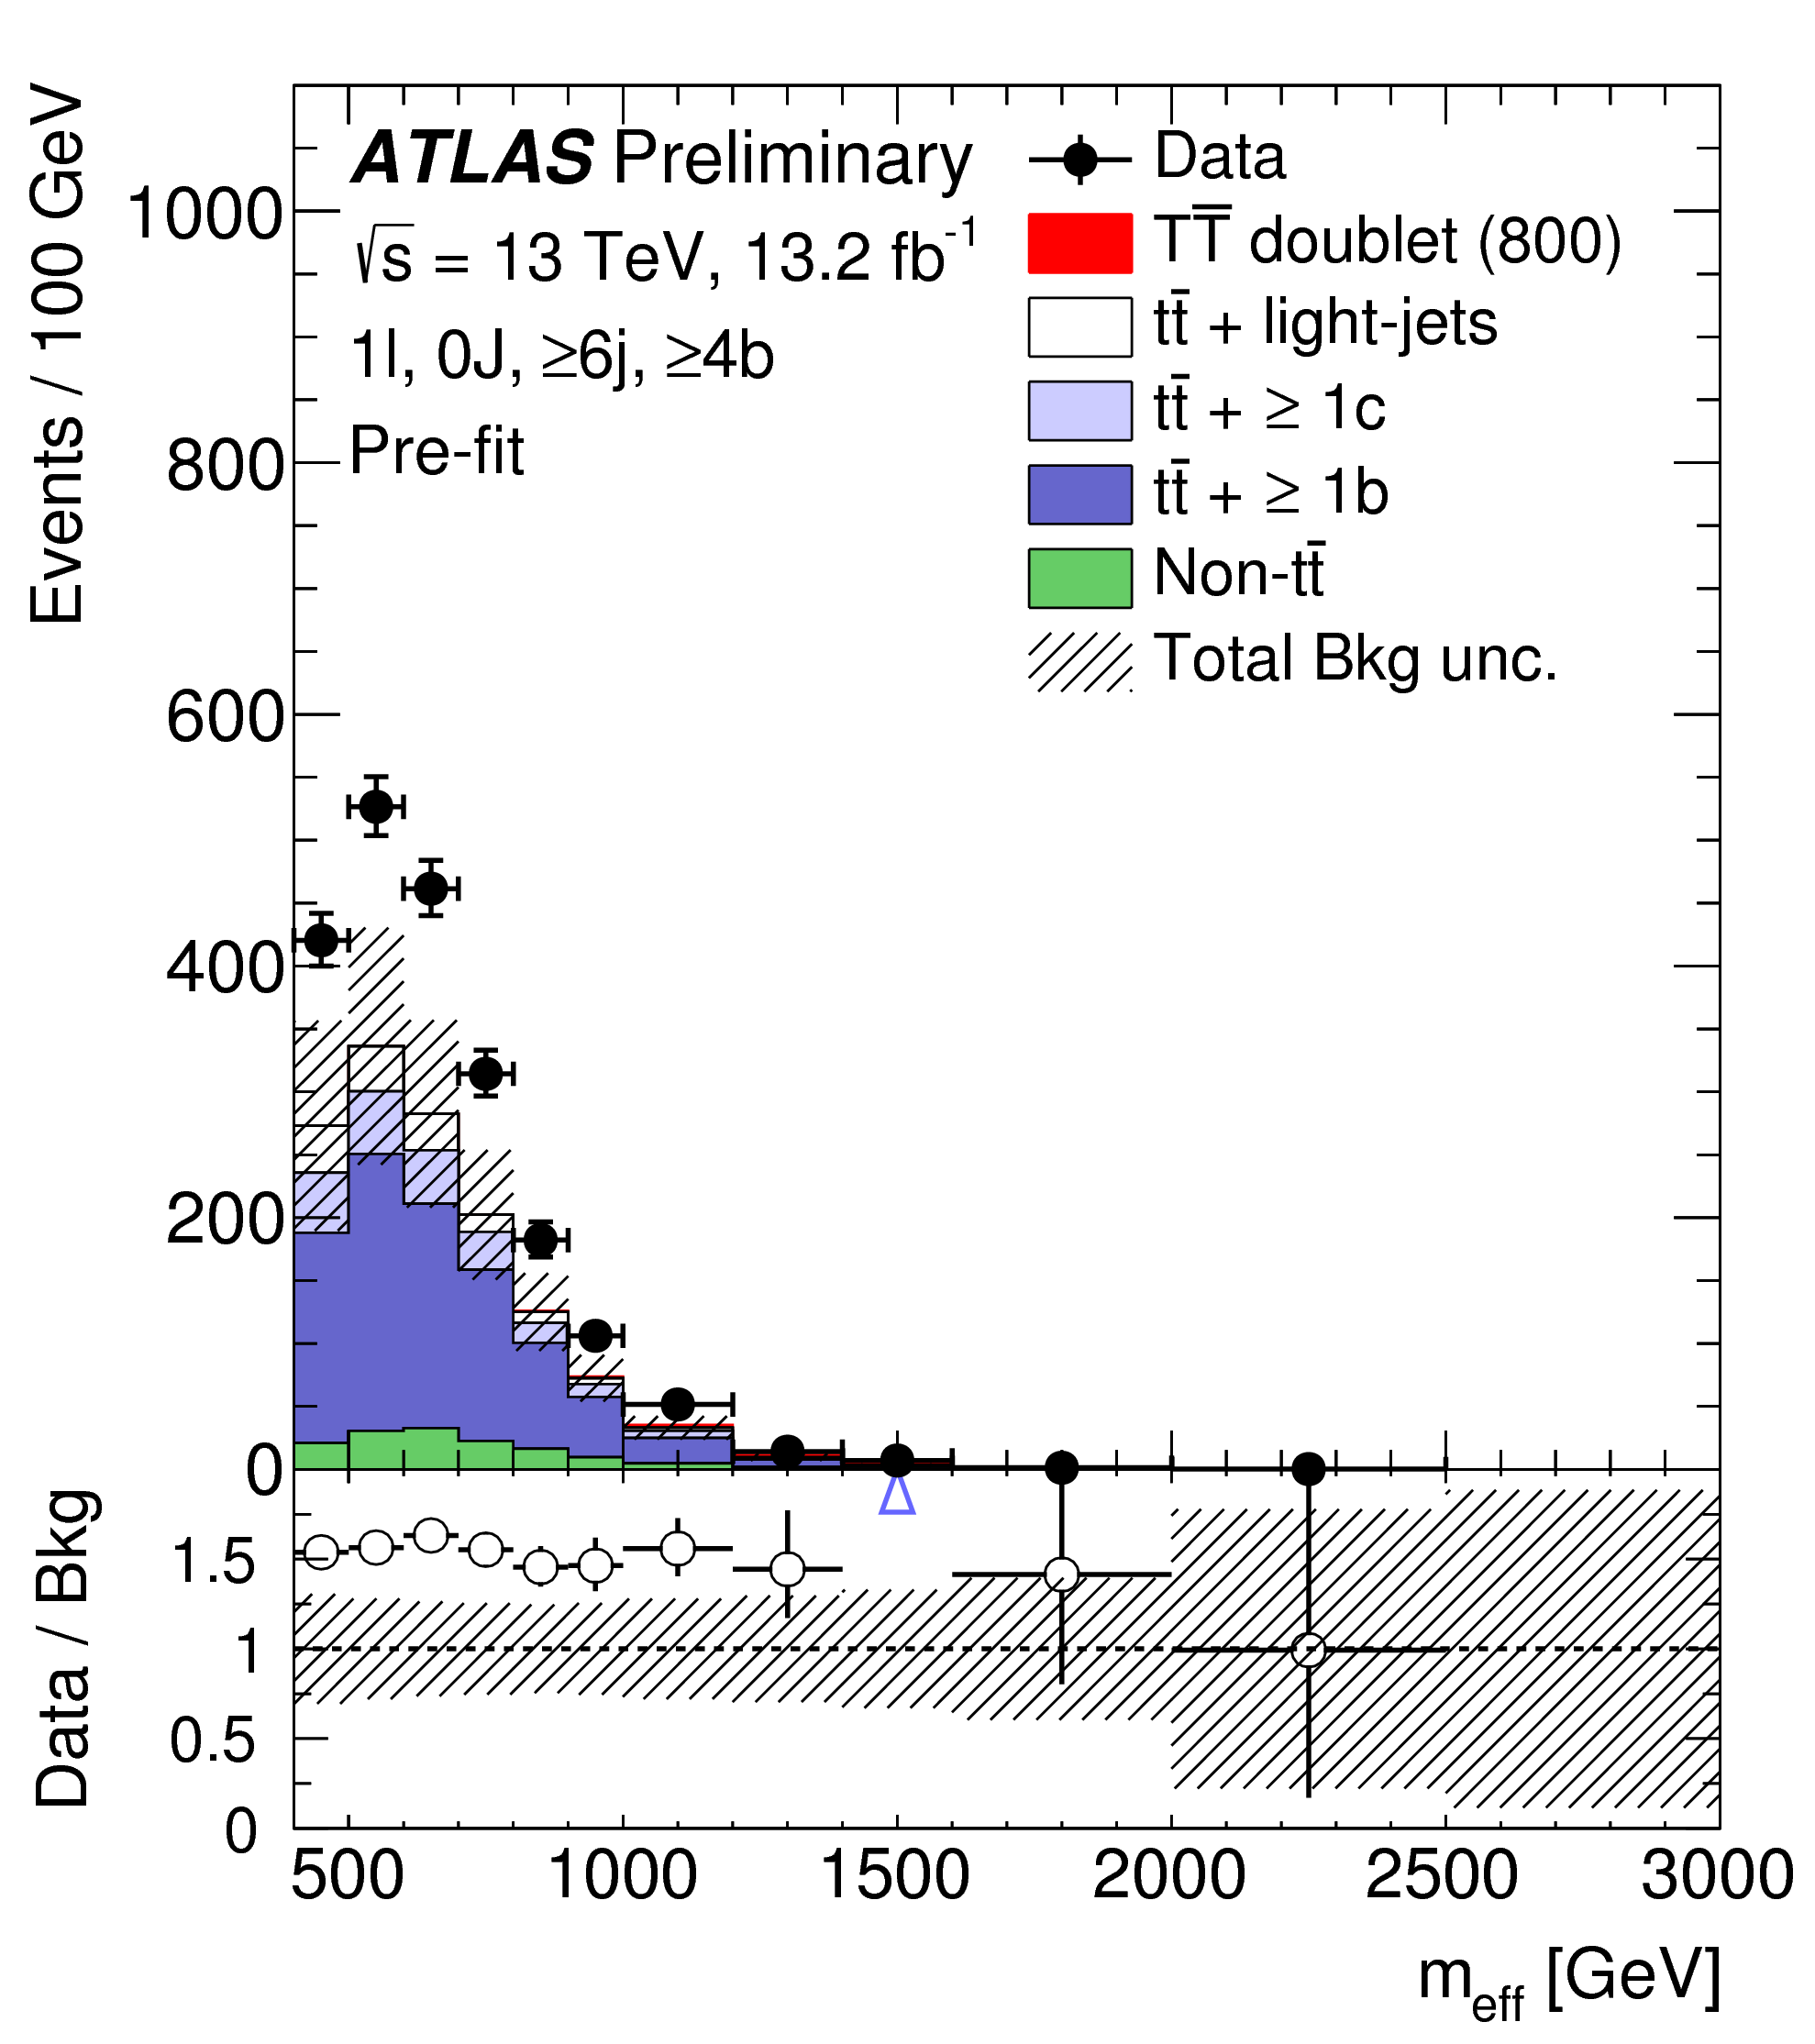
\includegraphics[width=0.9\textwidth]{figures/VLQ/fig_10a.png}
  \caption{}
  \label{}
\end{subfigure}
\begin{subfigure}{0.24\textwidth}
  \centering
  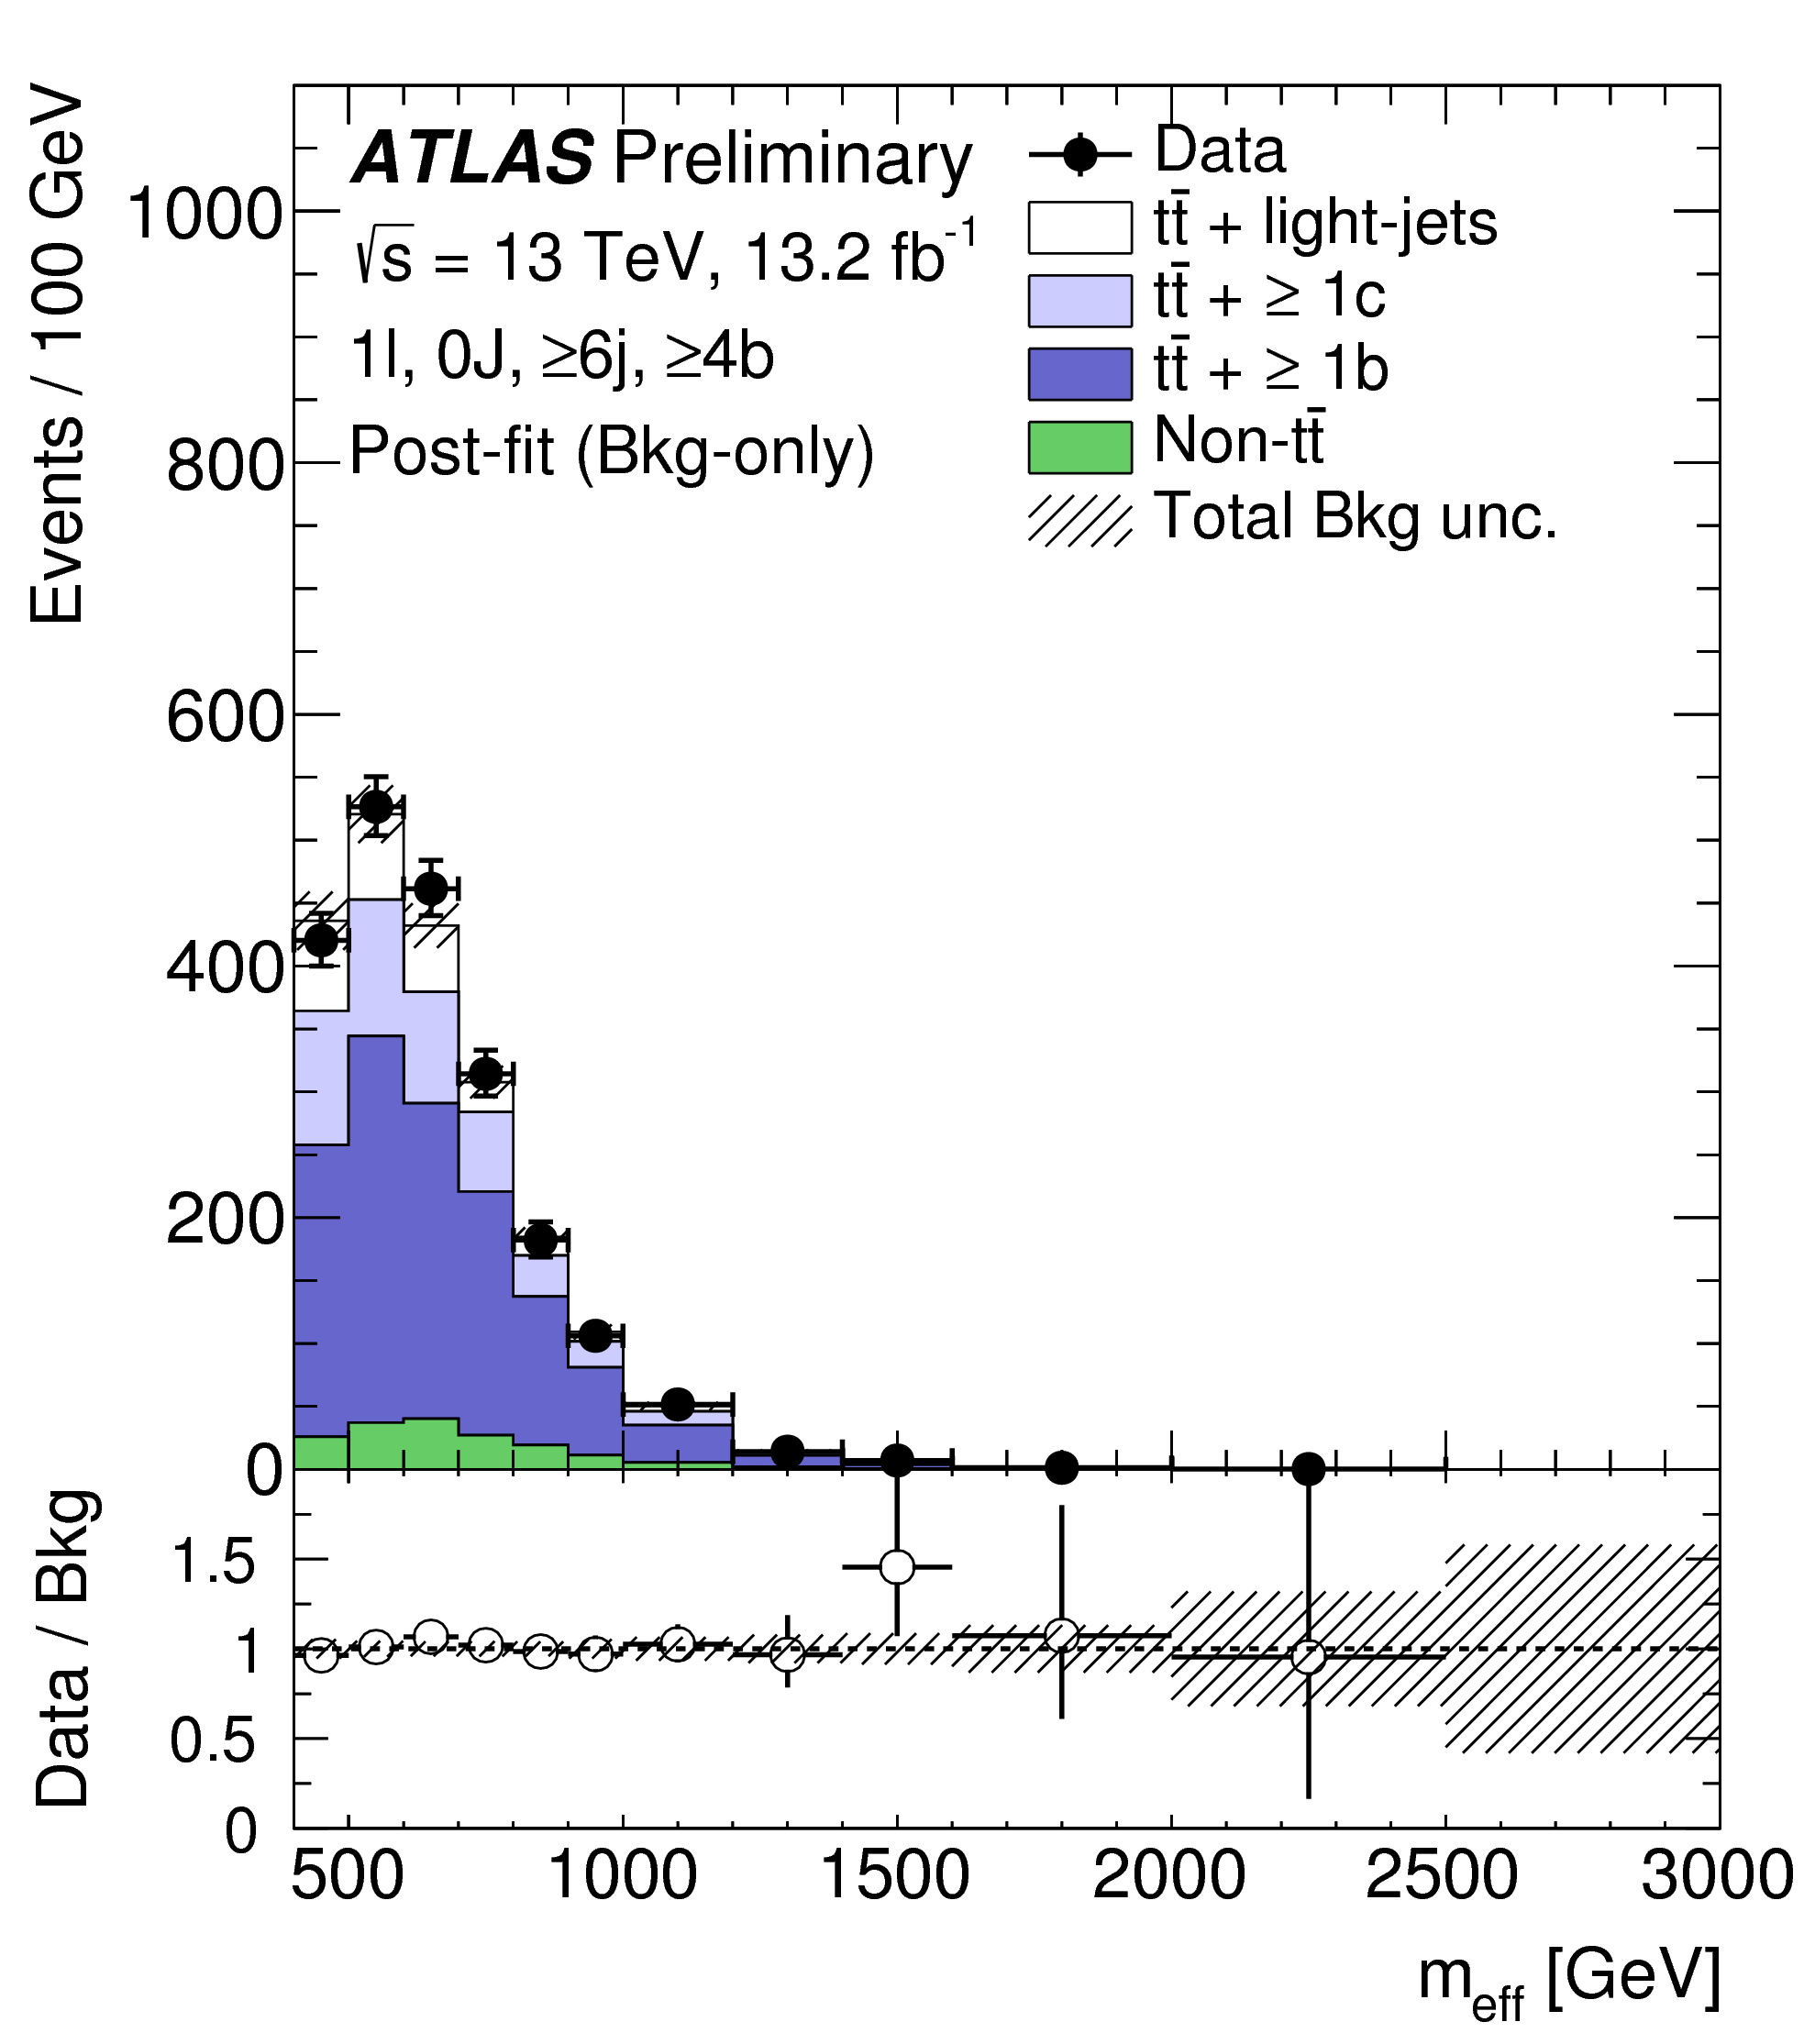
\includegraphics[width=0.9\textwidth]{figures/VLQ/fig_10b.png}
  \caption{}
  \label{}
\end{subfigure}
\begin{subfigure}{0.24\textwidth}
  \centering
  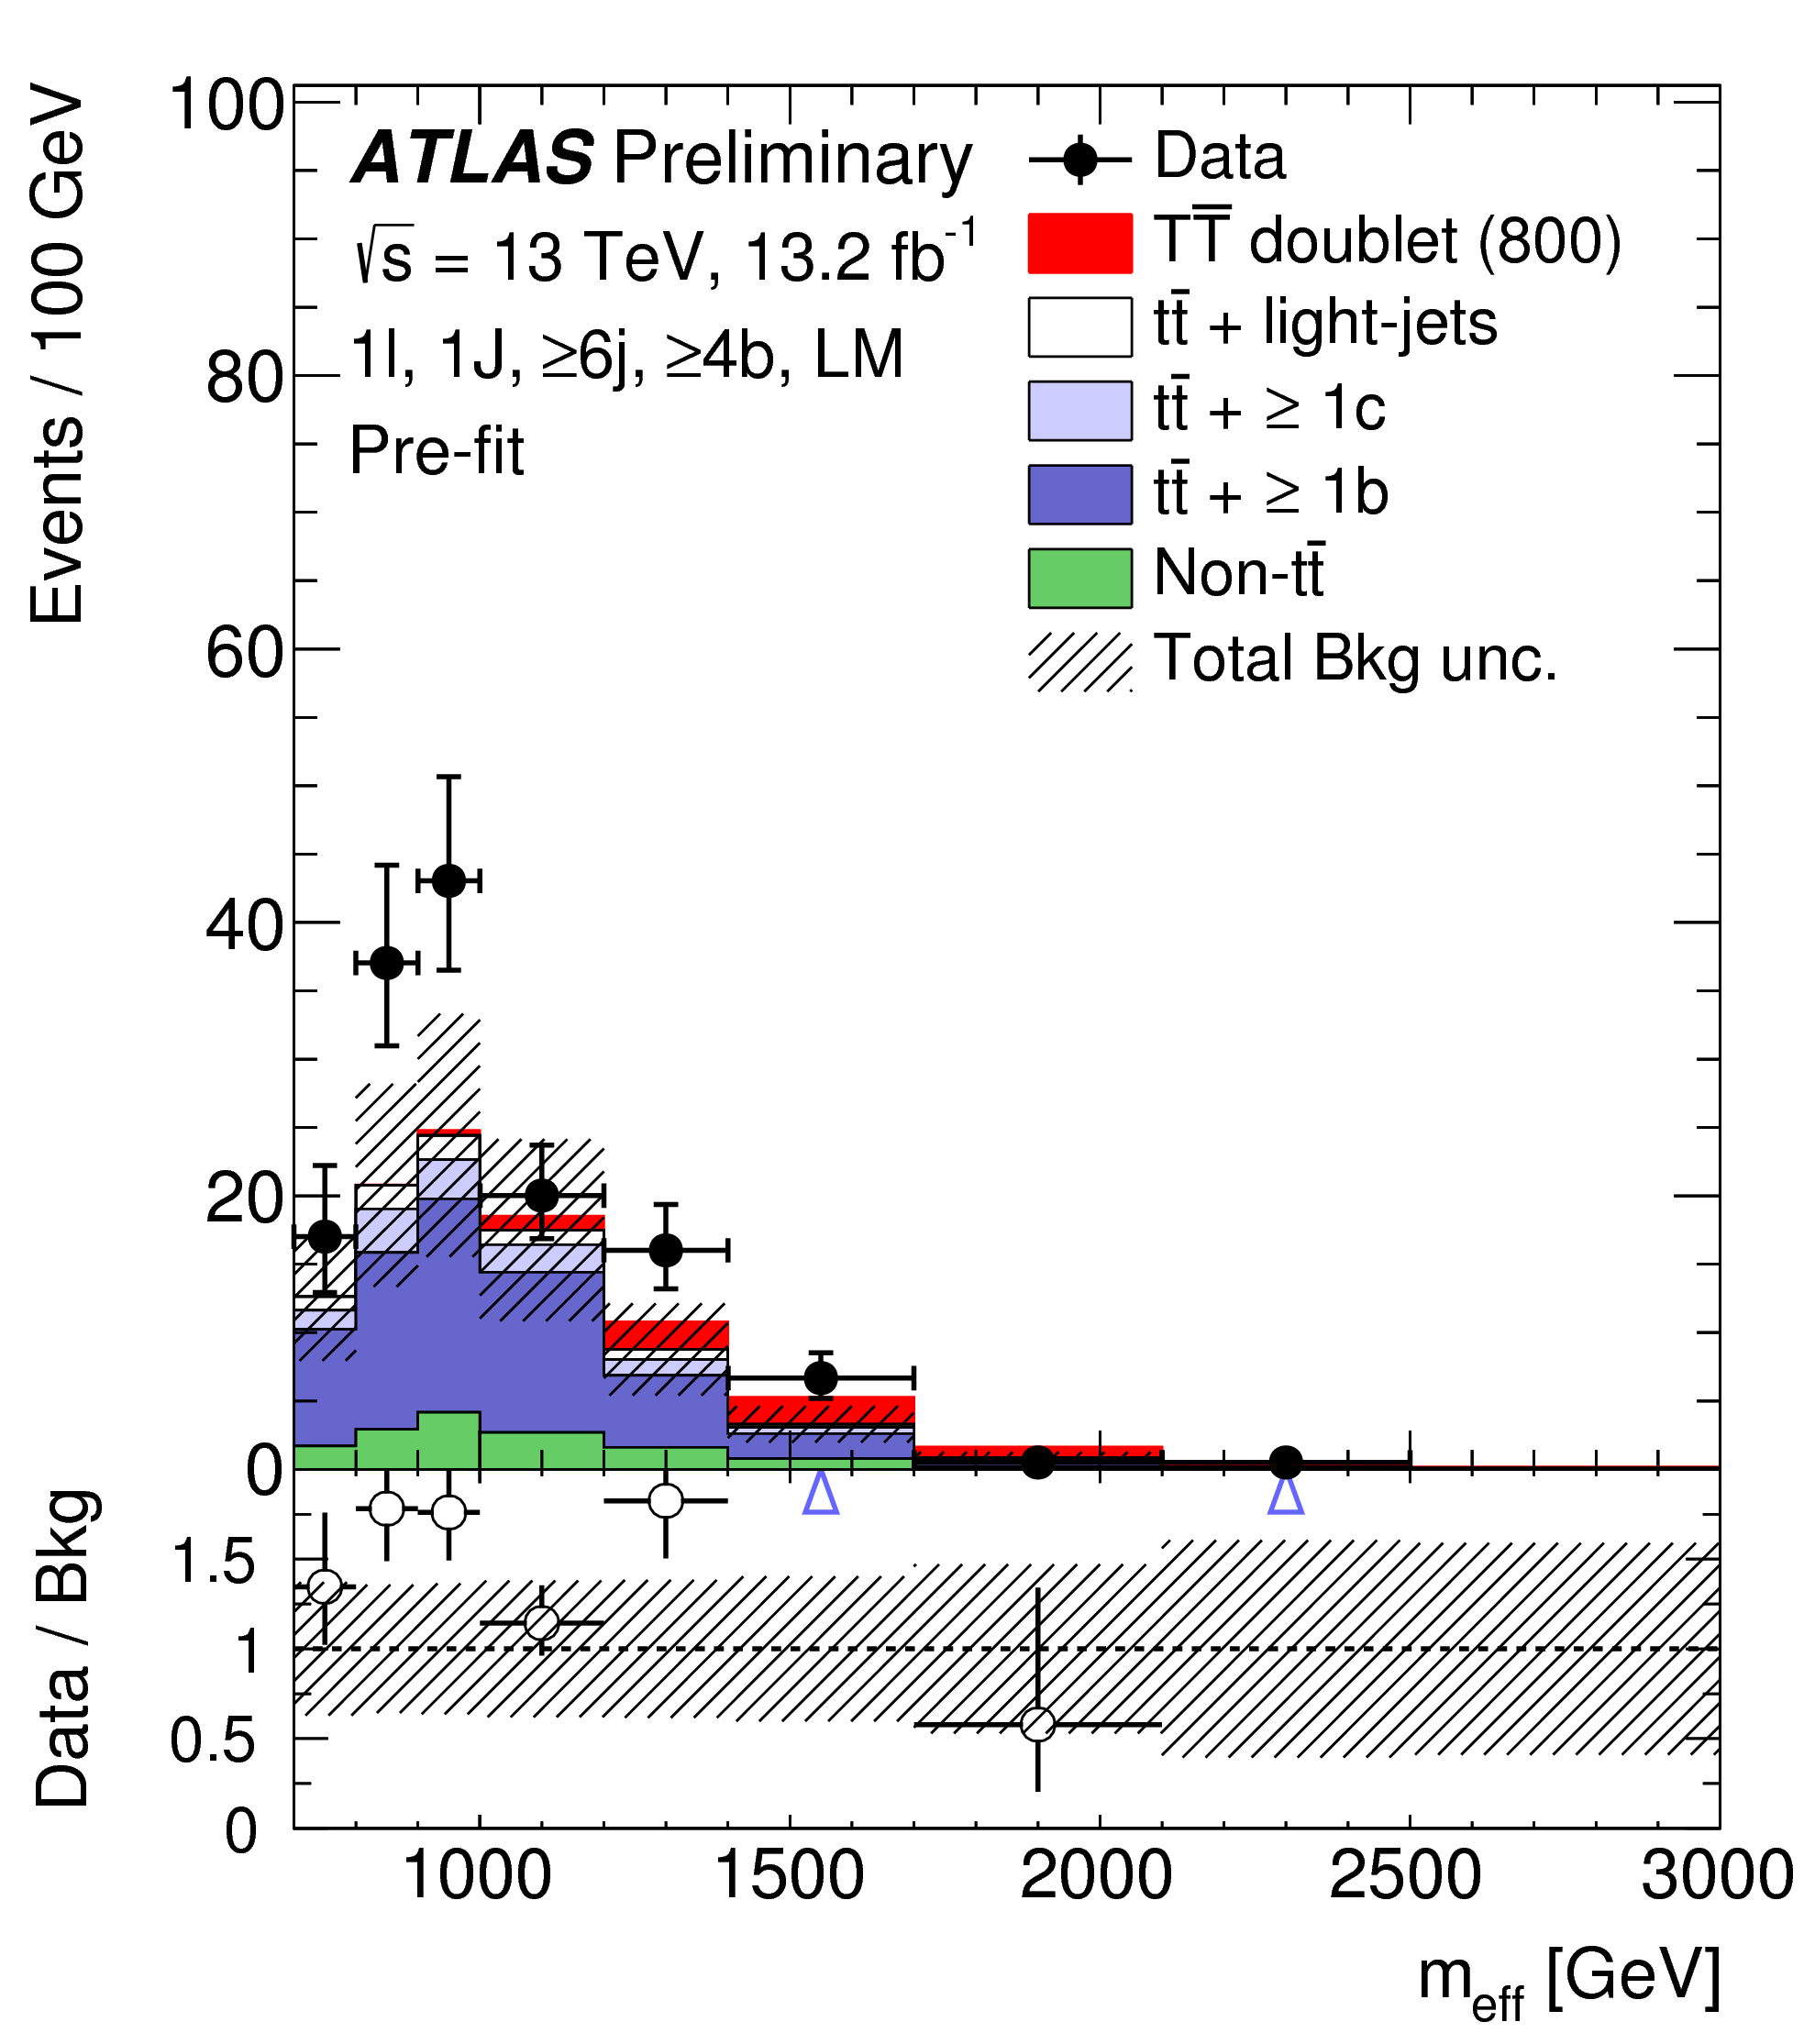
\includegraphics[width=0.9\textwidth]{figures/VLQ/fig_10c.png}
  \caption{}
  \label{}
\end{subfigure}
\begin{subfigure}{0.24\textwidth}
  \centering
  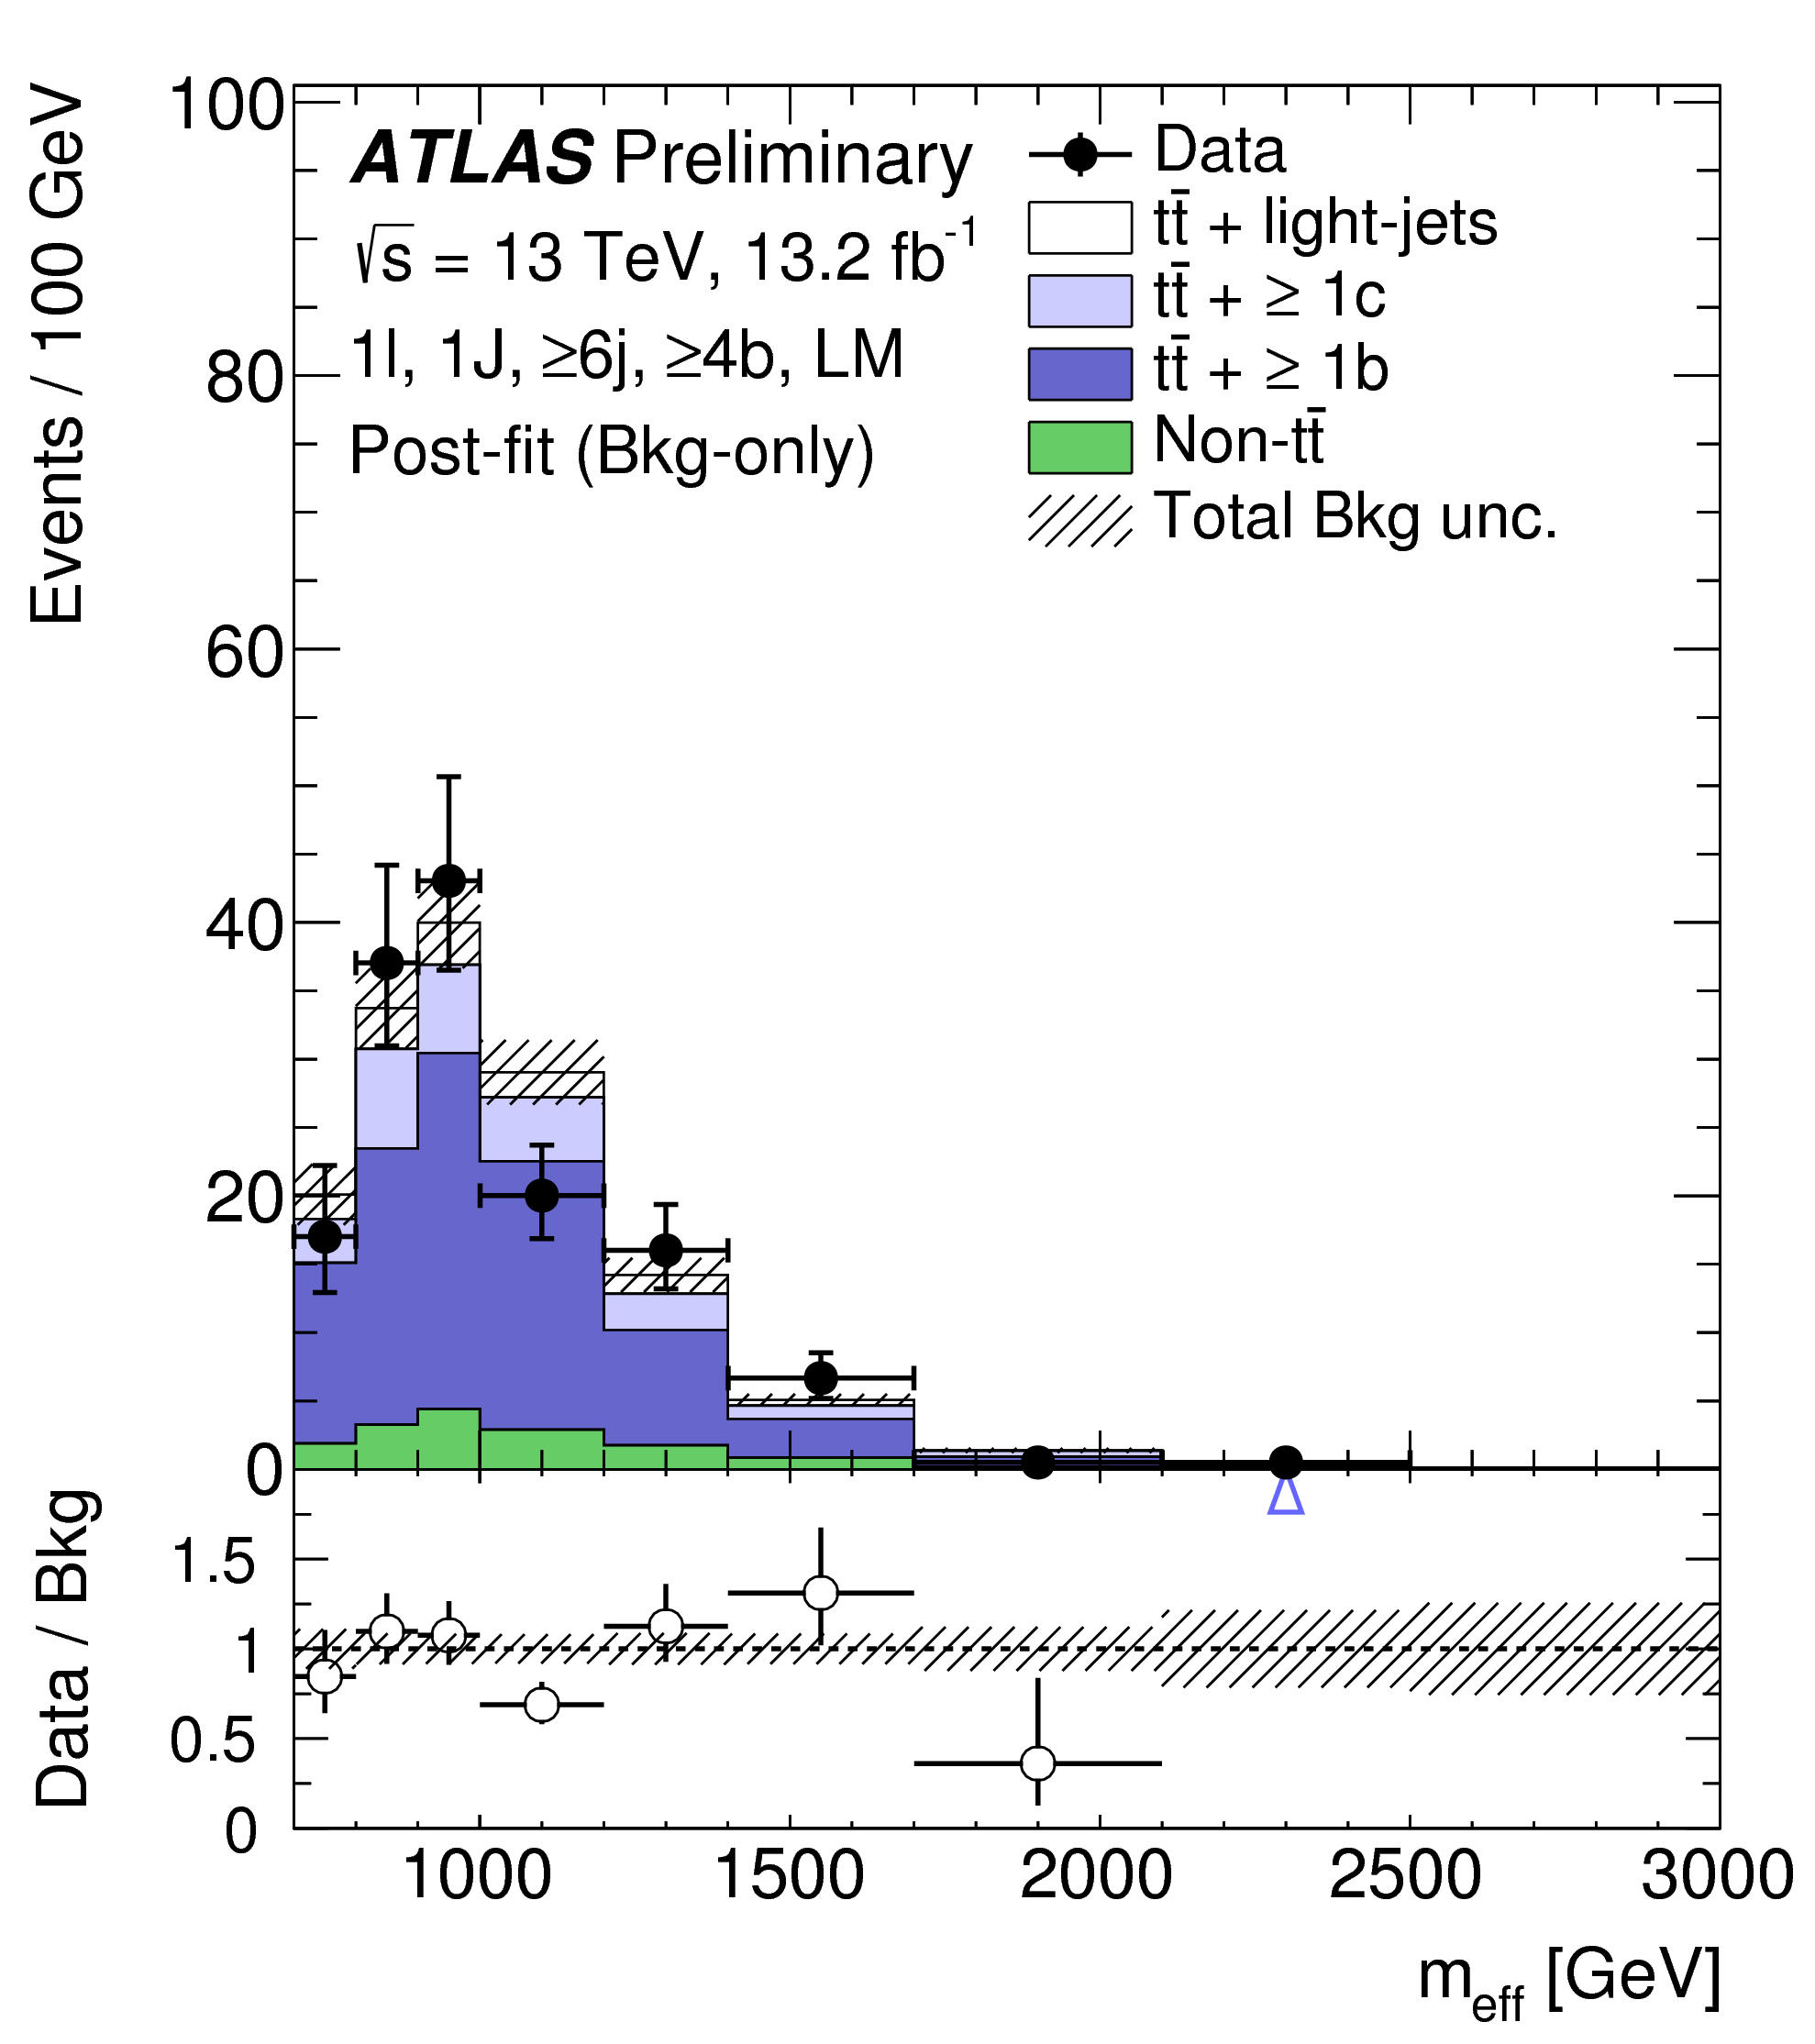
\includegraphics[width=0.9\textwidth]{figures/VLQ/fig_10d.png}
  \caption{}
  \label{}
\end{subfigure}
\begin{subfigure}{0.24\textwidth}
  \centering
  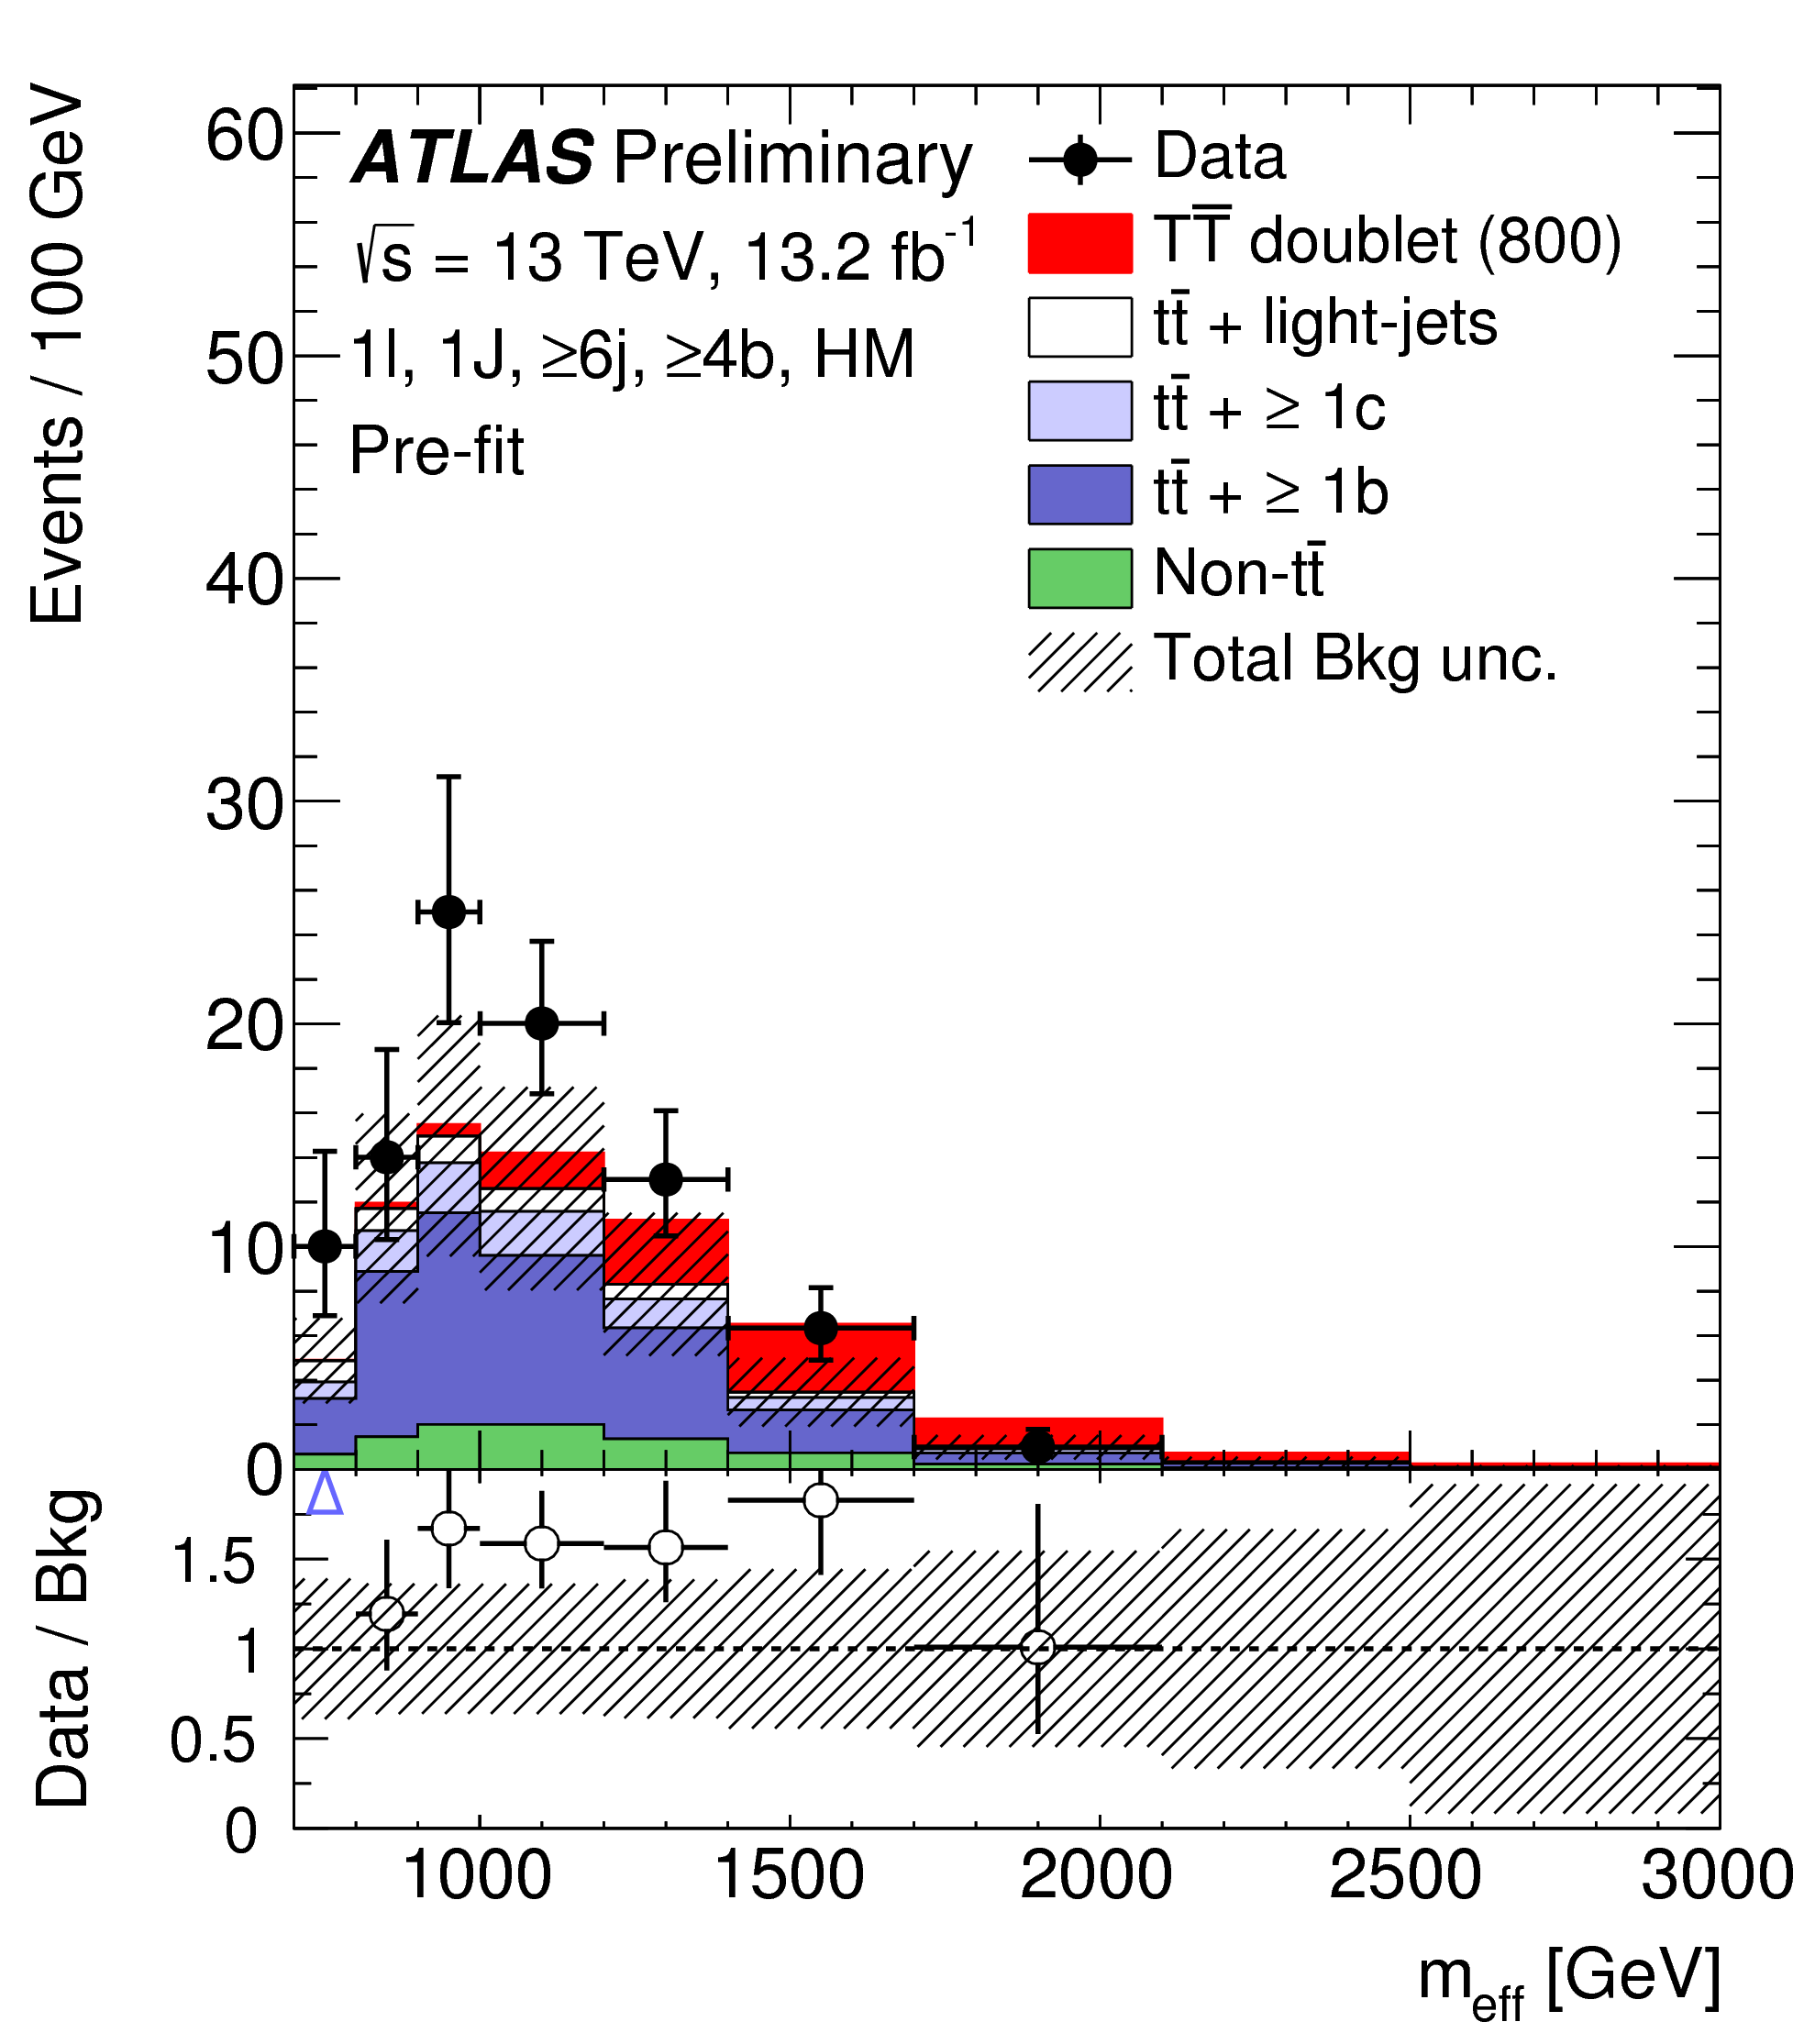
\includegraphics[width=0.9\textwidth]{figures/VLQ/fig_11a.png}
  \caption{}
  \label{}
\end{subfigure}
\begin{subfigure}{0.24\textwidth}
  \centering
  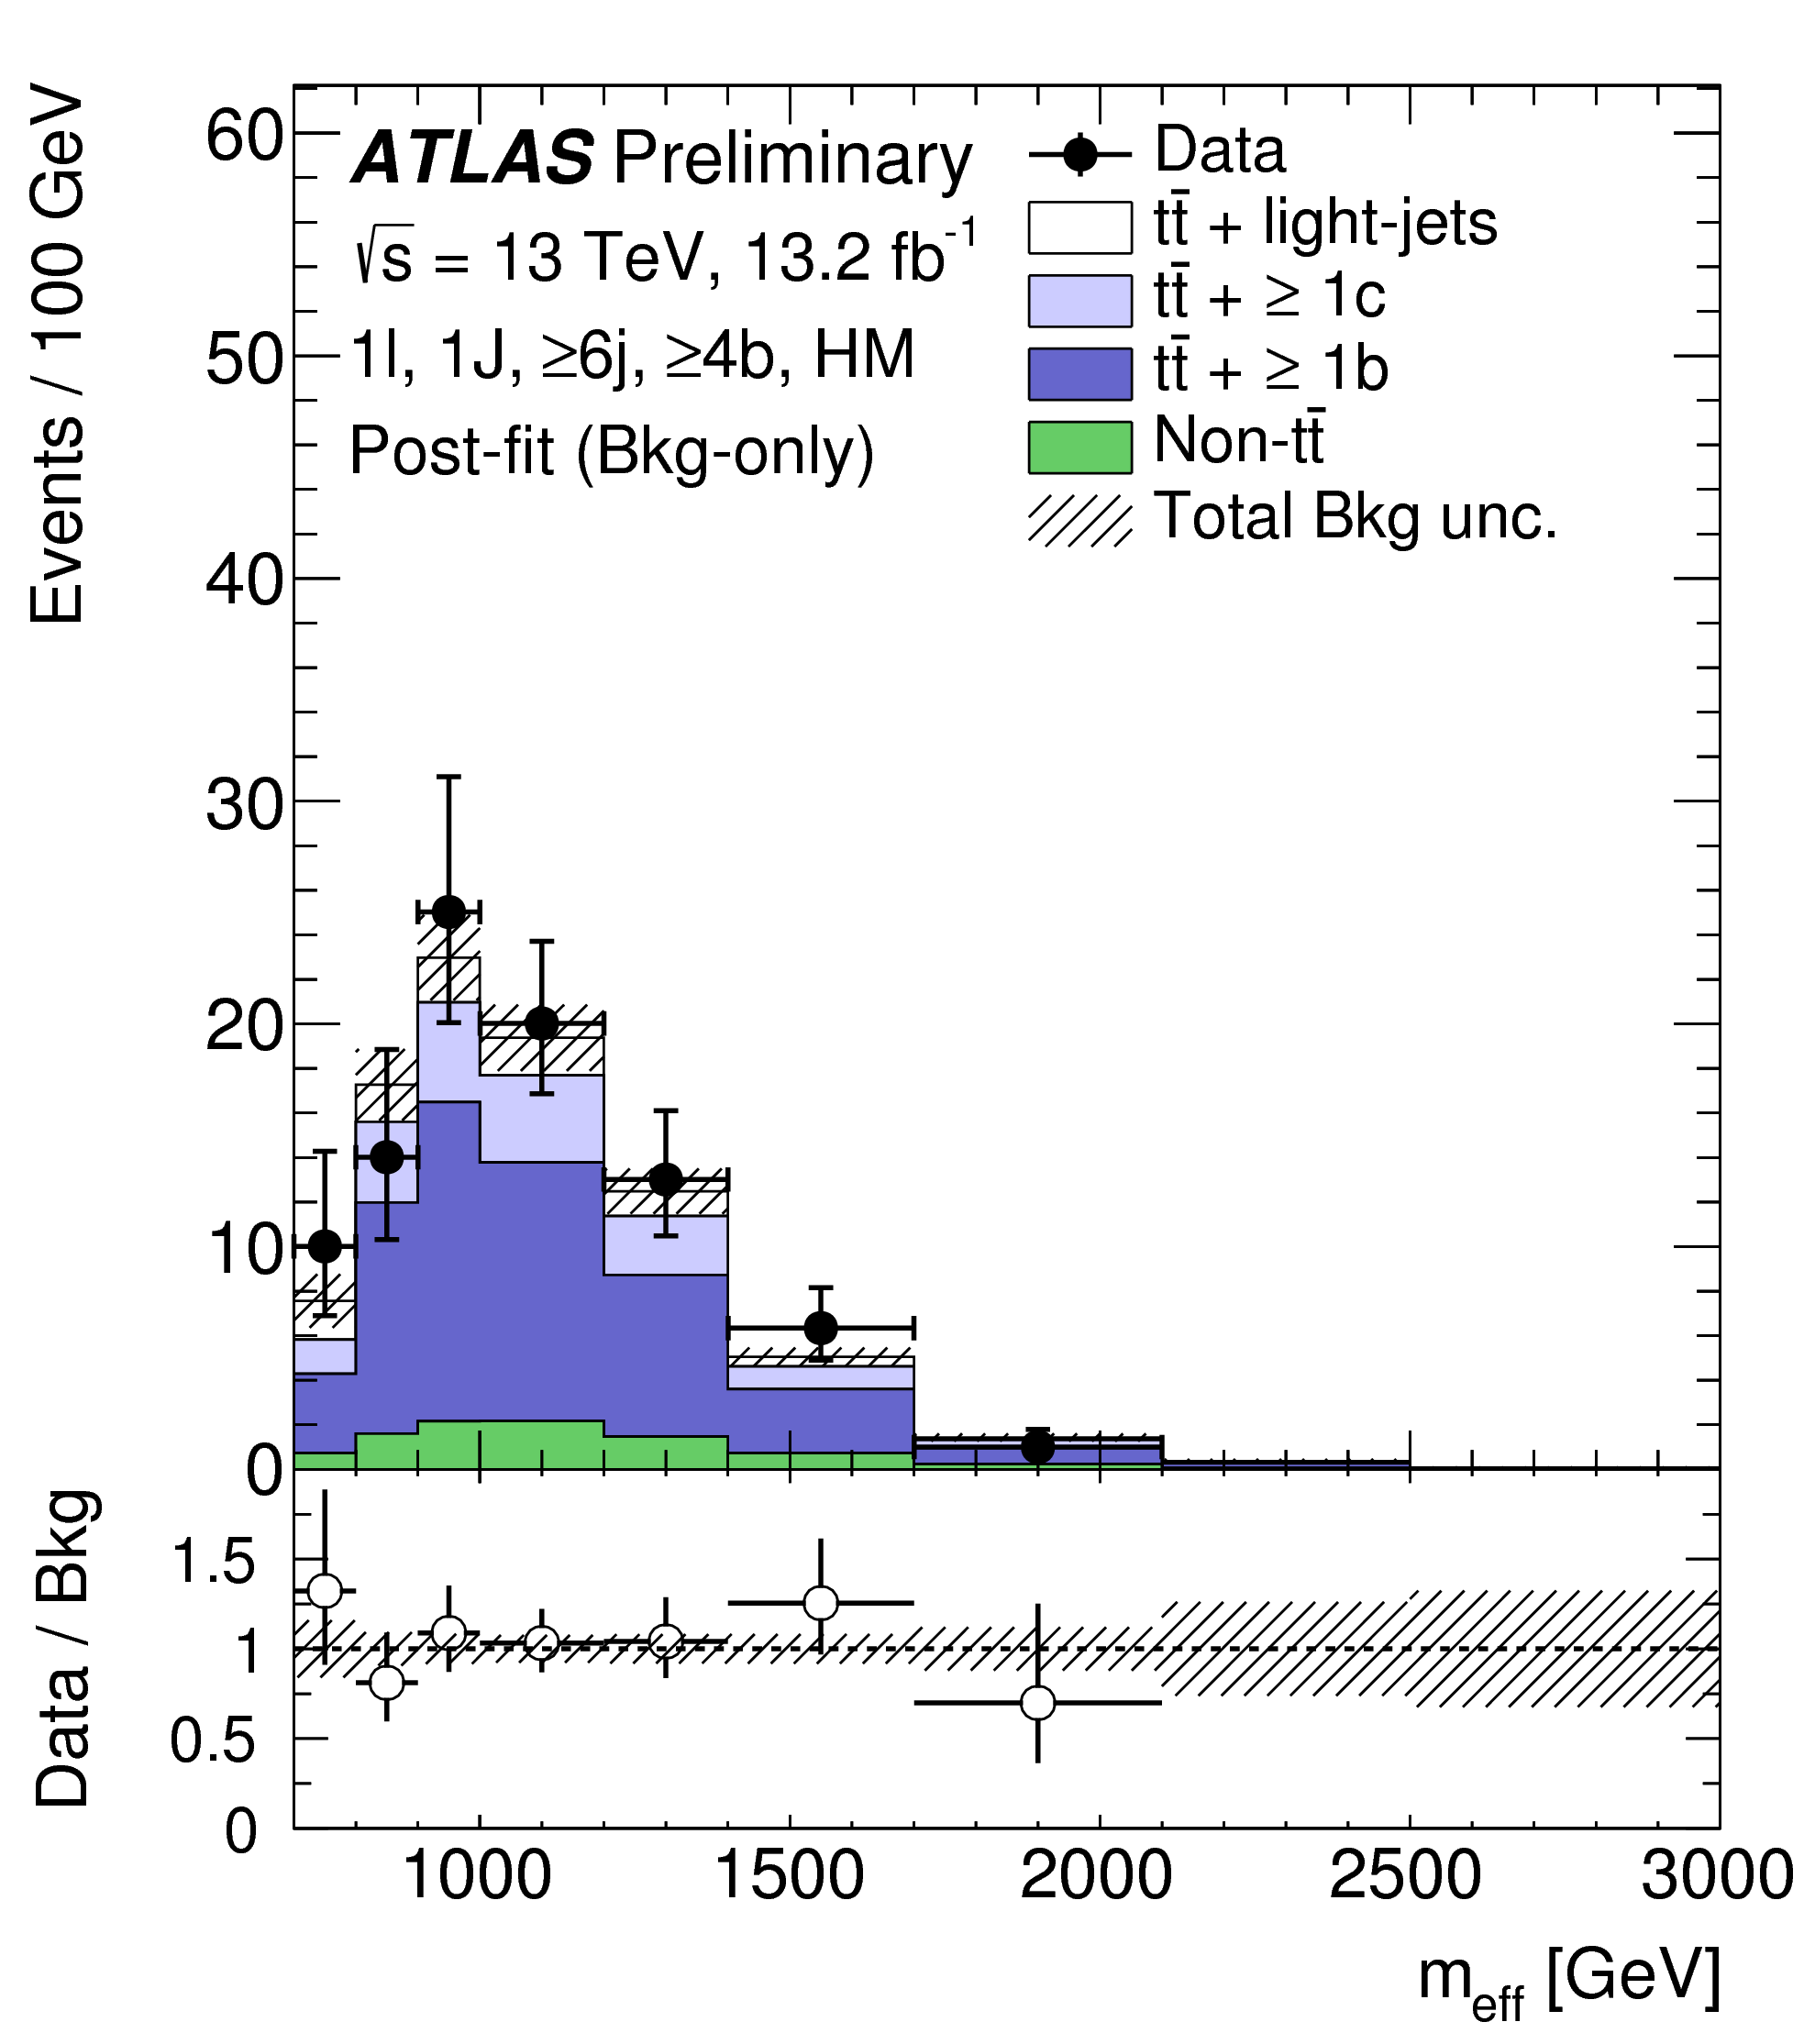
\includegraphics[width=0.9\textwidth]{figures/VLQ/fig_11b.png}
  \caption{}
  \label{}
\end{subfigure}
\begin{subfigure}{0.24\textwidth}
  \centering
  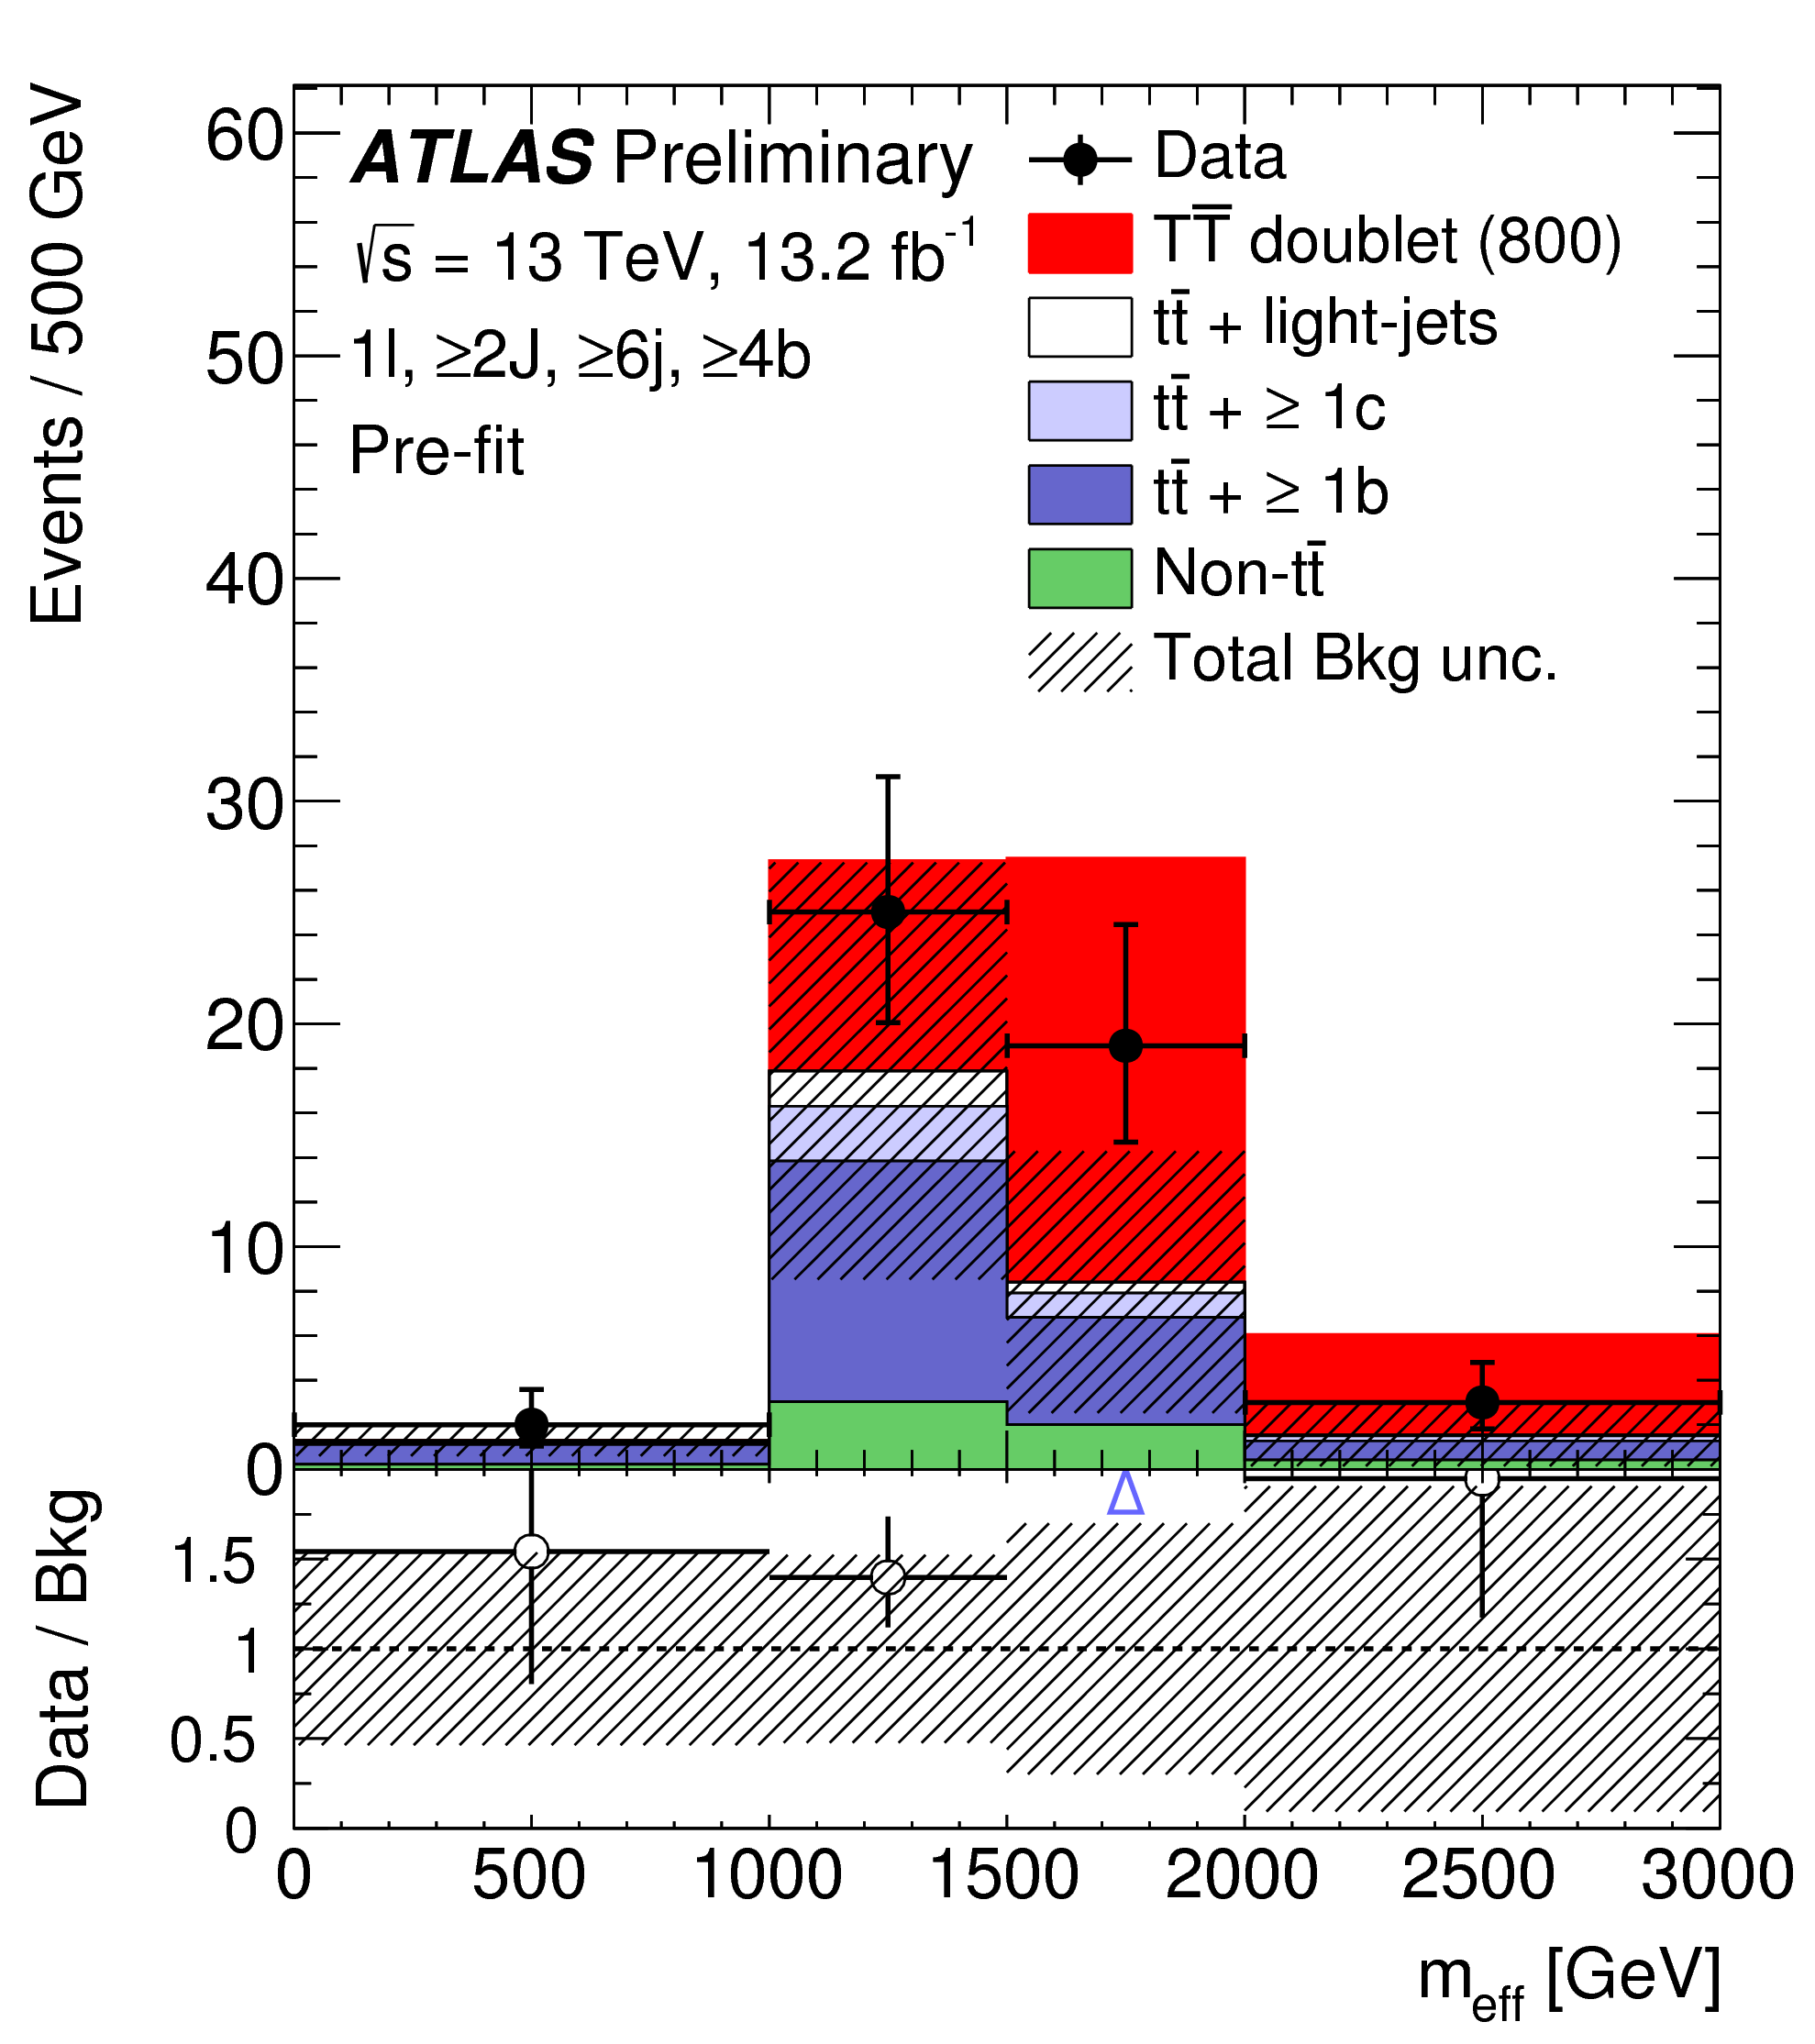
\includegraphics[width=0.9\textwidth]{figures/VLQ/fig_11c.png}
  \caption{}
  \label{}
\end{subfigure}
\begin{subfigure}{0.24\textwidth}
  \centering
  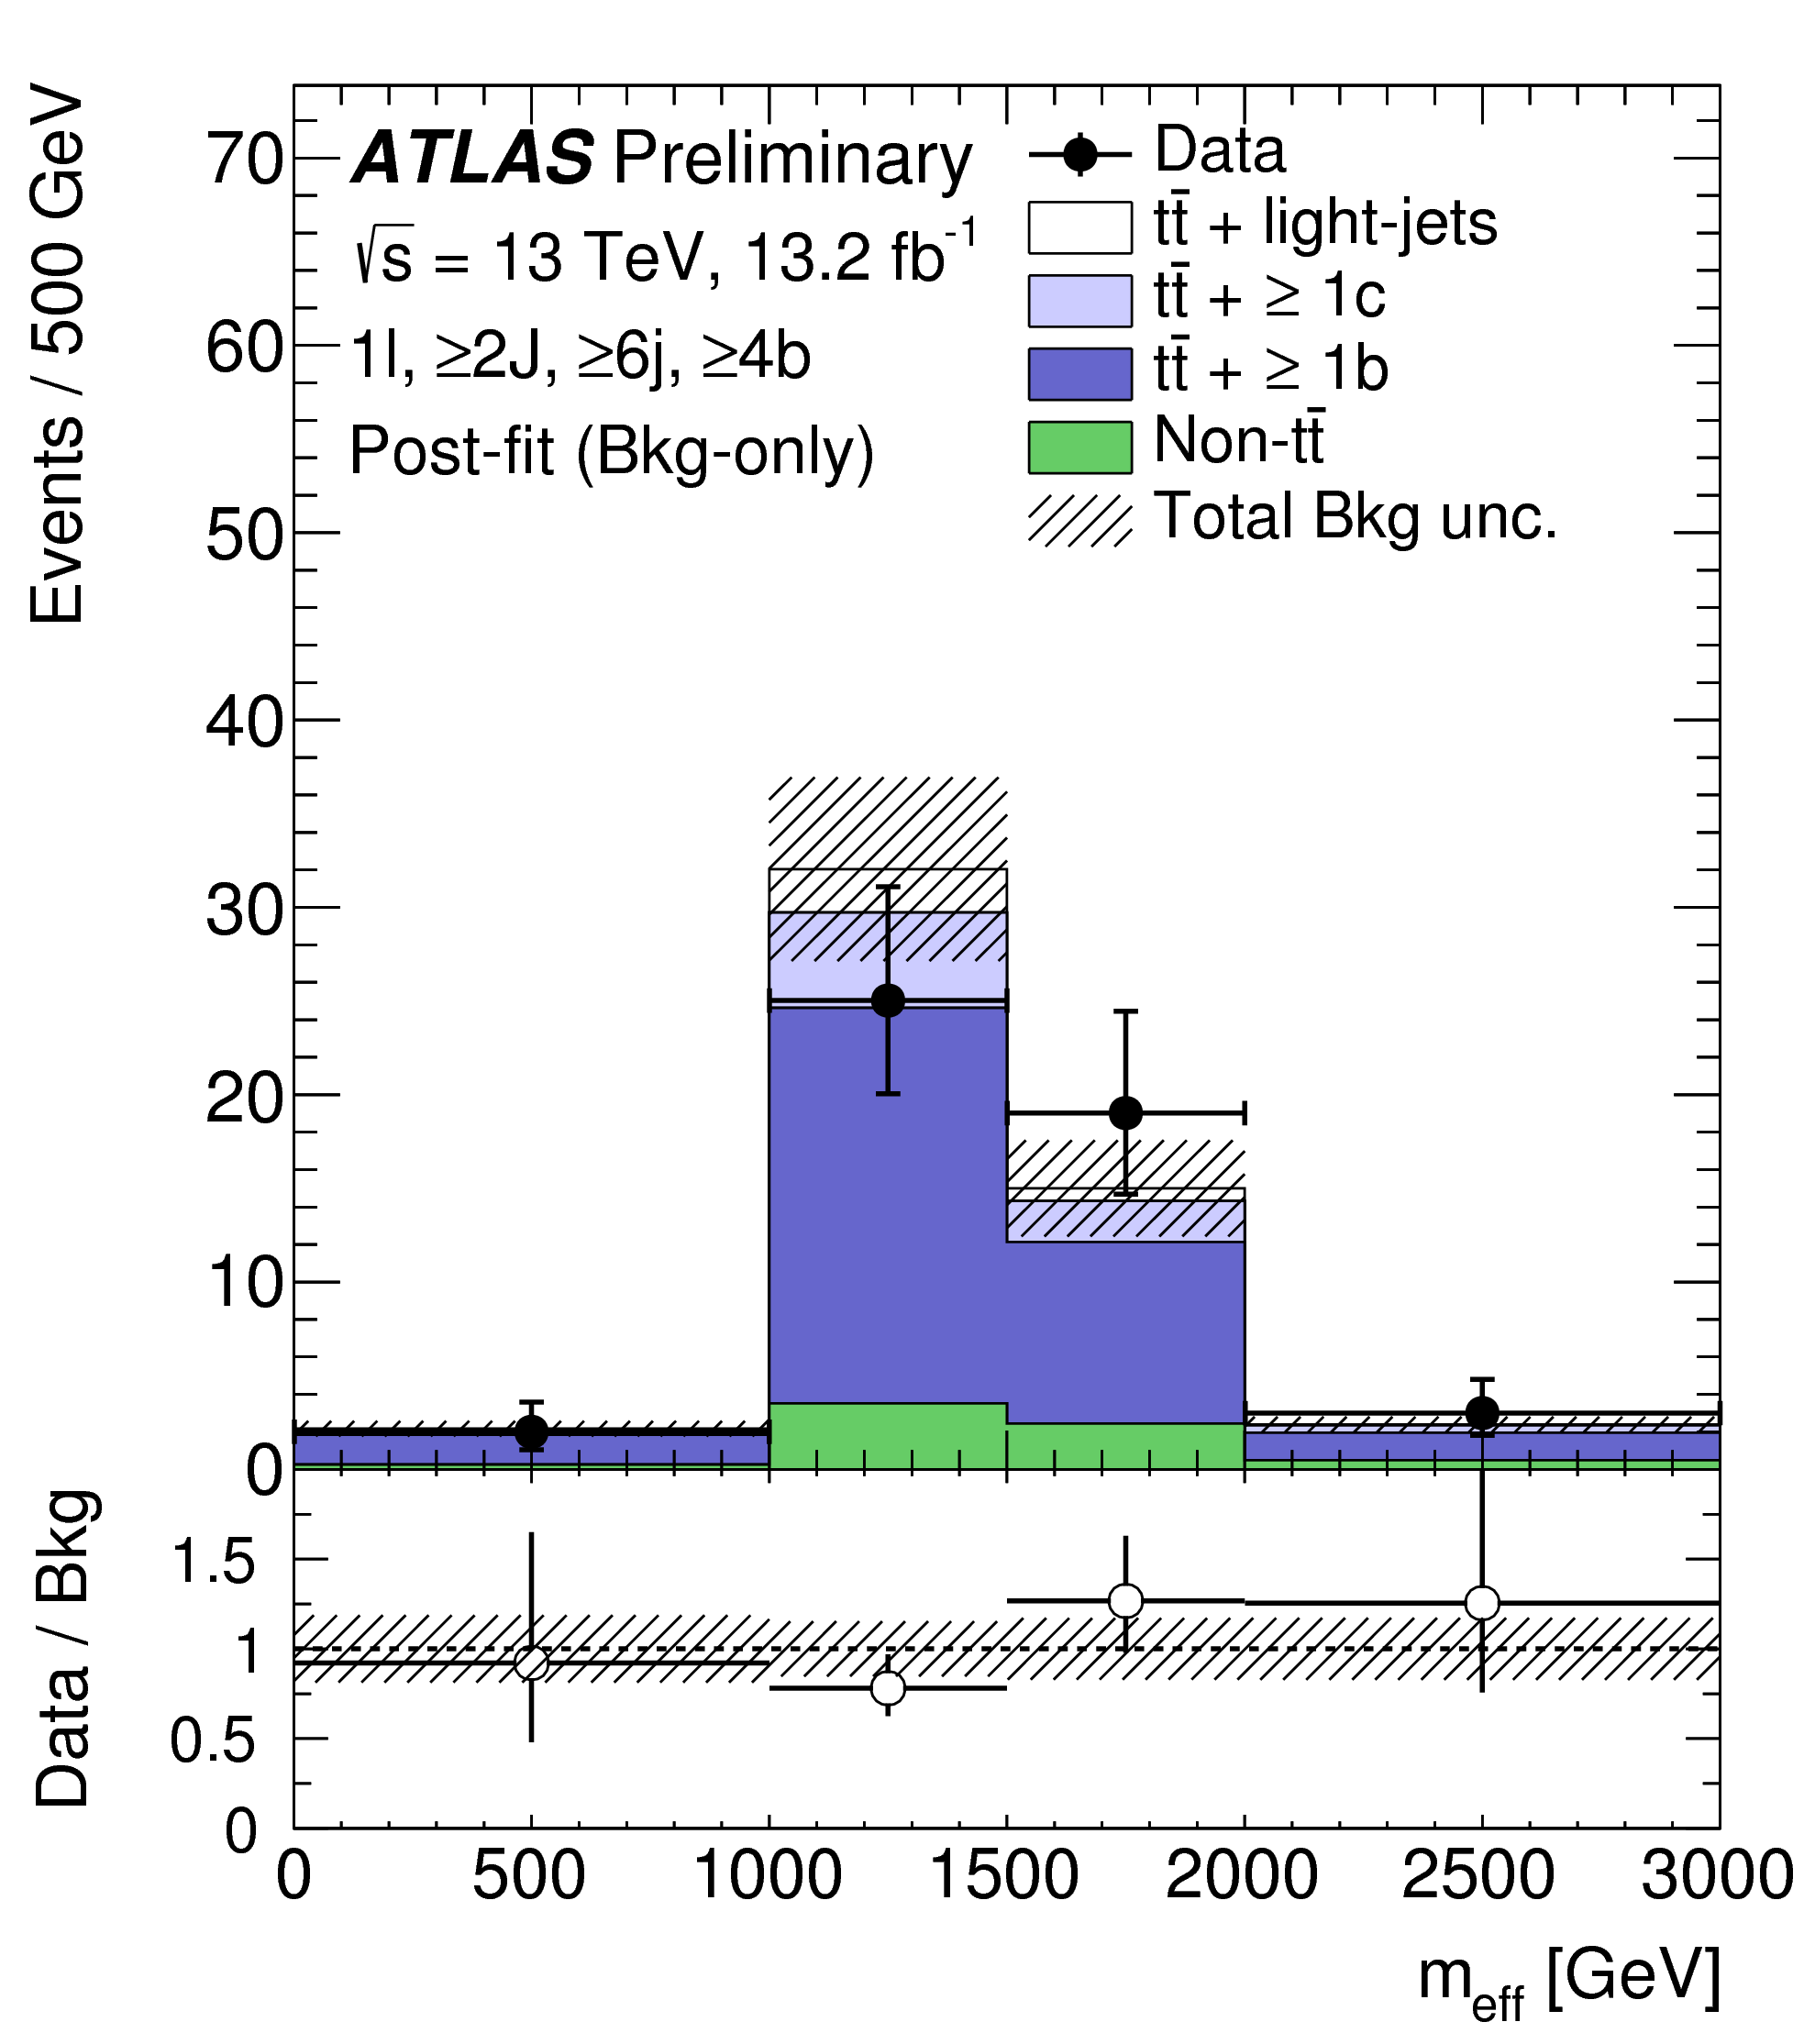
\includegraphics[width=0.9\textwidth]{figures/VLQ/fig_11d.png}
  \caption{}
  \label{}
\end{subfigure}
\captionsetup{width=0.85\textwidth} \caption{\small Comparison between the data and prediction for the $m_{\rm eff}$ distribution in some of the most-sensitive search regions in the 1-lepton channel,
before and after performing the combined fit to data in the 0-lepton and 1-lepton channels (``Pre-fit'' and ``Post-fit'', respectively) under the background-only hypothesis. Shown are the (0J, $\geq$6j, $\geq$4b) region (a) pre-fit and (b) post-fit,  and the (1J, $\geq$6j, $\geq$4b, LM) region (c) pre-fit and (d) post-fit, (1J, $\geq$6j, $\geq$4b, HM) region (e) pre-fit and (f) post-fit,  and the ($\geq$2J, $\geq$6j, $\geq$4b) region (g) pre-fit and (h) post-fit.
In the pre-fit figures the expected $T\bar{T}$ signal (solid red) corresponding to $m_{T}=800$ $\gev$ in the doublet $T$-quark scenario is also shown, added on top of the background prediction. The small contributions from $t\bar{t}V$, $t\bar{t} H$, single top, $W/Z$+jets, diboson, and multijet backgrounds are combined into a single background source  referred to as ``Non-$t\bar{t}$''. The last bin in all figures contains the overflow. The bottom panels display the ratios of data to the total background prediction (``Bkg''). The blue triangles indicate points that are outside the vertical range of the figure. The hashed area represents the total uncertainty on the background. In the case of the pre-fit background uncertainty, the normalisation uncertainty on the $t\bar{t}+\ge1b$ background is not included.}
\label{sec:vlq:fig:meff1}
\end{figure}


\begin{figure}[p!]
\begin{subfigure}{0.24\textwidth}
  \centering
  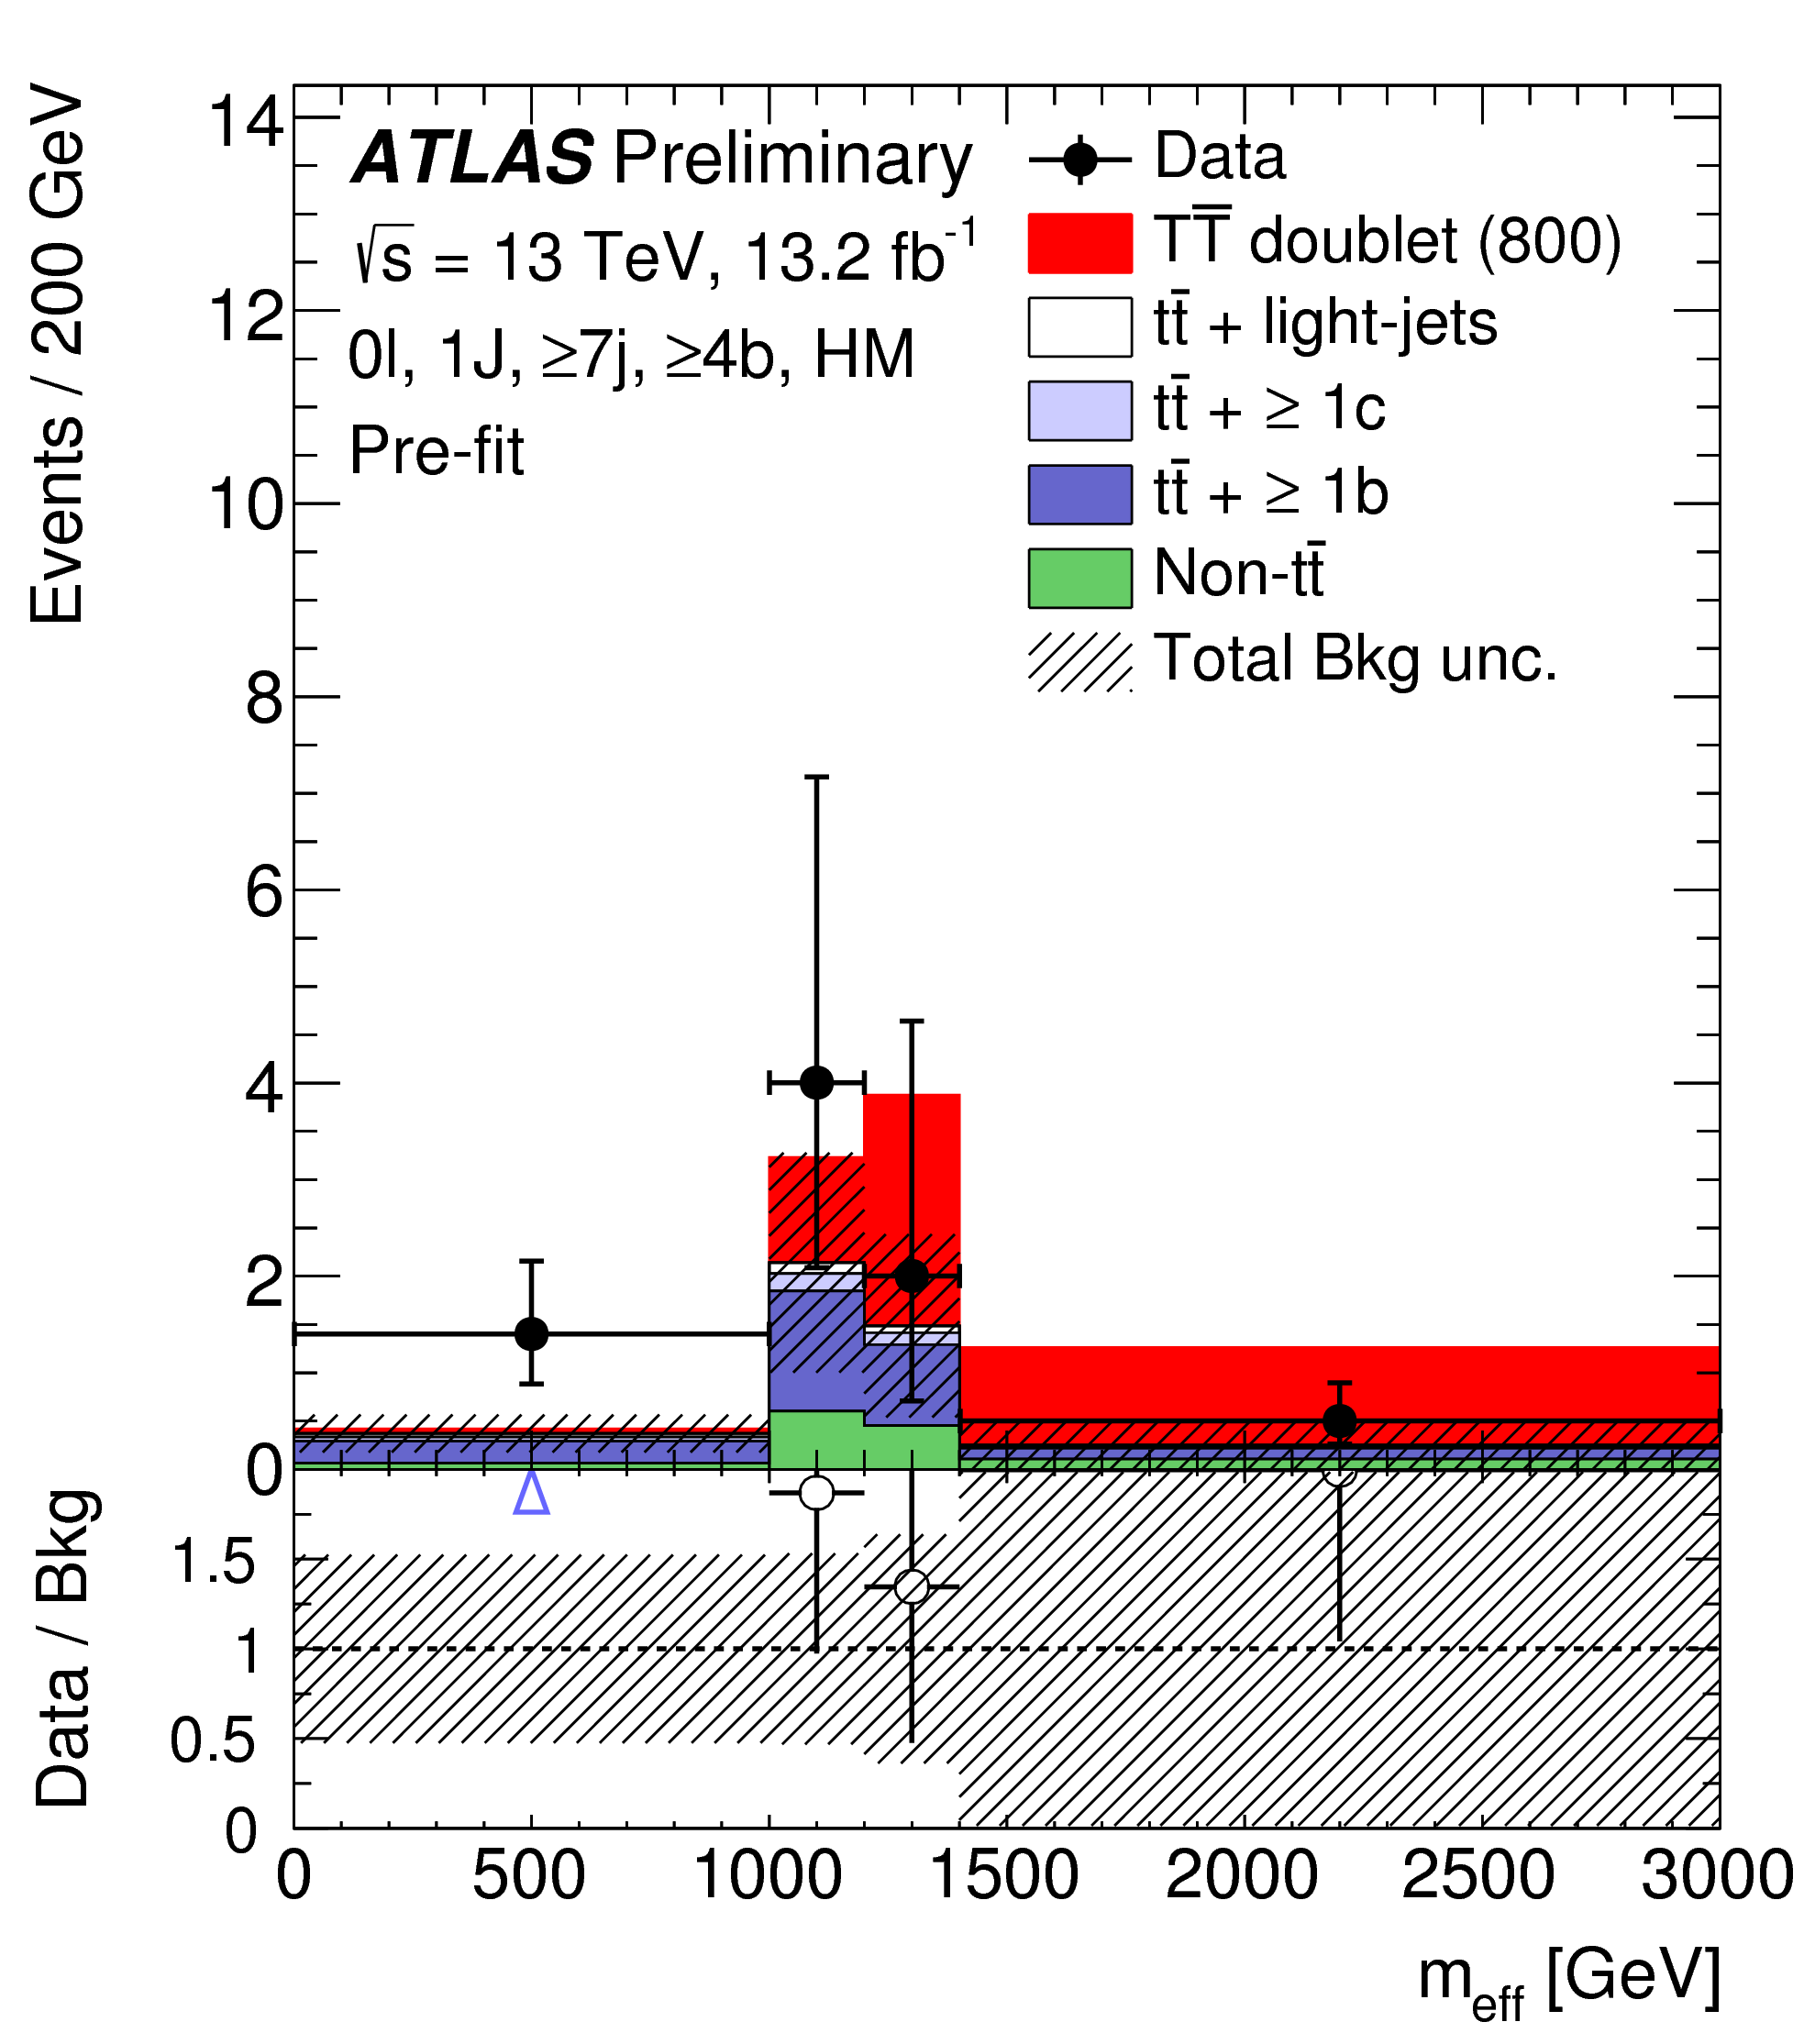
\includegraphics[width=0.9\textwidth]{figures/VLQ/fig_12a.png}
  \caption{}
  \label{}
\end{subfigure}
\begin{subfigure}{0.24\textwidth}
  \centering
  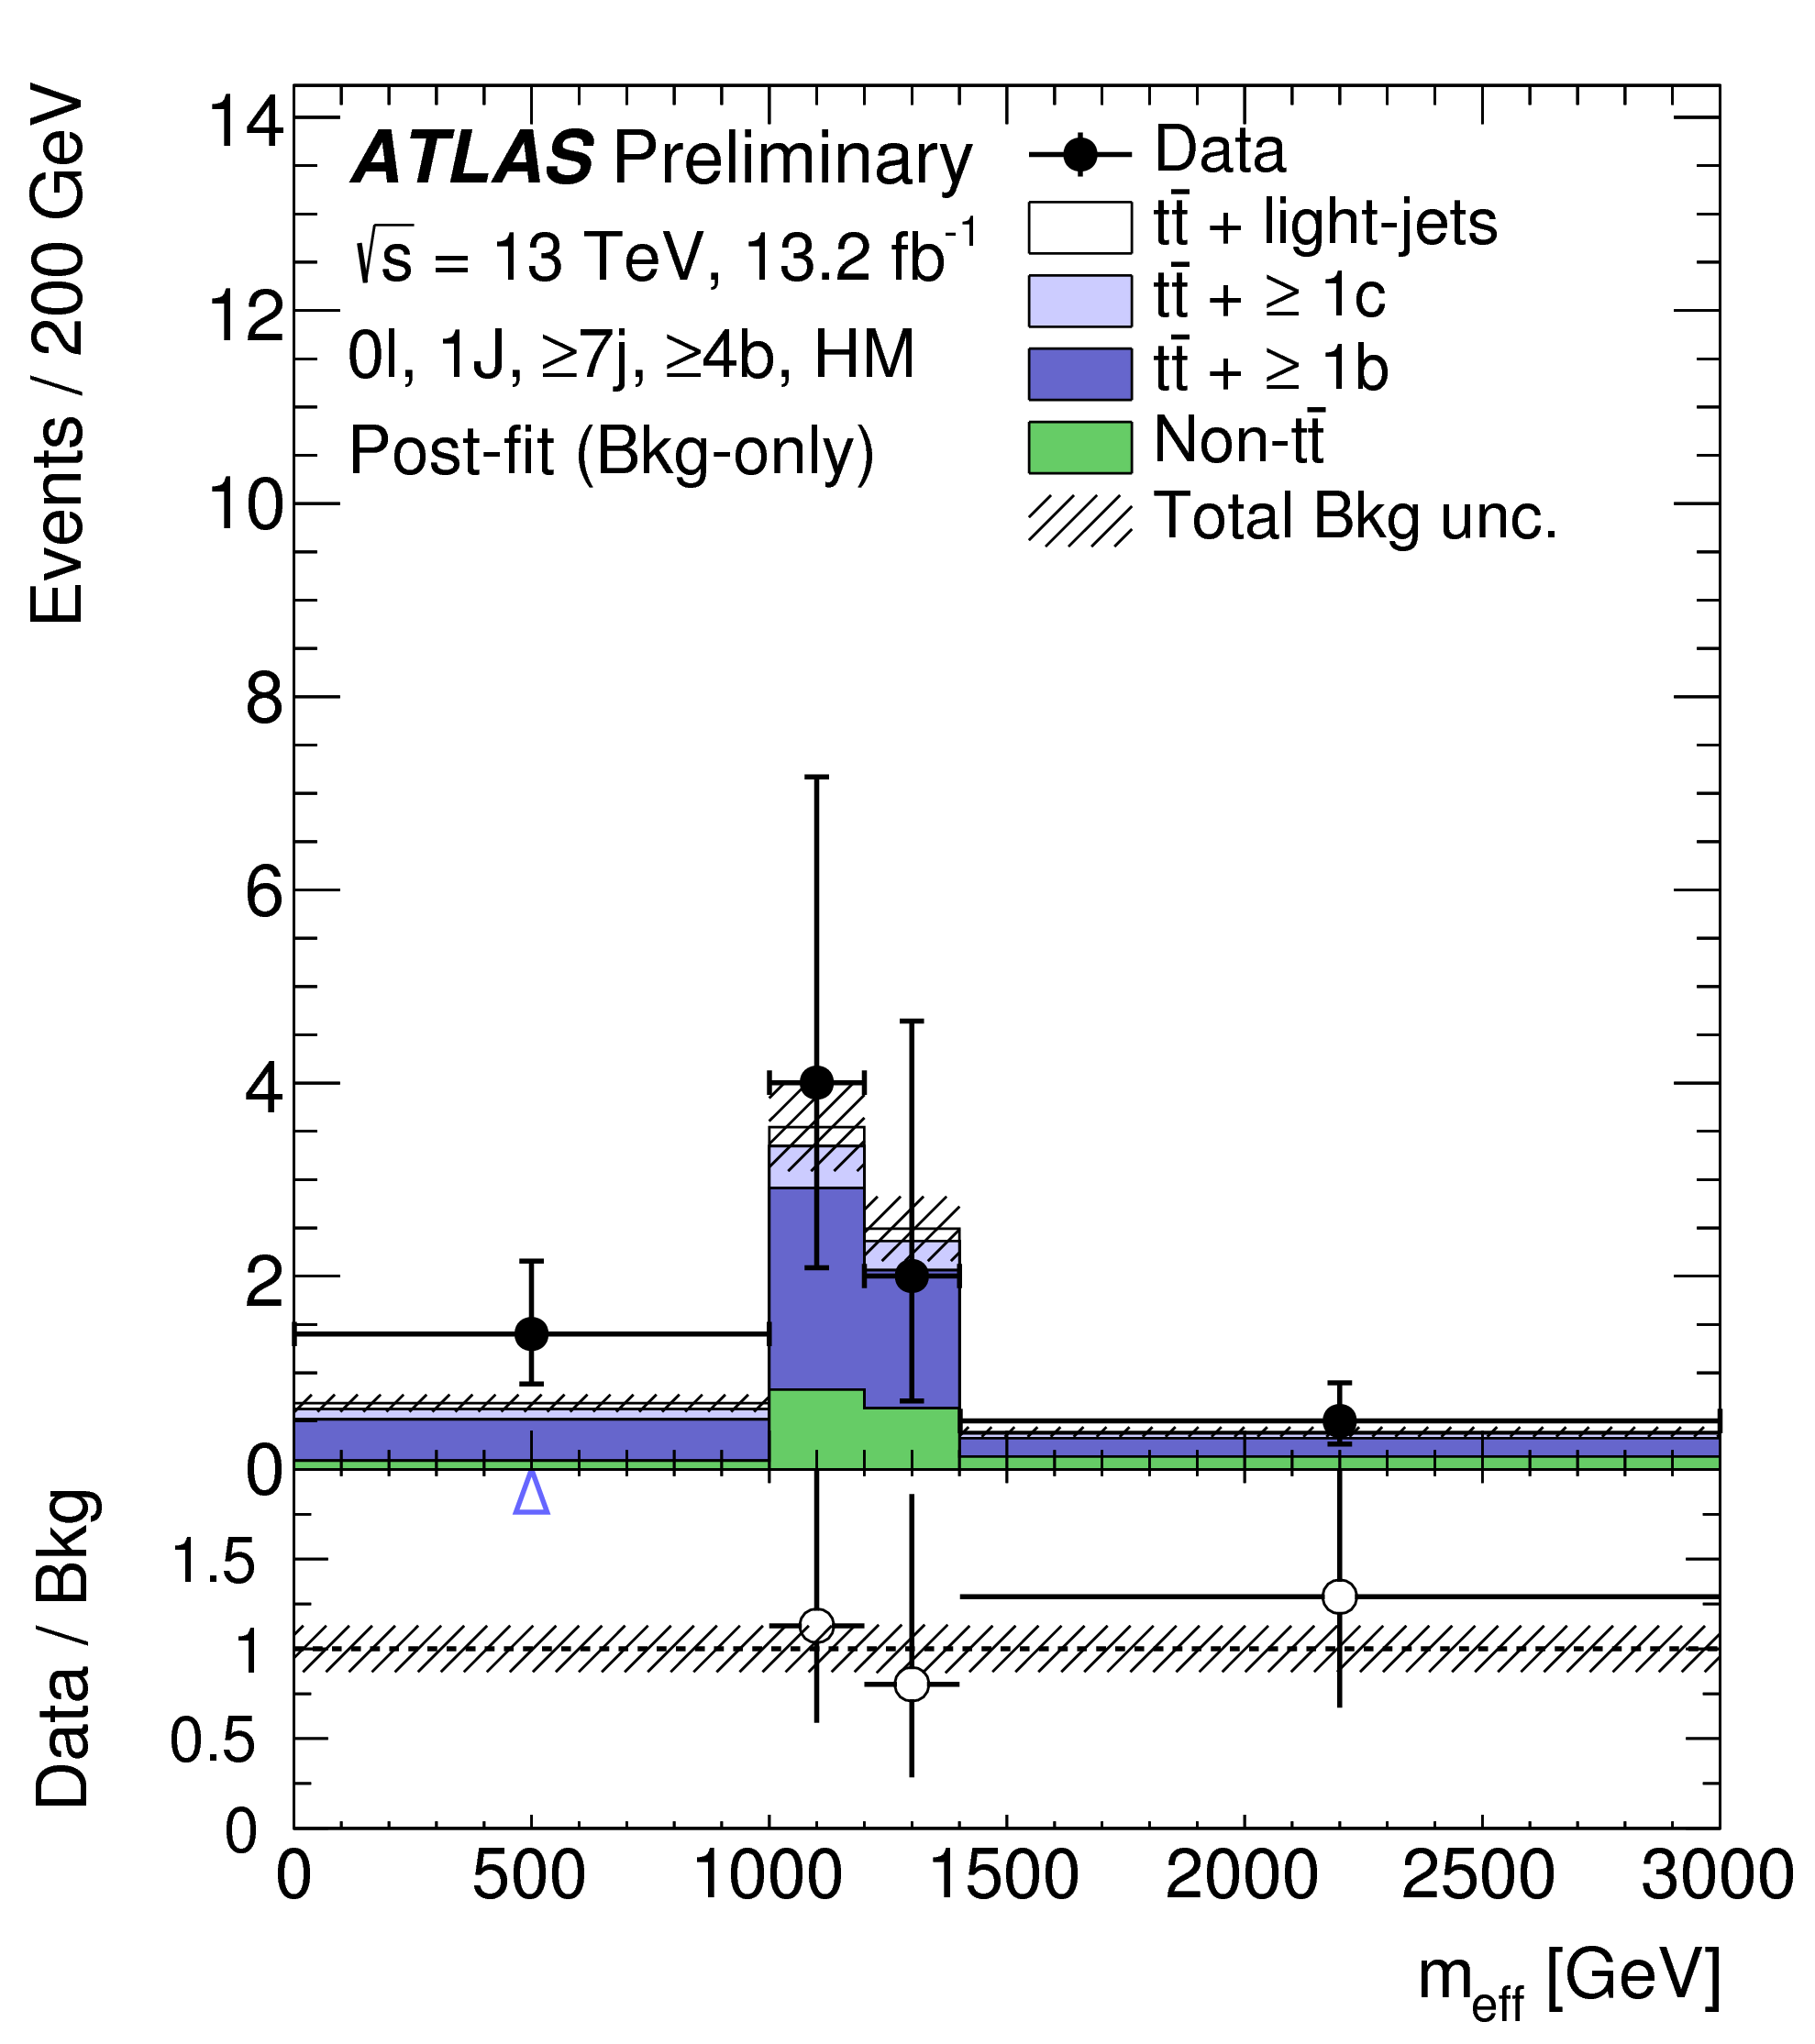
\includegraphics[width=0.9\textwidth]{figures/VLQ/fig_12b.png}
  \caption{}
  \label{}
\end{subfigure}
\begin{subfigure}{0.24\textwidth}
  \centering
  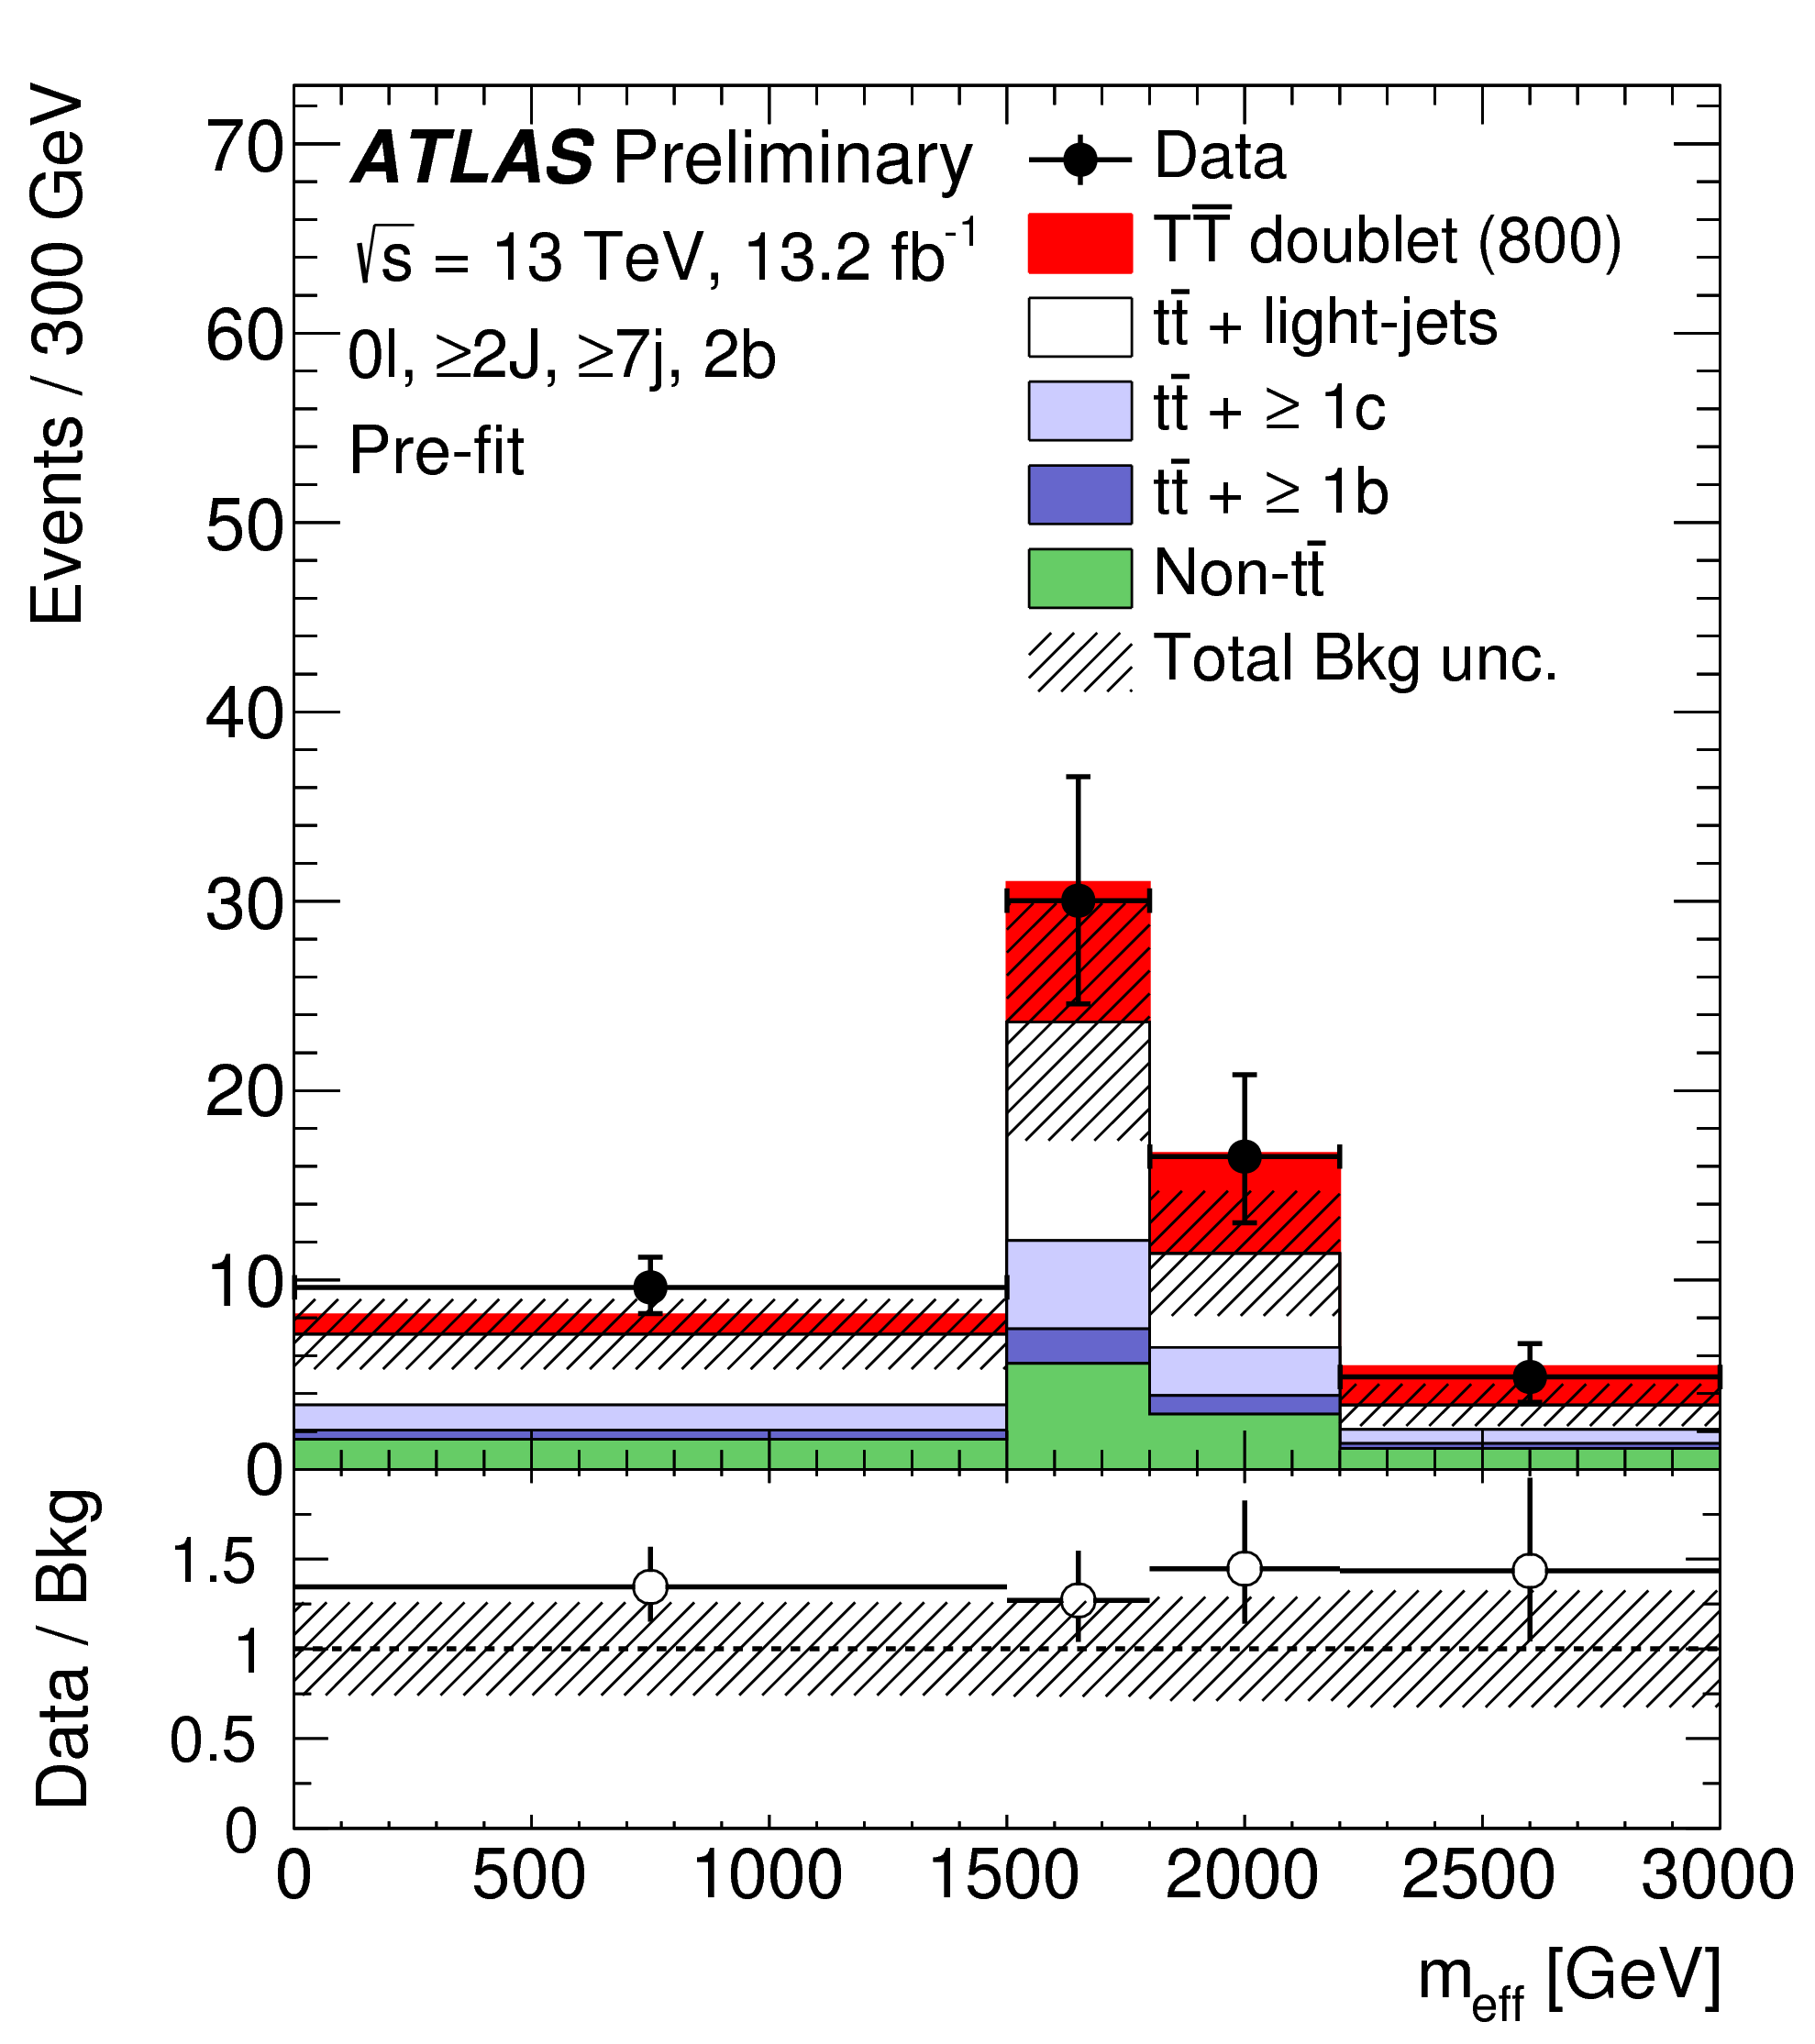
\includegraphics[width=0.9\textwidth]{figures/VLQ/fig_12c.png}
  \caption{}
  \label{}
\end{subfigure}
\begin{subfigure}{0.24\textwidth}
  \centering
  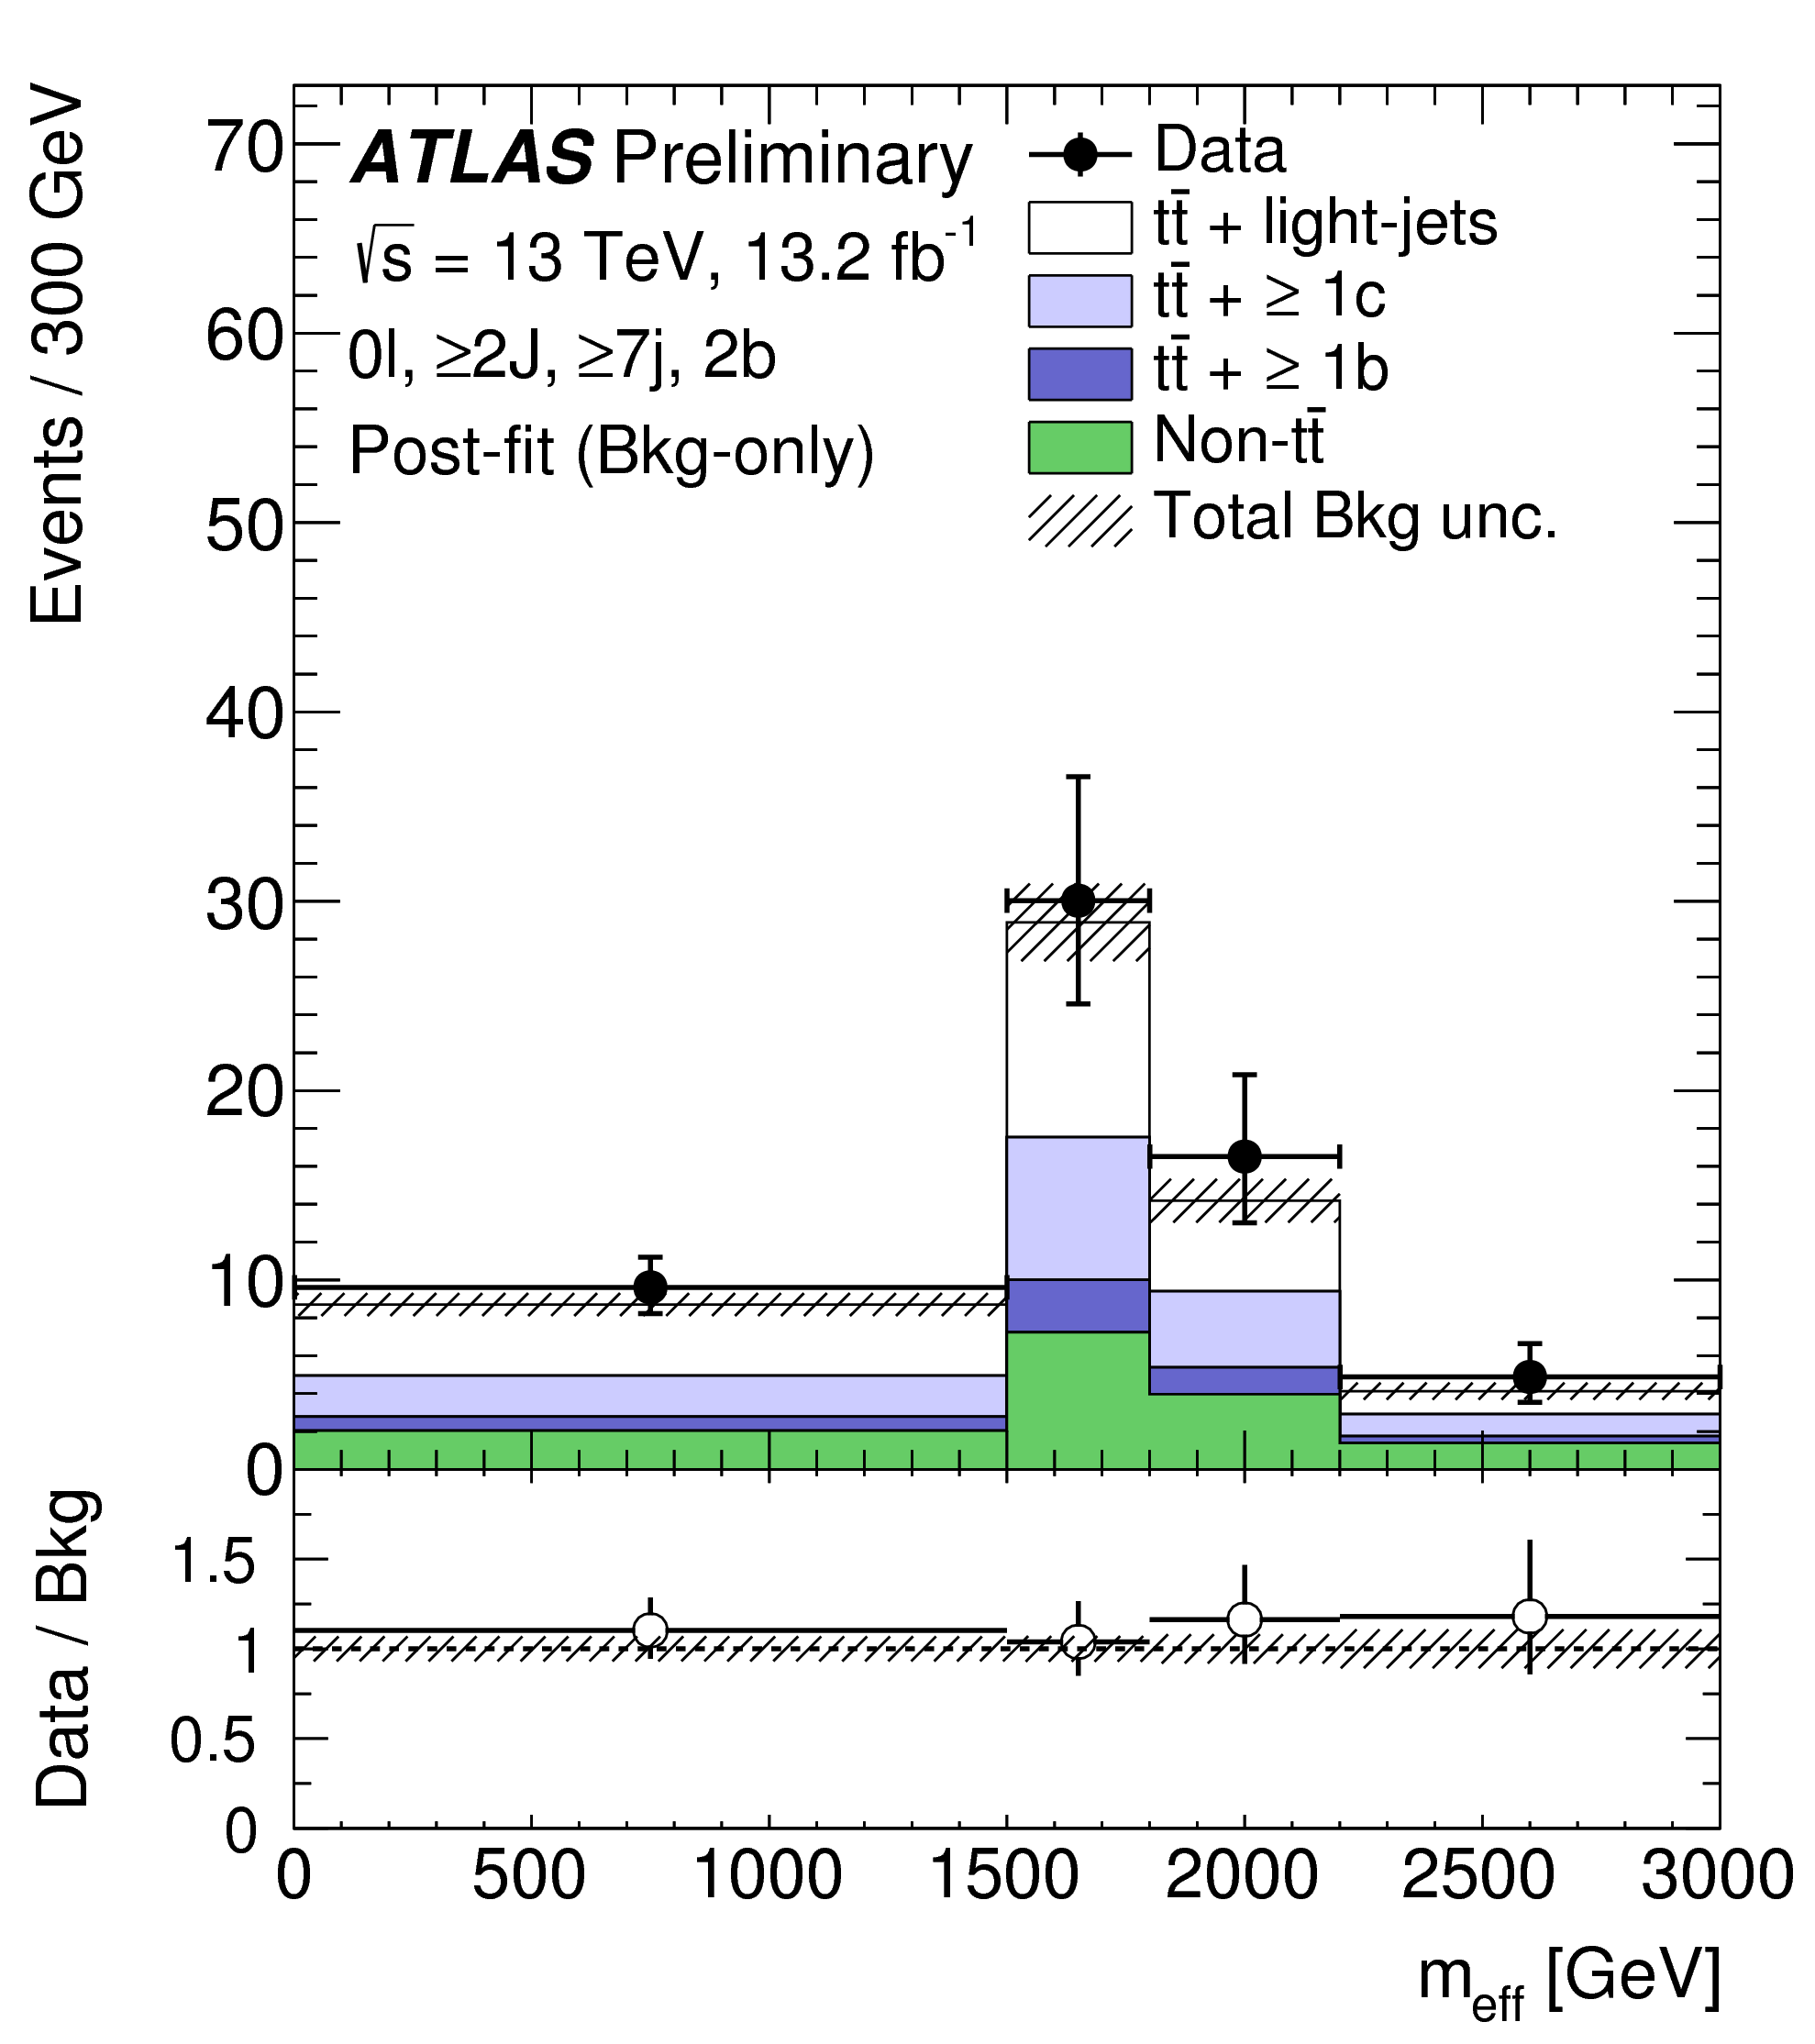
\includegraphics[width=0.9\textwidth]{figures/VLQ/fig_12d.png}
  \caption{}
  \label{}
\end{subfigure}
\begin{subfigure}{0.24\textwidth}
  \centering
  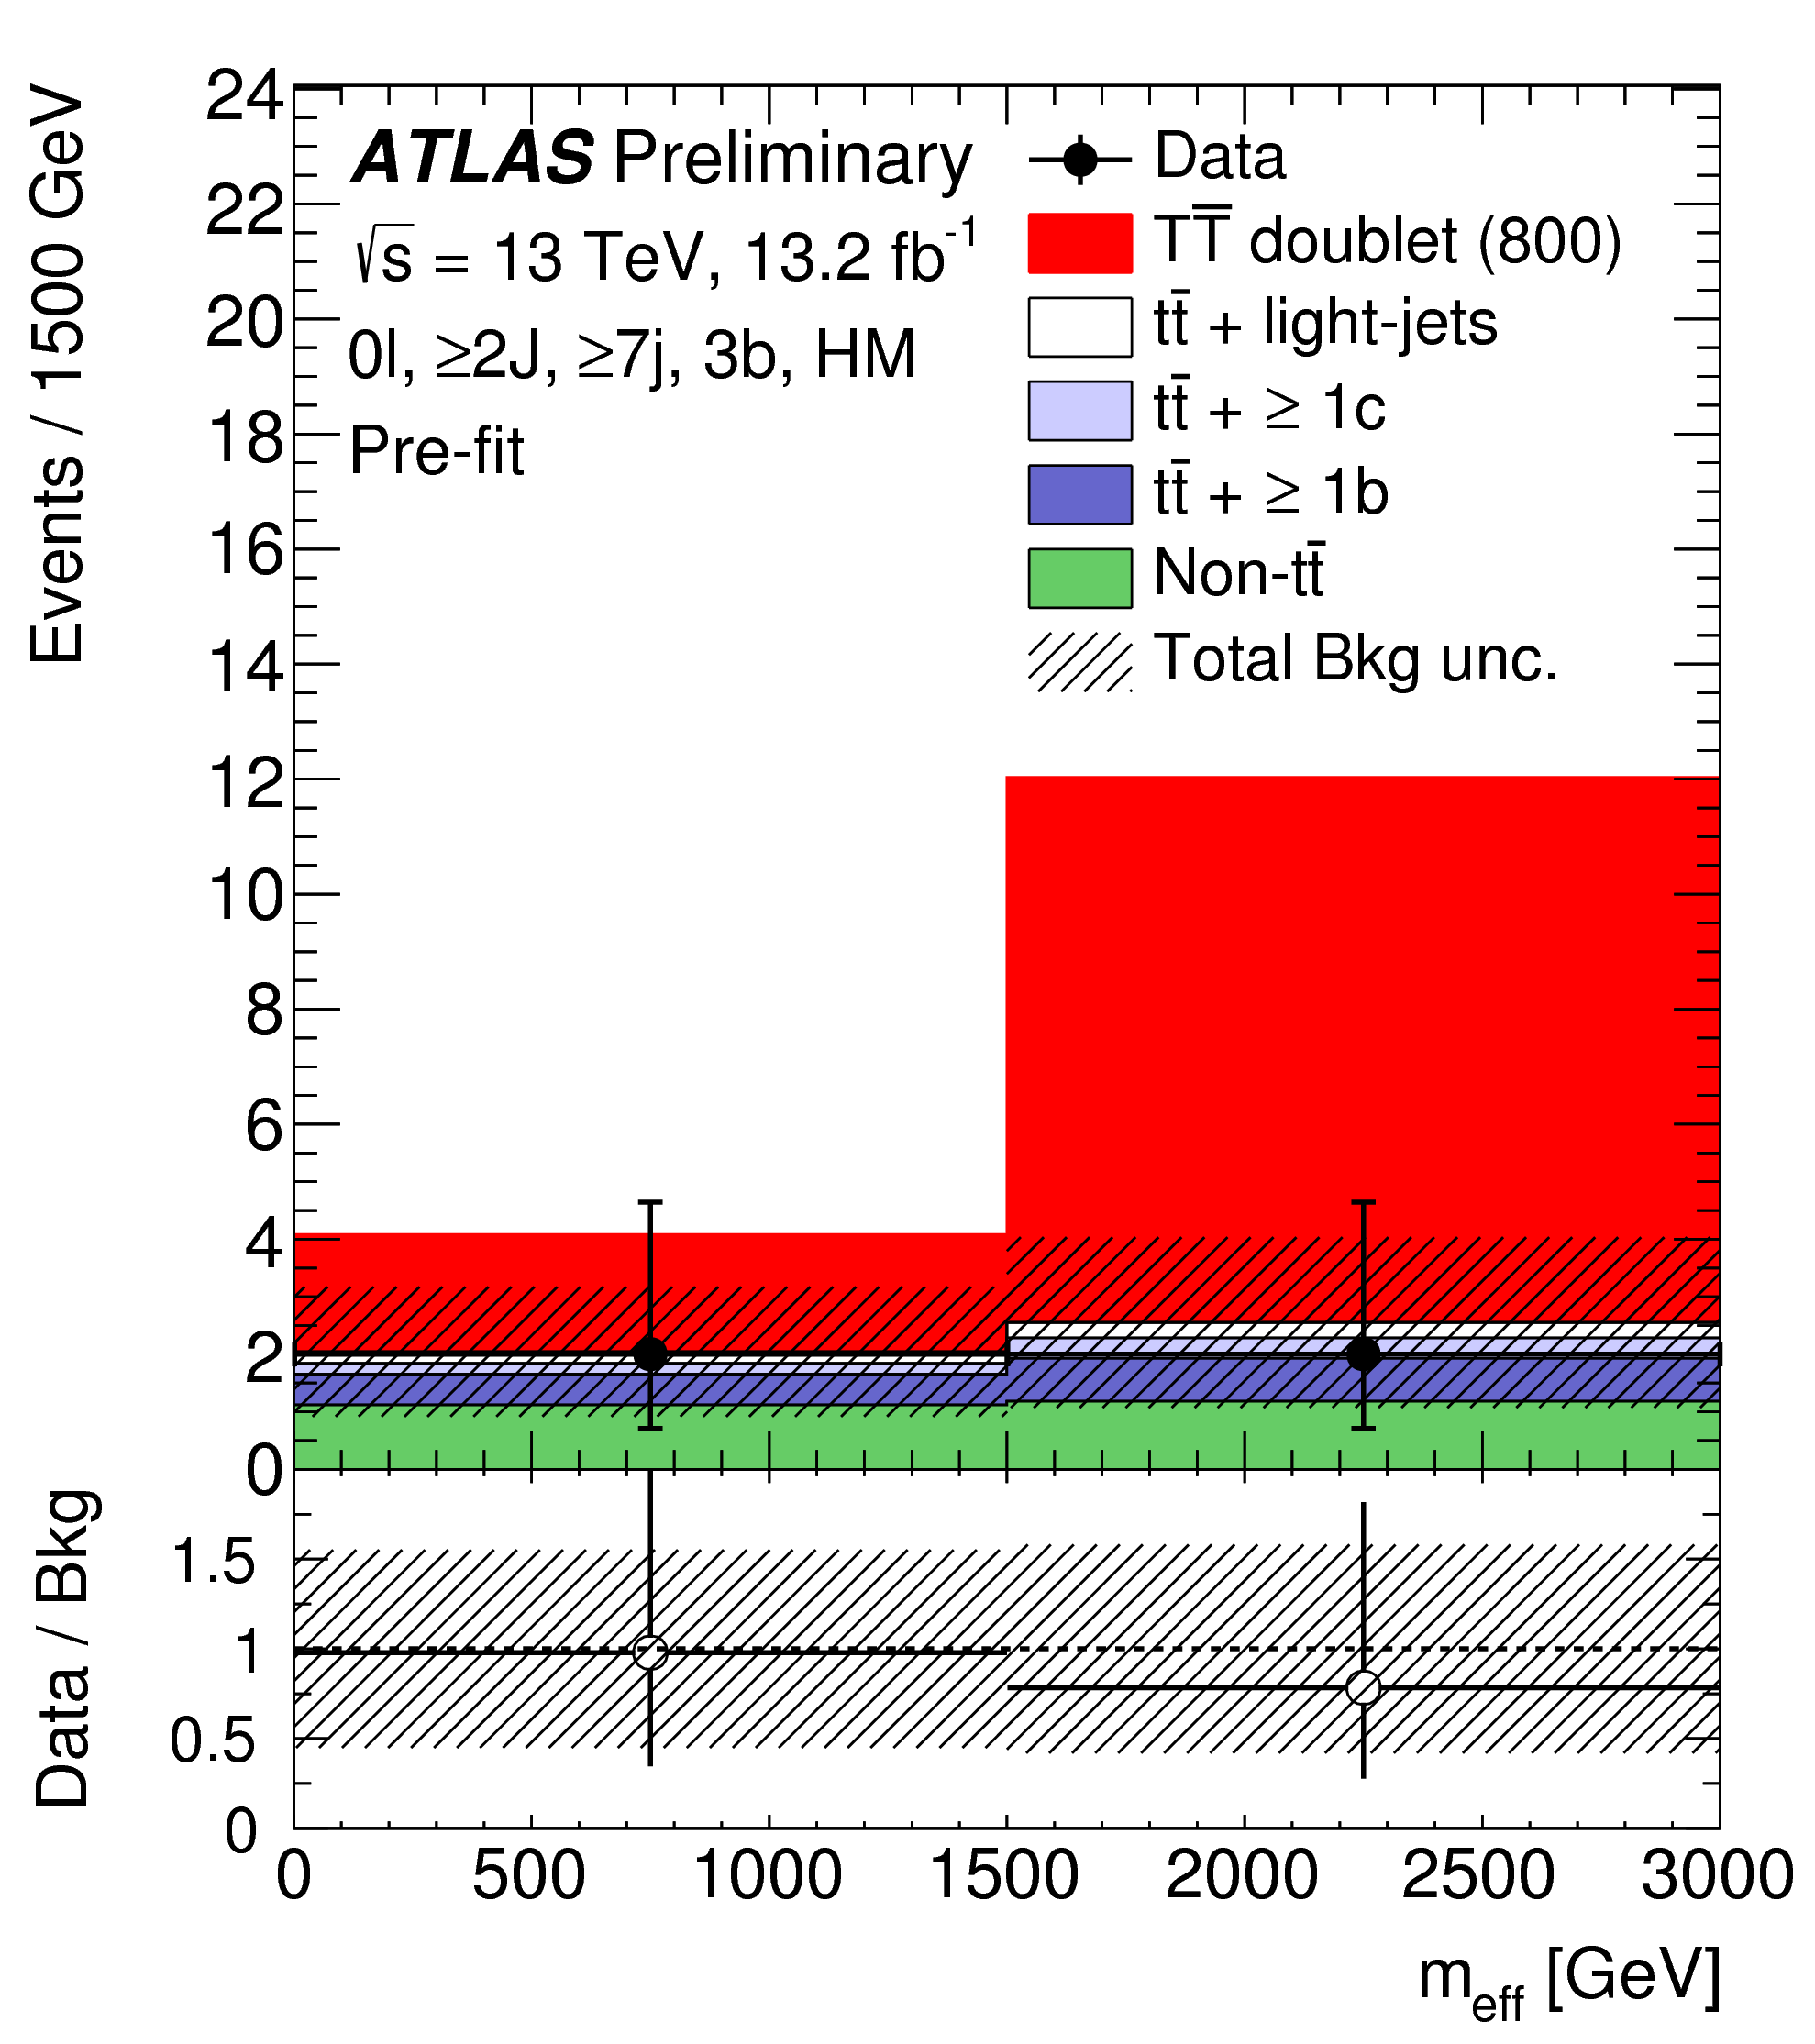
\includegraphics[width=0.9\textwidth]{figures/VLQ/fig_13a.png}
  \caption{}
  \label{}
\end{subfigure}
\begin{subfigure}{0.24\textwidth}
  \centering
  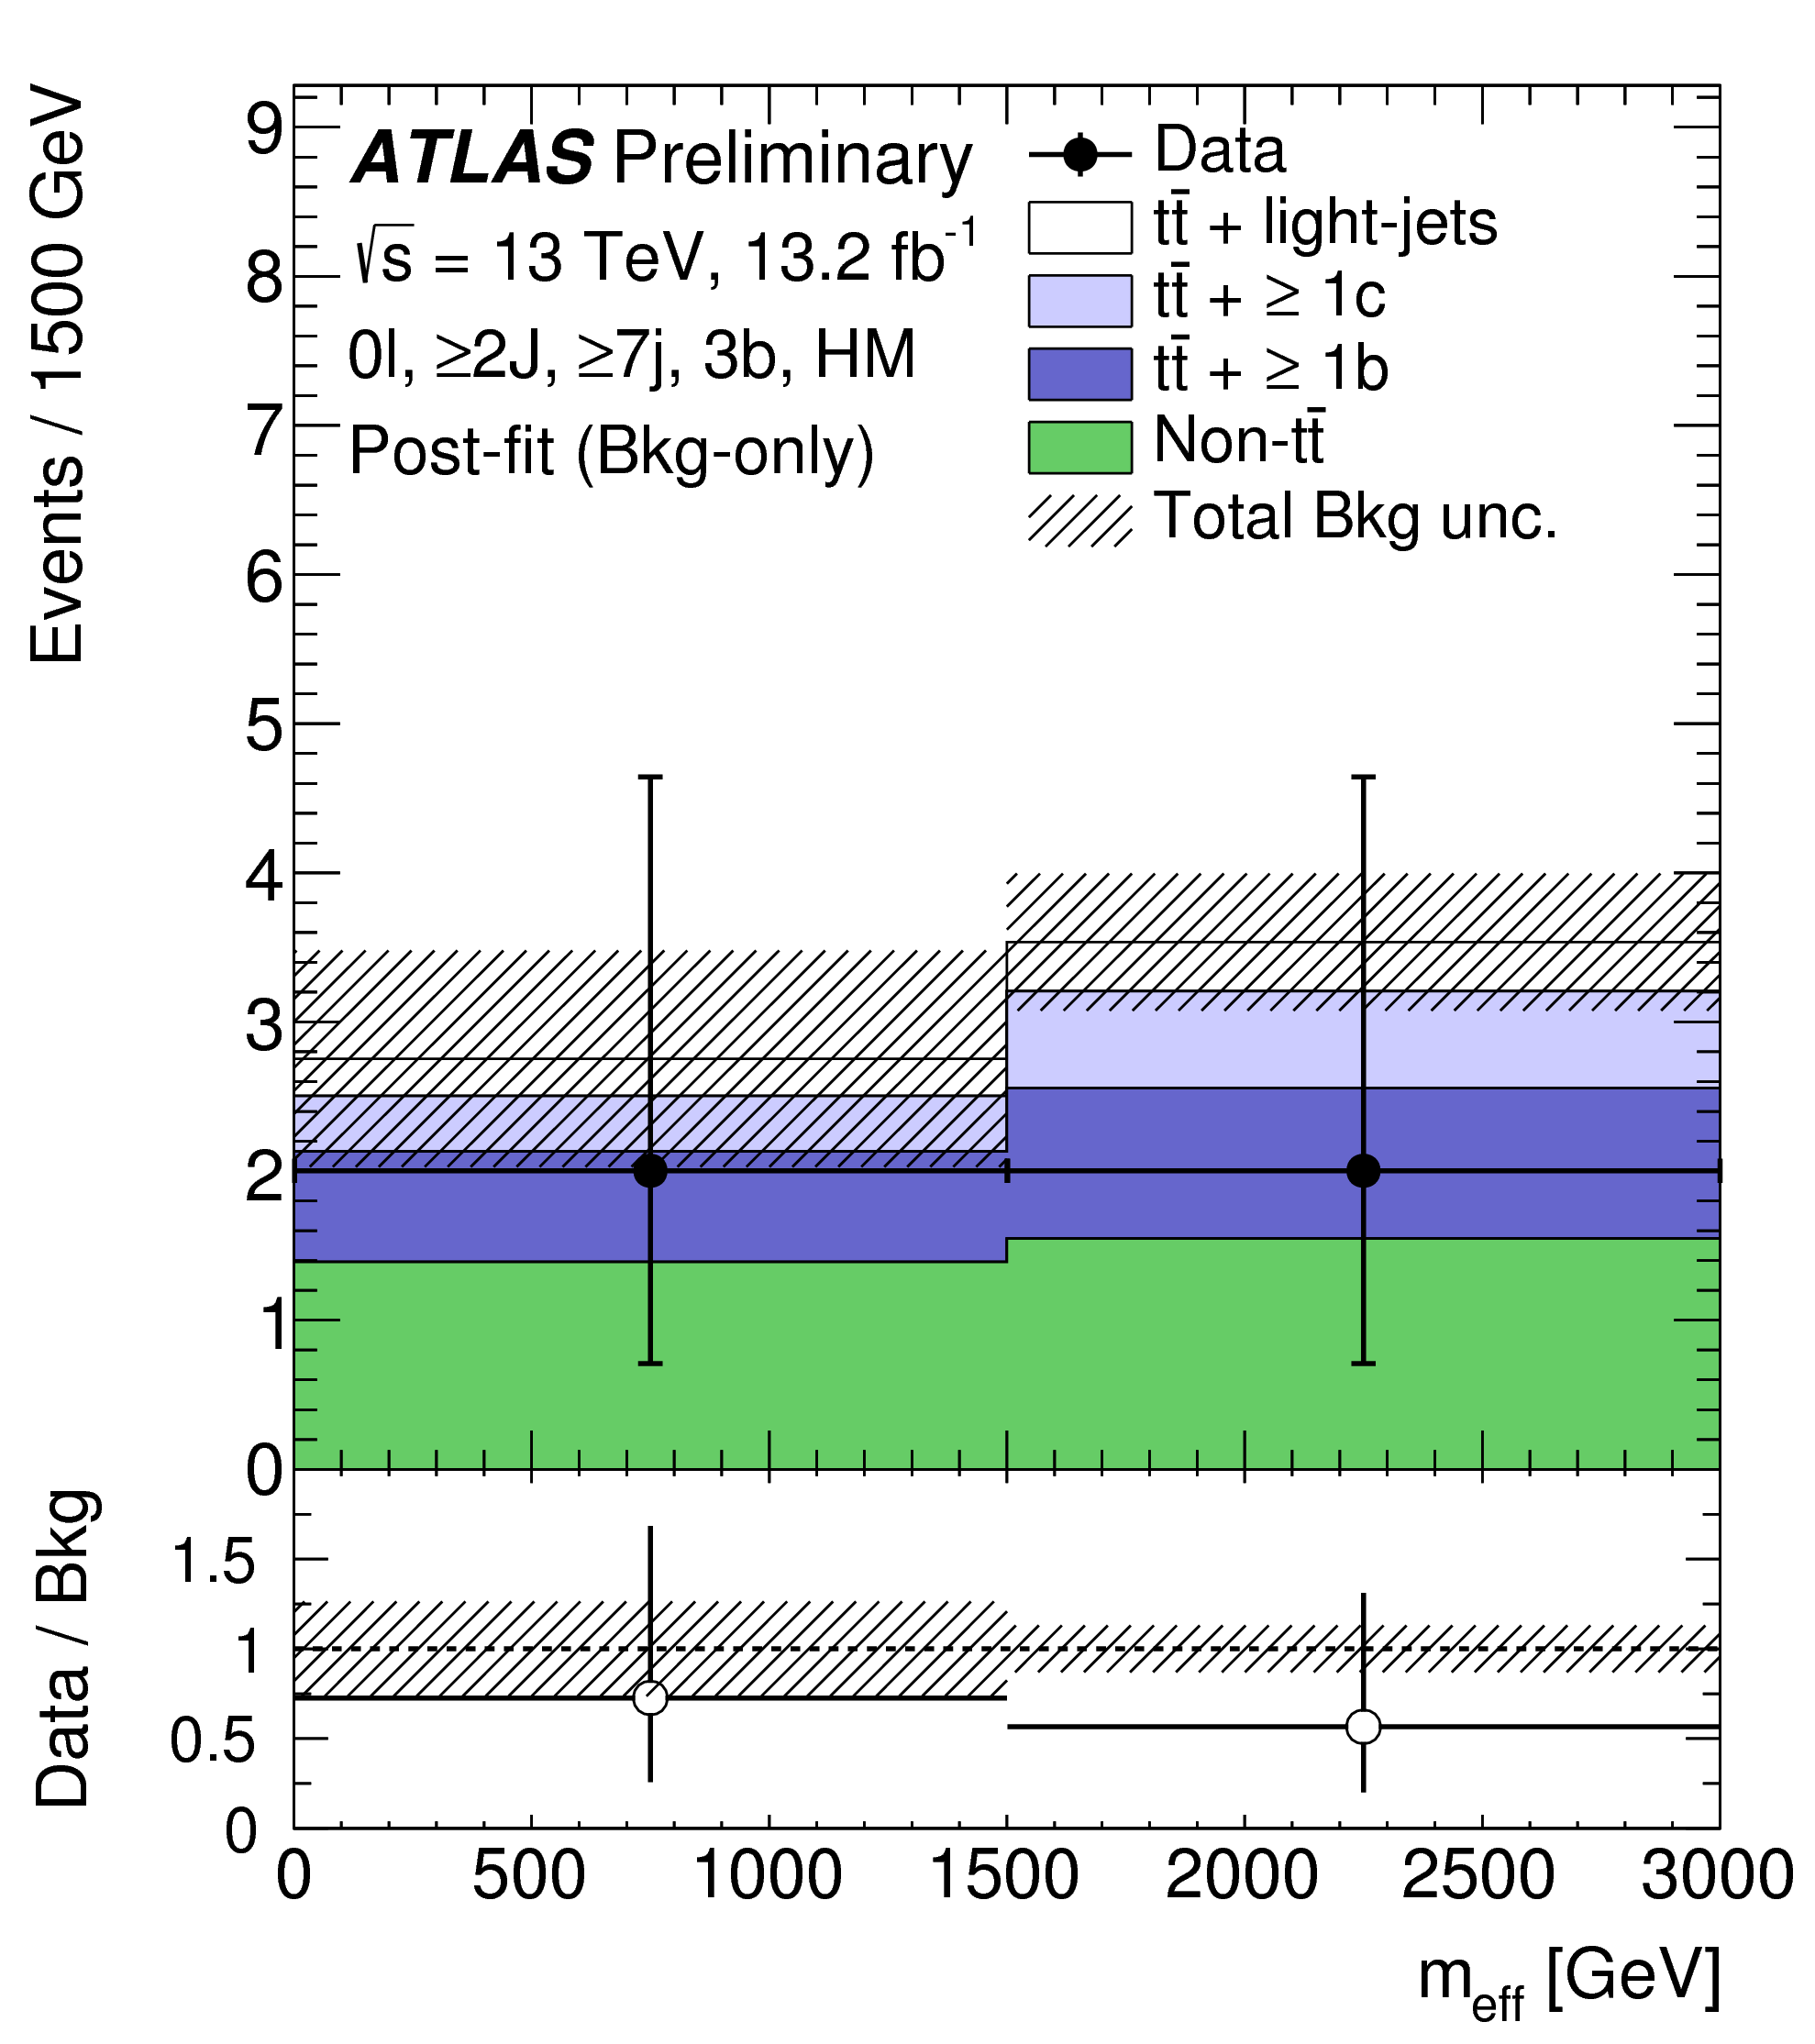
\includegraphics[width=0.9\textwidth]{figures/VLQ/fig_13b.png}
  \caption{}
  \label{}
\end{subfigure}
\begin{subfigure}{0.24\textwidth}
  \centering
  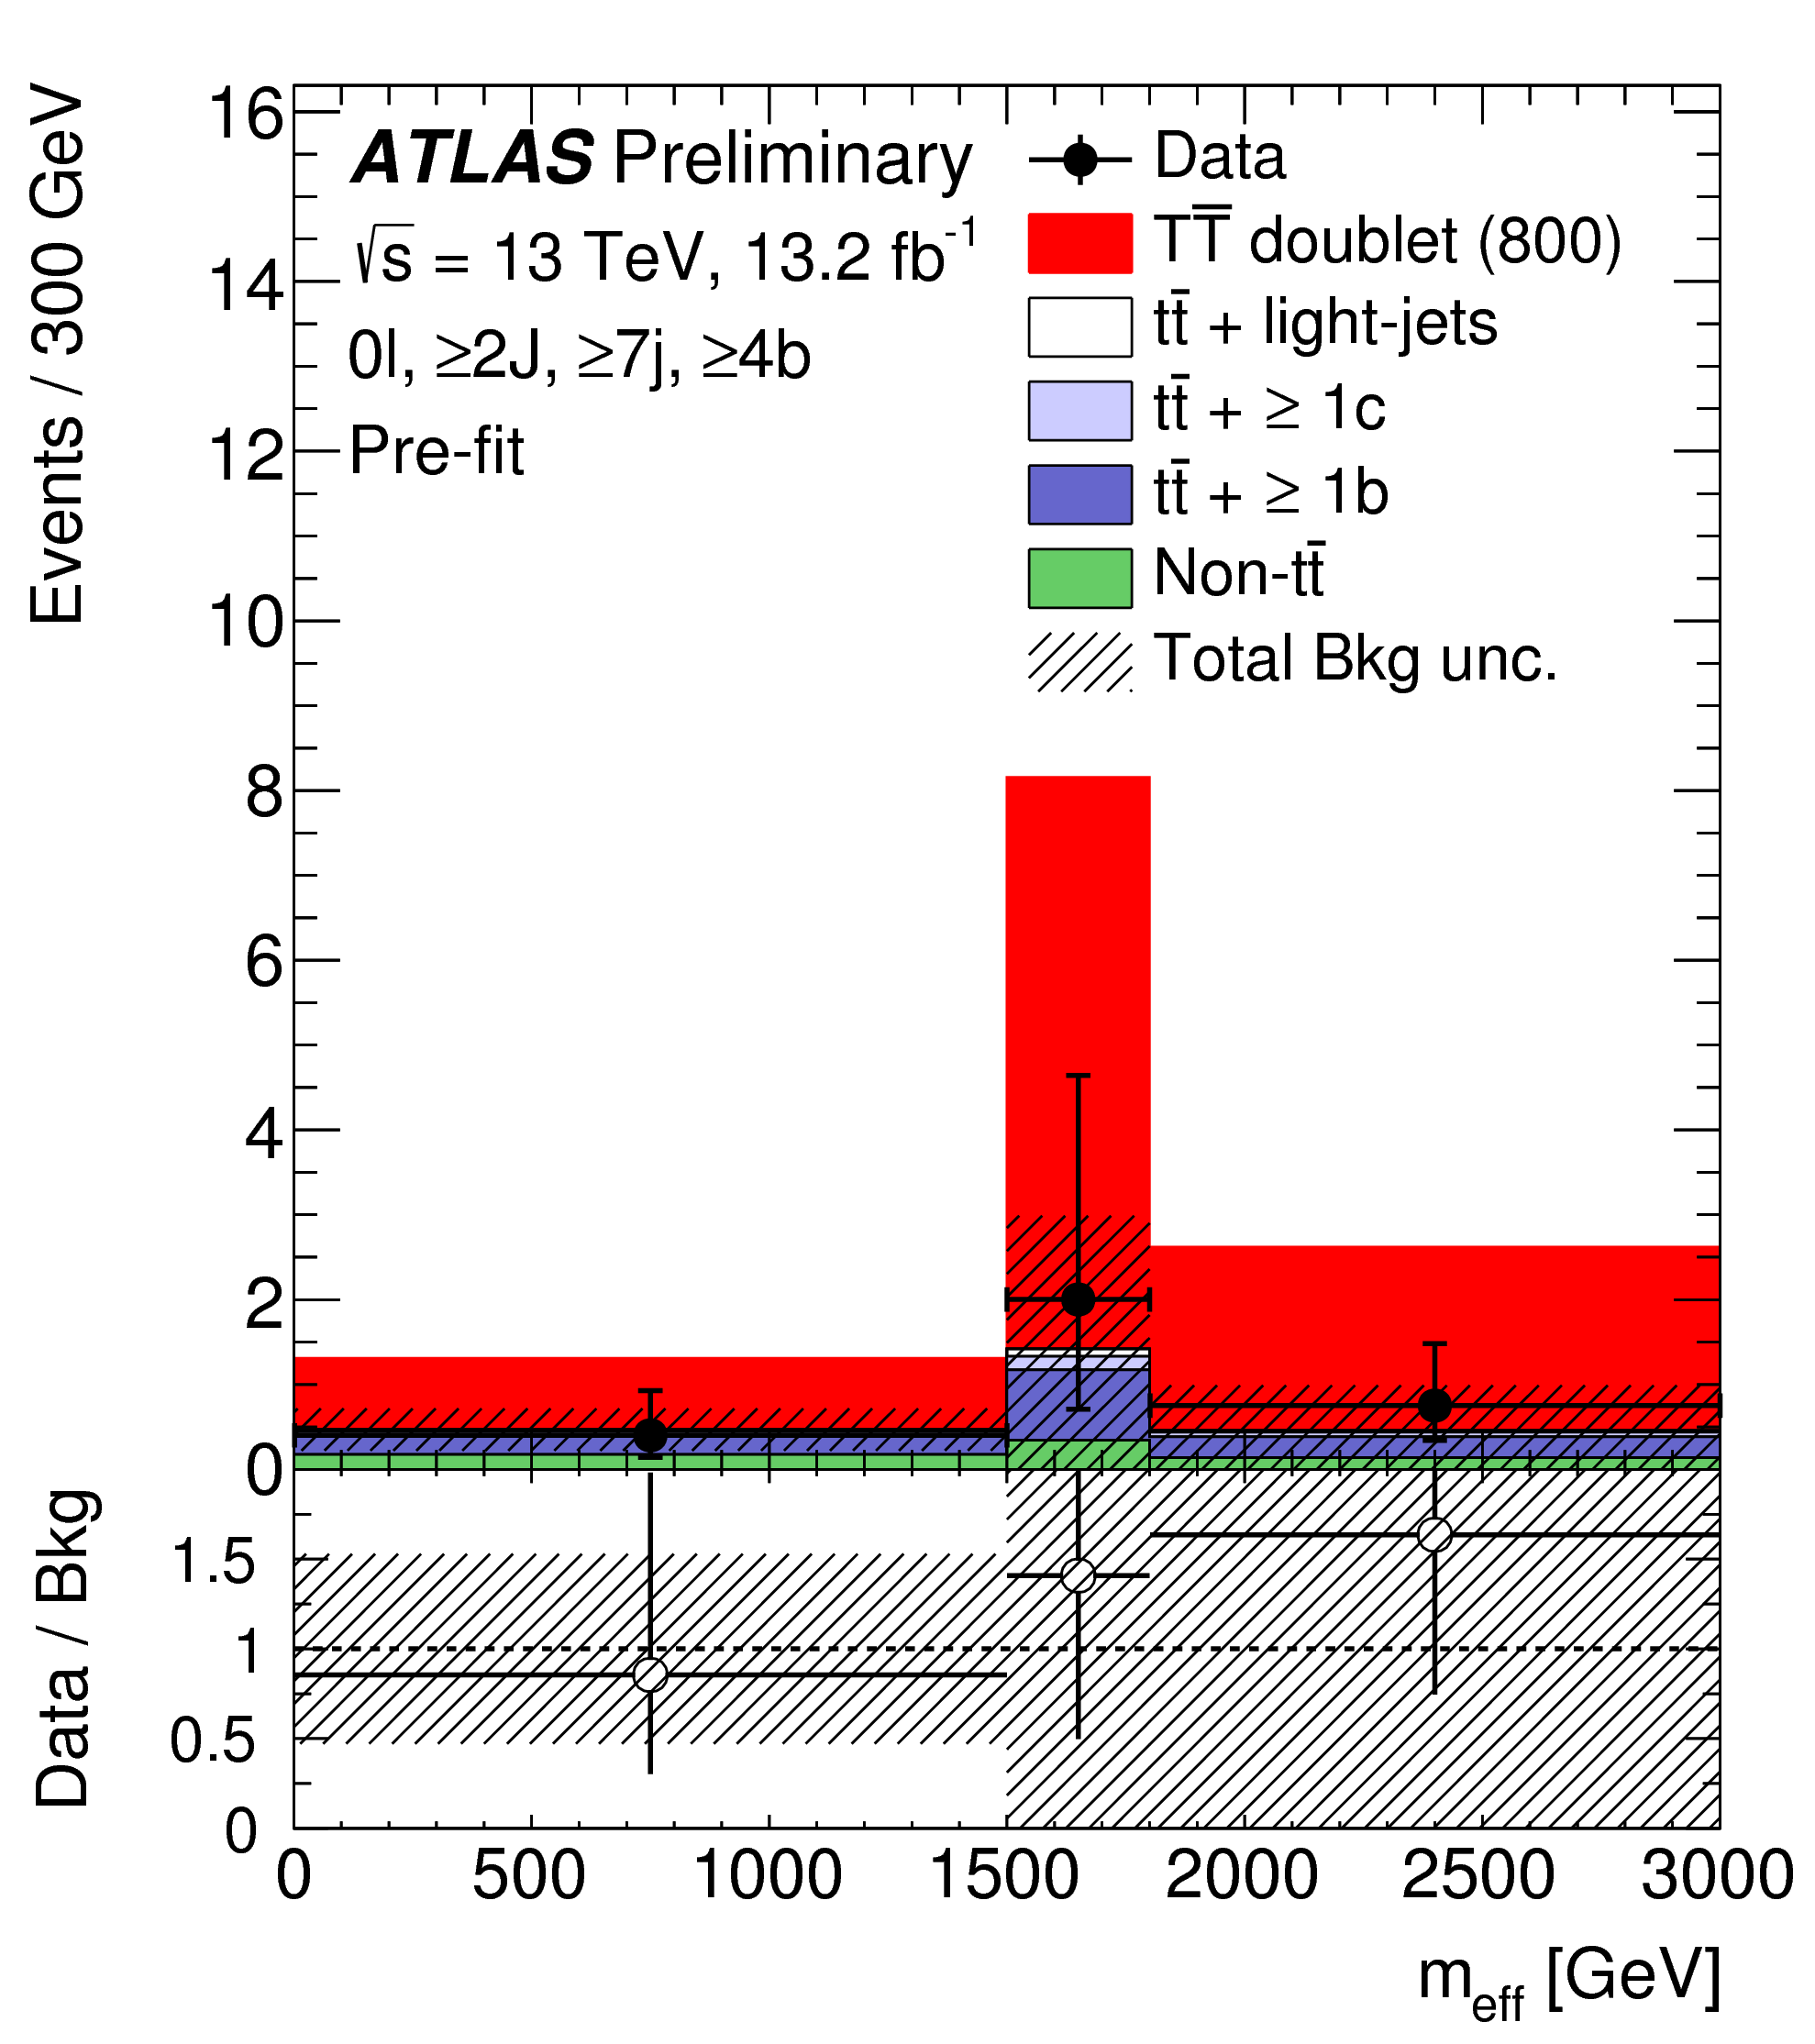
\includegraphics[width=0.9\textwidth]{figures/VLQ/fig_13c.png}
  \caption{}
  \label{}
\end{subfigure}
\begin{subfigure}{0.24\textwidth}
  \centering
  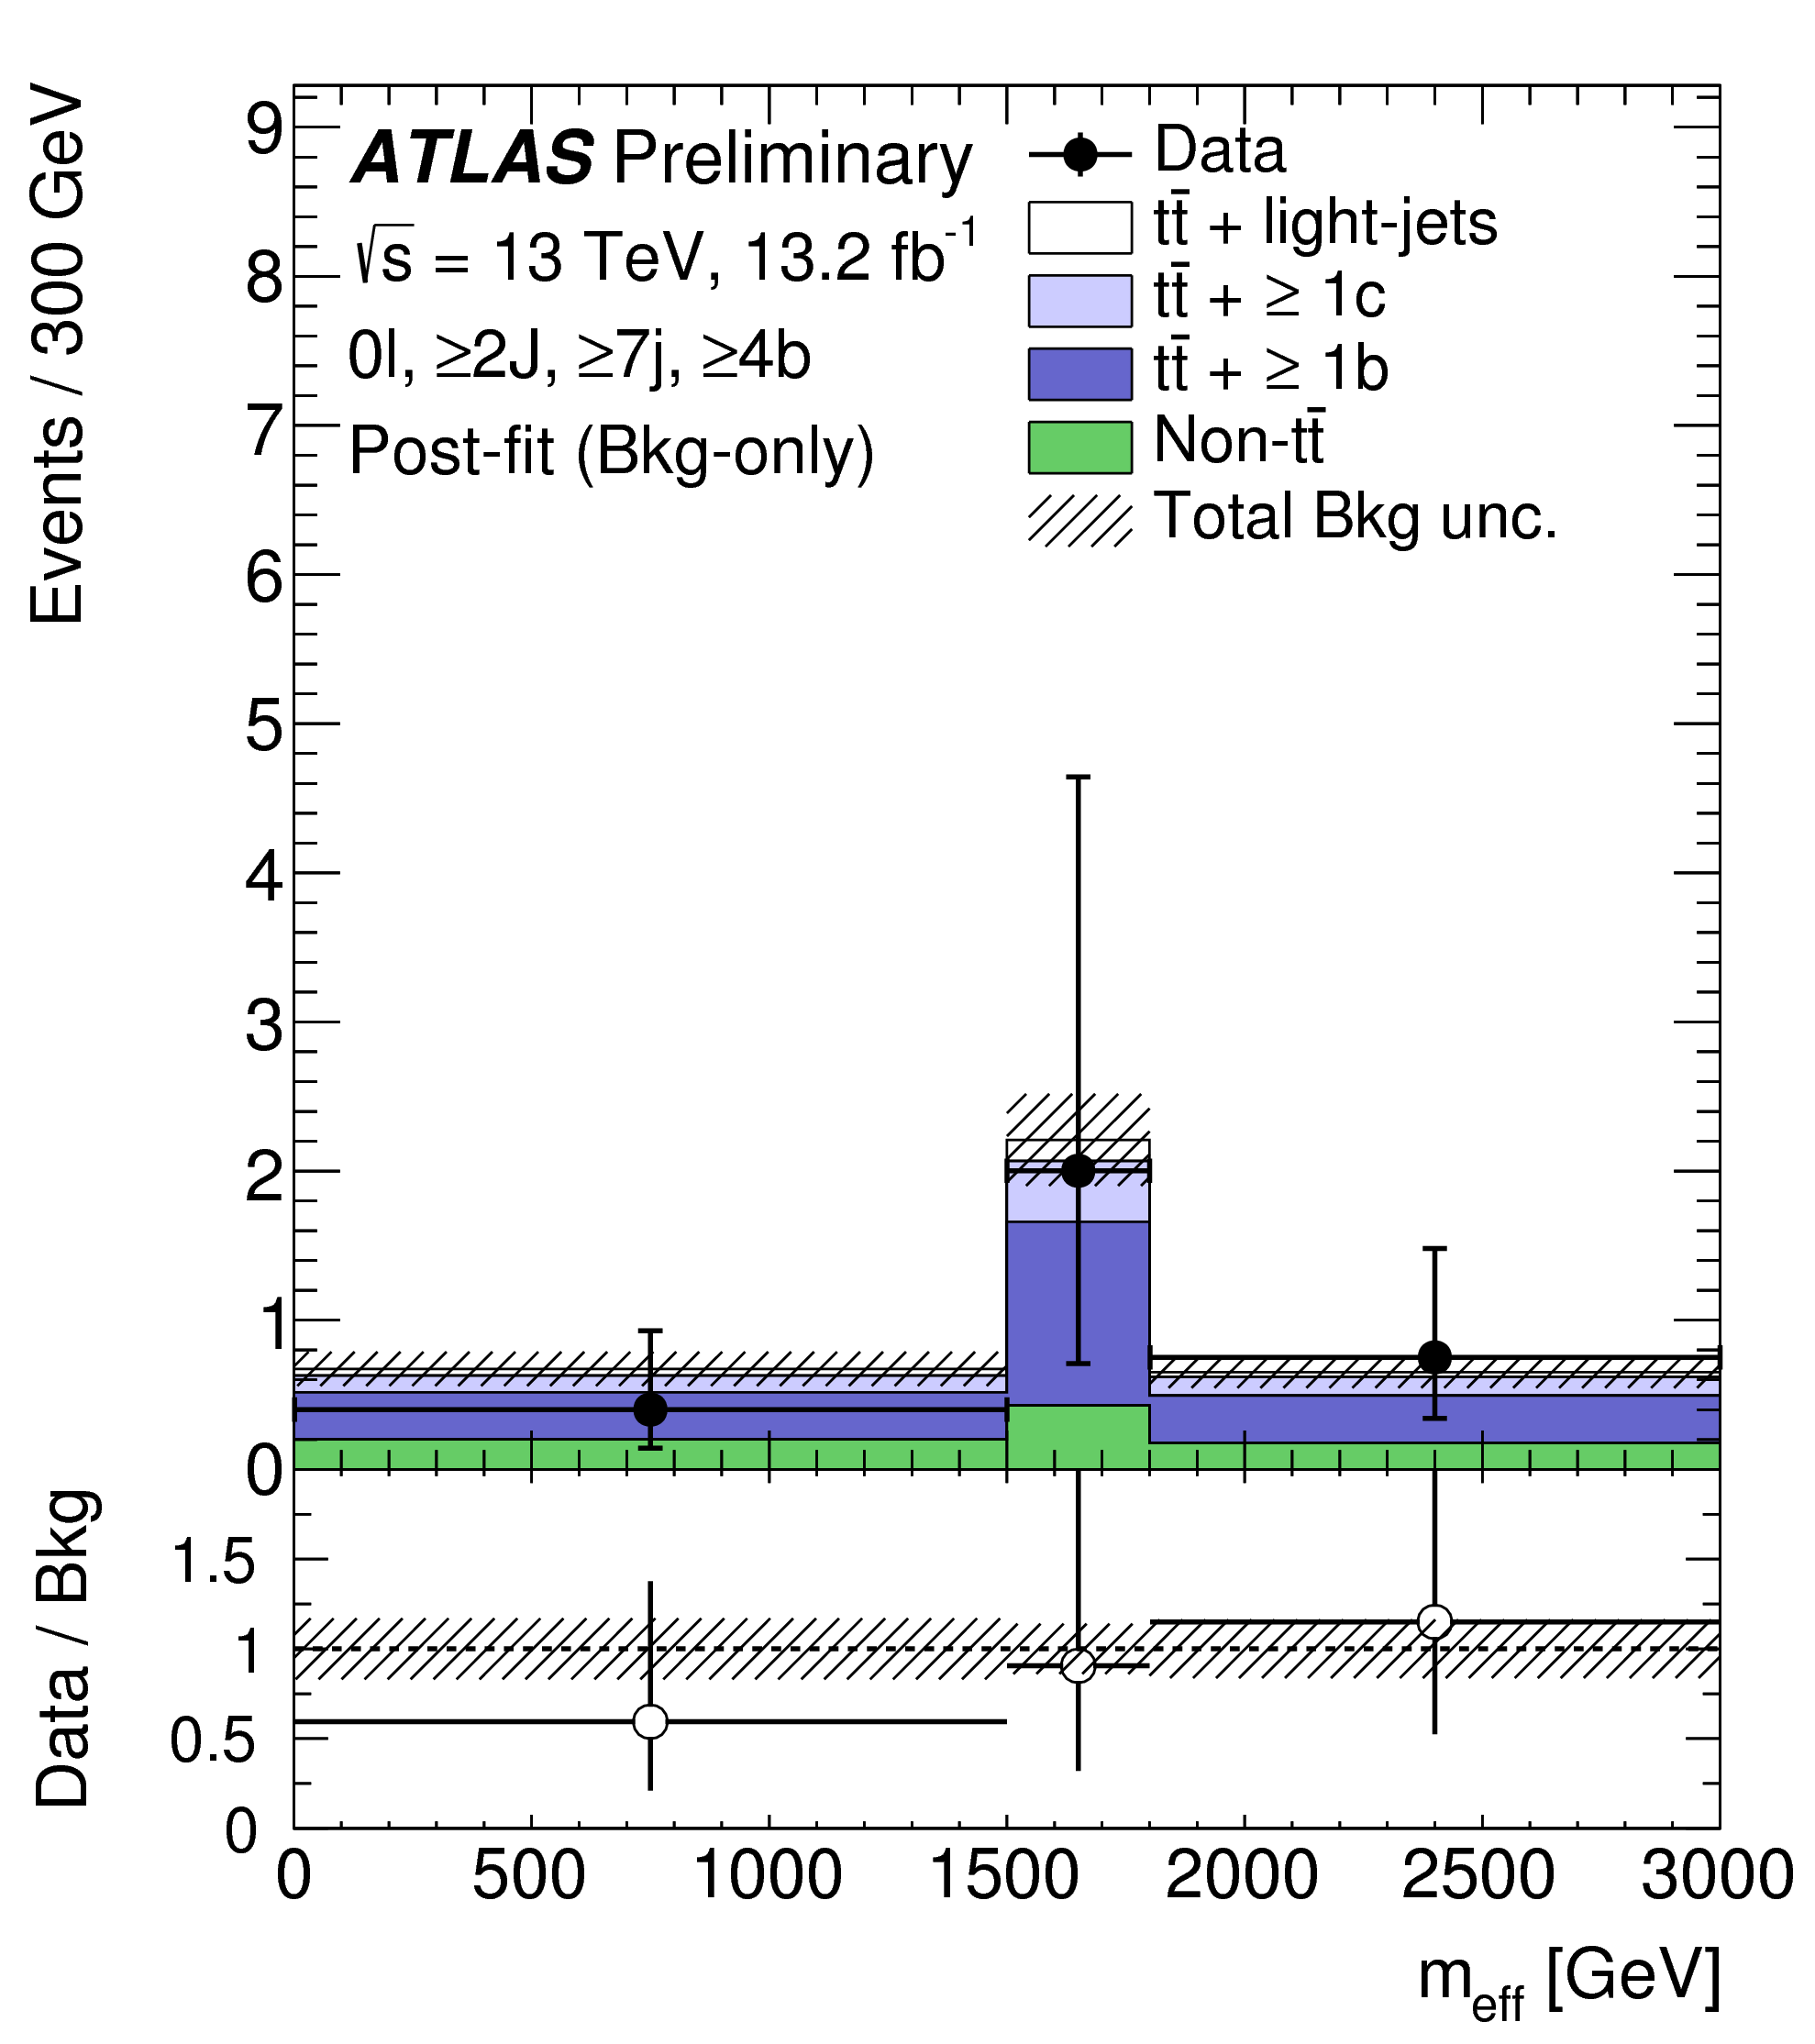
\includegraphics[width=0.9\textwidth]{figures/VLQ/fig_13d.png}
  \caption{}
  \label{}
\end{subfigure}
\captionsetup{width=0.85\textwidth} \caption{\small Comparison between the data and prediction for the $m_{\rm eff}$ distribution in some of the most-sensitive search regions in the 1-lepton channel,
before and after performing the combined fit to data in the 0-lepton and 1-lepton channels (``Pre-fit'' and ``Post-fit'', respectively) under the background-only hypothesis. Shown are the (1J, $\geq$7j, $\geq$4b, HM) region (a) pre-fit and (b) post-fit, the ($\geq$2J, $\geq$7j, $\geq$2b) region (c) pre-fit and (d) post-fit, ($\geq$2J, $\geq$7j, $\geq$3b, HM) region (e) pre-fit and (f) post-fit,  and the ($\geq$2J, $\geq$7j, $\geq$4b) region (g) pre-fit and (h) post-fit.
In the pre-fit figures the expected $T\bar{T}$ signal (solid red) corresponding to $m_{T}=800$ $\gev$ in the doublet $T$-quark scenario is also shown, added on top of the background prediction. The small contributions from $t\bar{t}V$, $t\bar{t} H$, single top, $W/Z$+jets, diboson, and multijet backgrounds are combined into a single background source  referred to as ``Non-$t\bar{t}$''. The last bin in all figures contains the overflow. The bottom panels display the ratios of data to the total background prediction (``Bkg''). The blue triangles indicate points that are outside the vertical range of the figure. The hashed area represents the total uncertainty on the background. In the case of the pre-fit background uncertainty, the normalisation uncertainty on the $t\bar{t}+\ge1b$ background is not included.}
\label{sec:vlq:fig:meff3}
\end{figure}




The large number of events in the signal-depleted regions, together with their different background compositions, and the assumptions of the fit model, allow to constrain the combined effect of several sources of systematic uncertainty. Compared to the pre-fit distributions, the total background uncertainty is significantly reduced after the fit, not only in the background-dominated channels, but also in the signal-rich channels, resulting in an increase in the search sensitivity.\par
The reduced uncertainty results from the significant constraints on some systematic uncertainties, as well as the anti-correlations among sources of systematic uncertainty resulting from the fit to the data. A good agreement is found between data and prediction in all channels. The good performance of the fit can further be validated through comparison between data and total prediction in the validation regions. Pre-fit and post-fit distributions for validation regions can be found in figure \ref{sec:vlq:fig:VR}. The agreement for those regions not used in the fit is also improved after the fit, giving confidence in the overall procedure. 


\begin{figure}[p!]
\begin{subfigure}{0.5\textwidth}
  \centering
  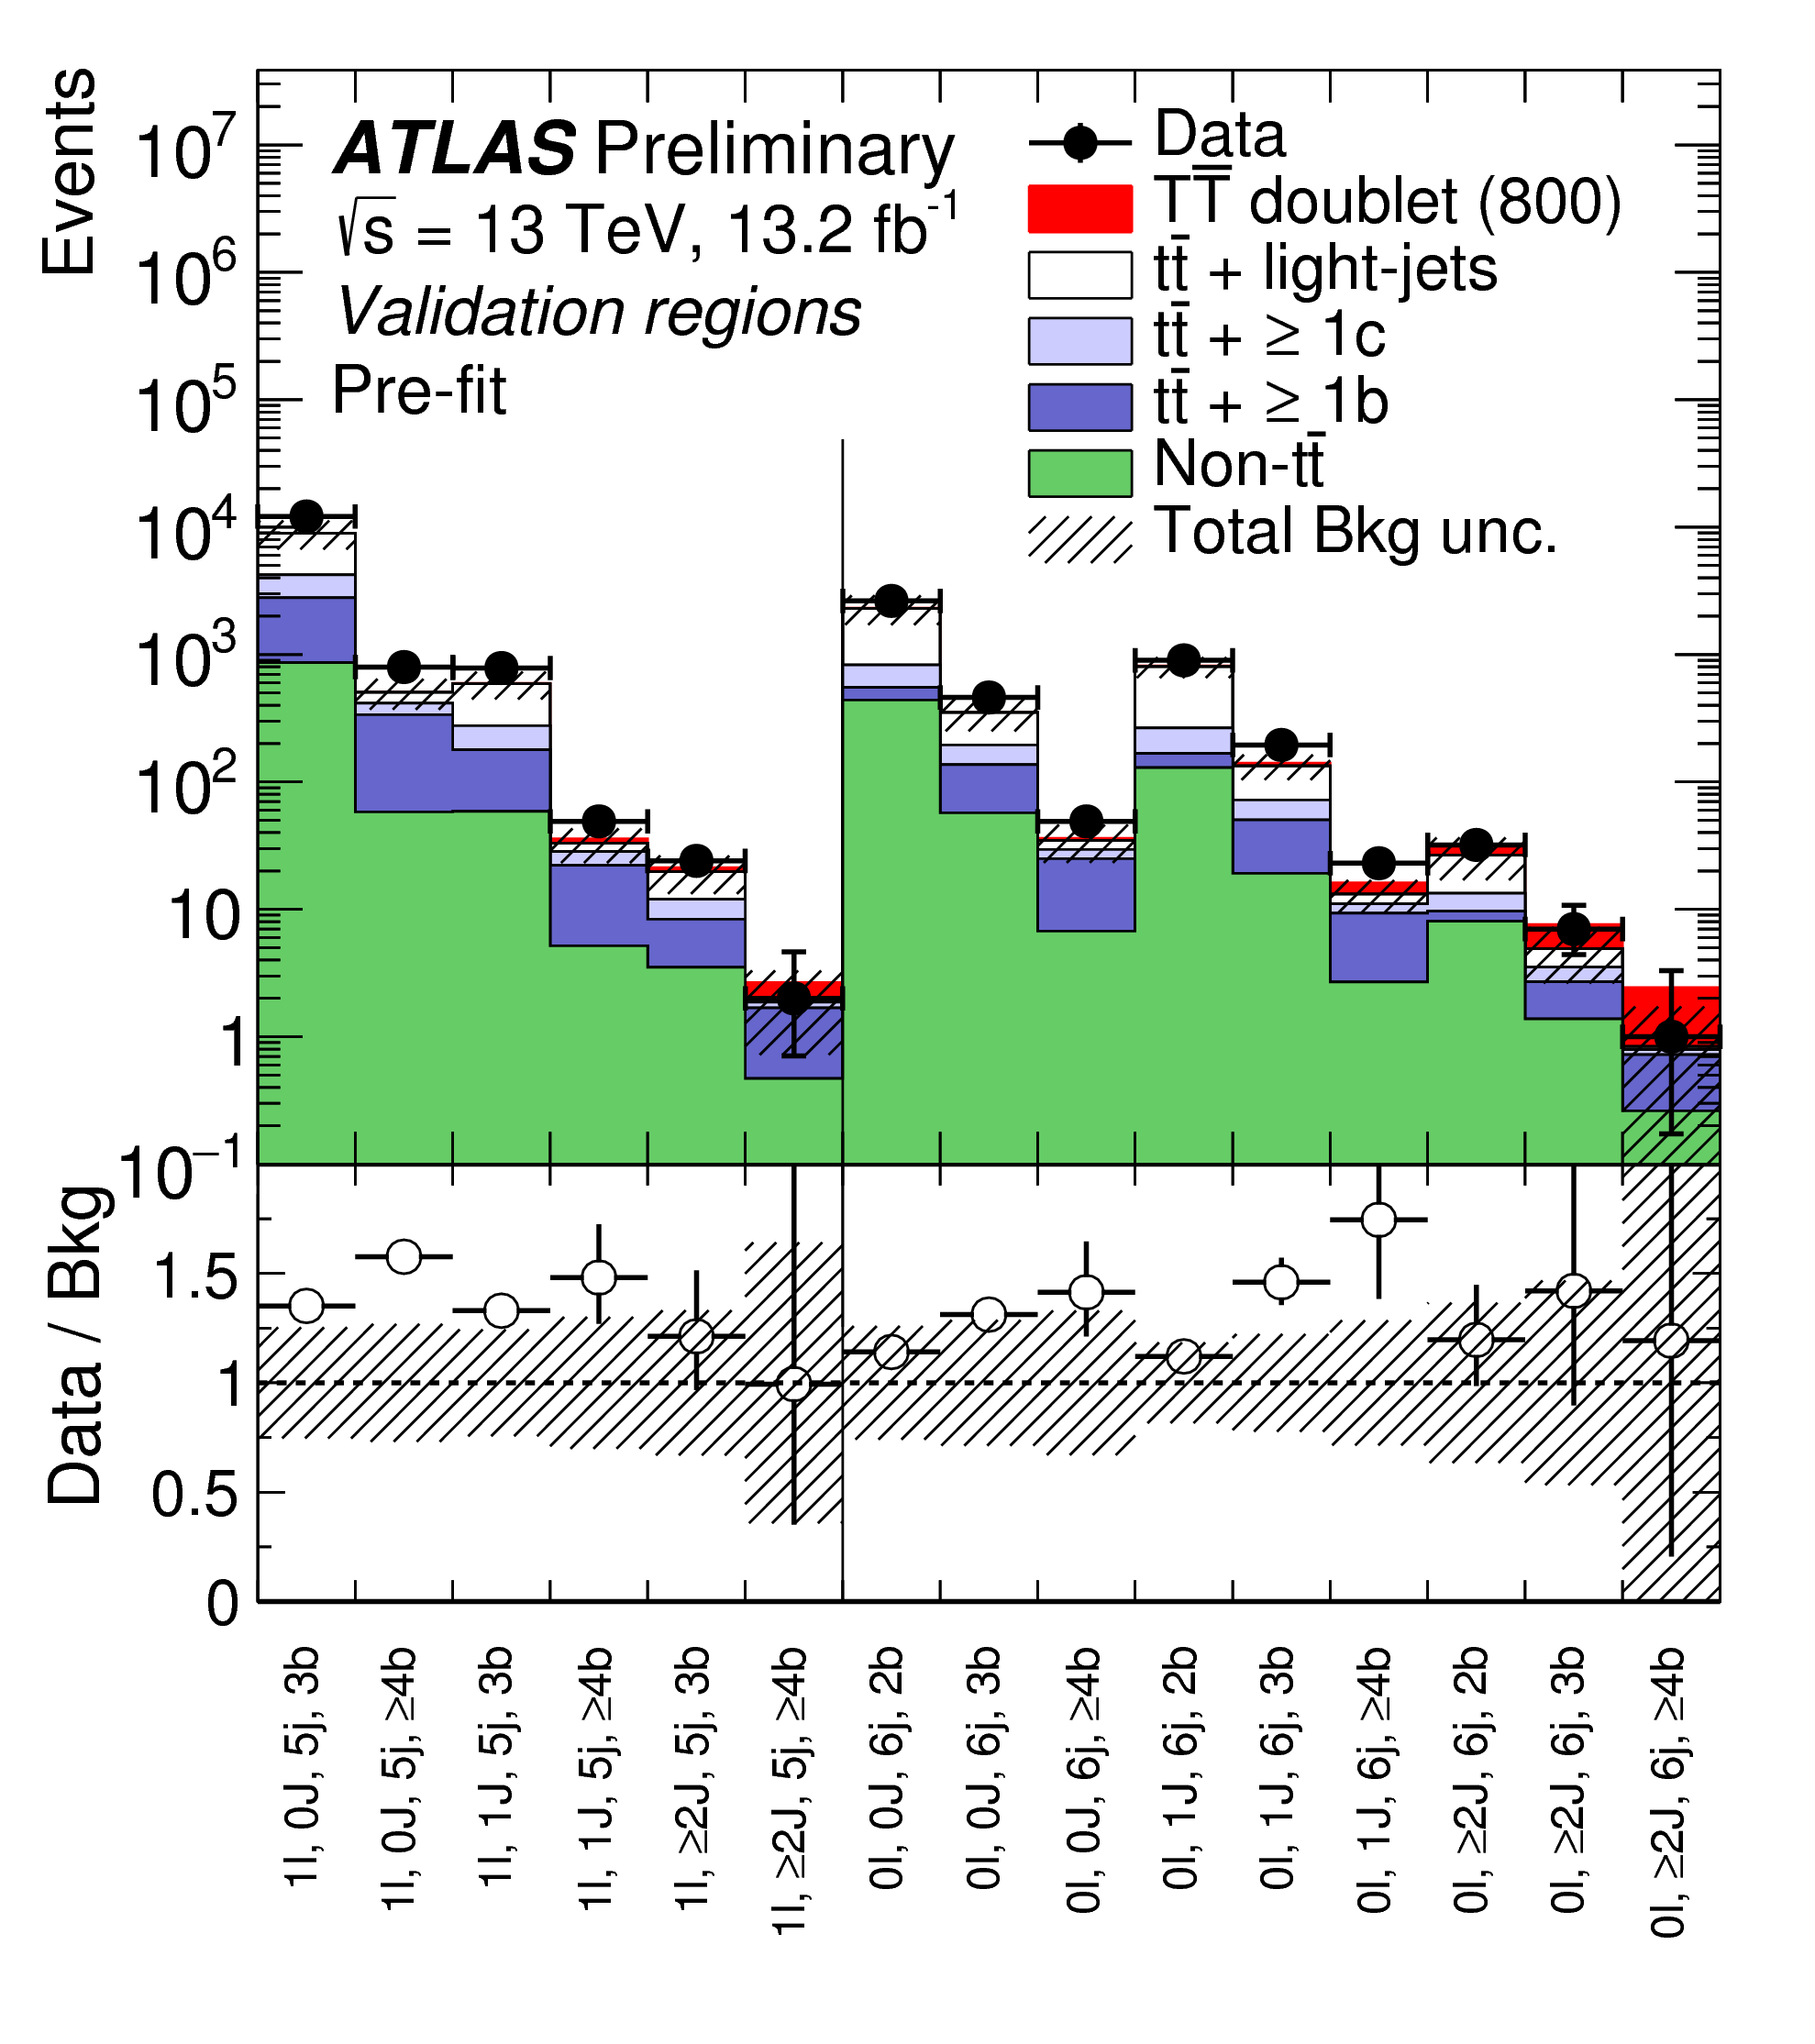
\includegraphics[width=0.9\textwidth]{figures/VLQ/fig_14a.png}
  \caption{}
  \label{}
\end{subfigure}
\begin{subfigure}{0.5\textwidth}
  \centering
  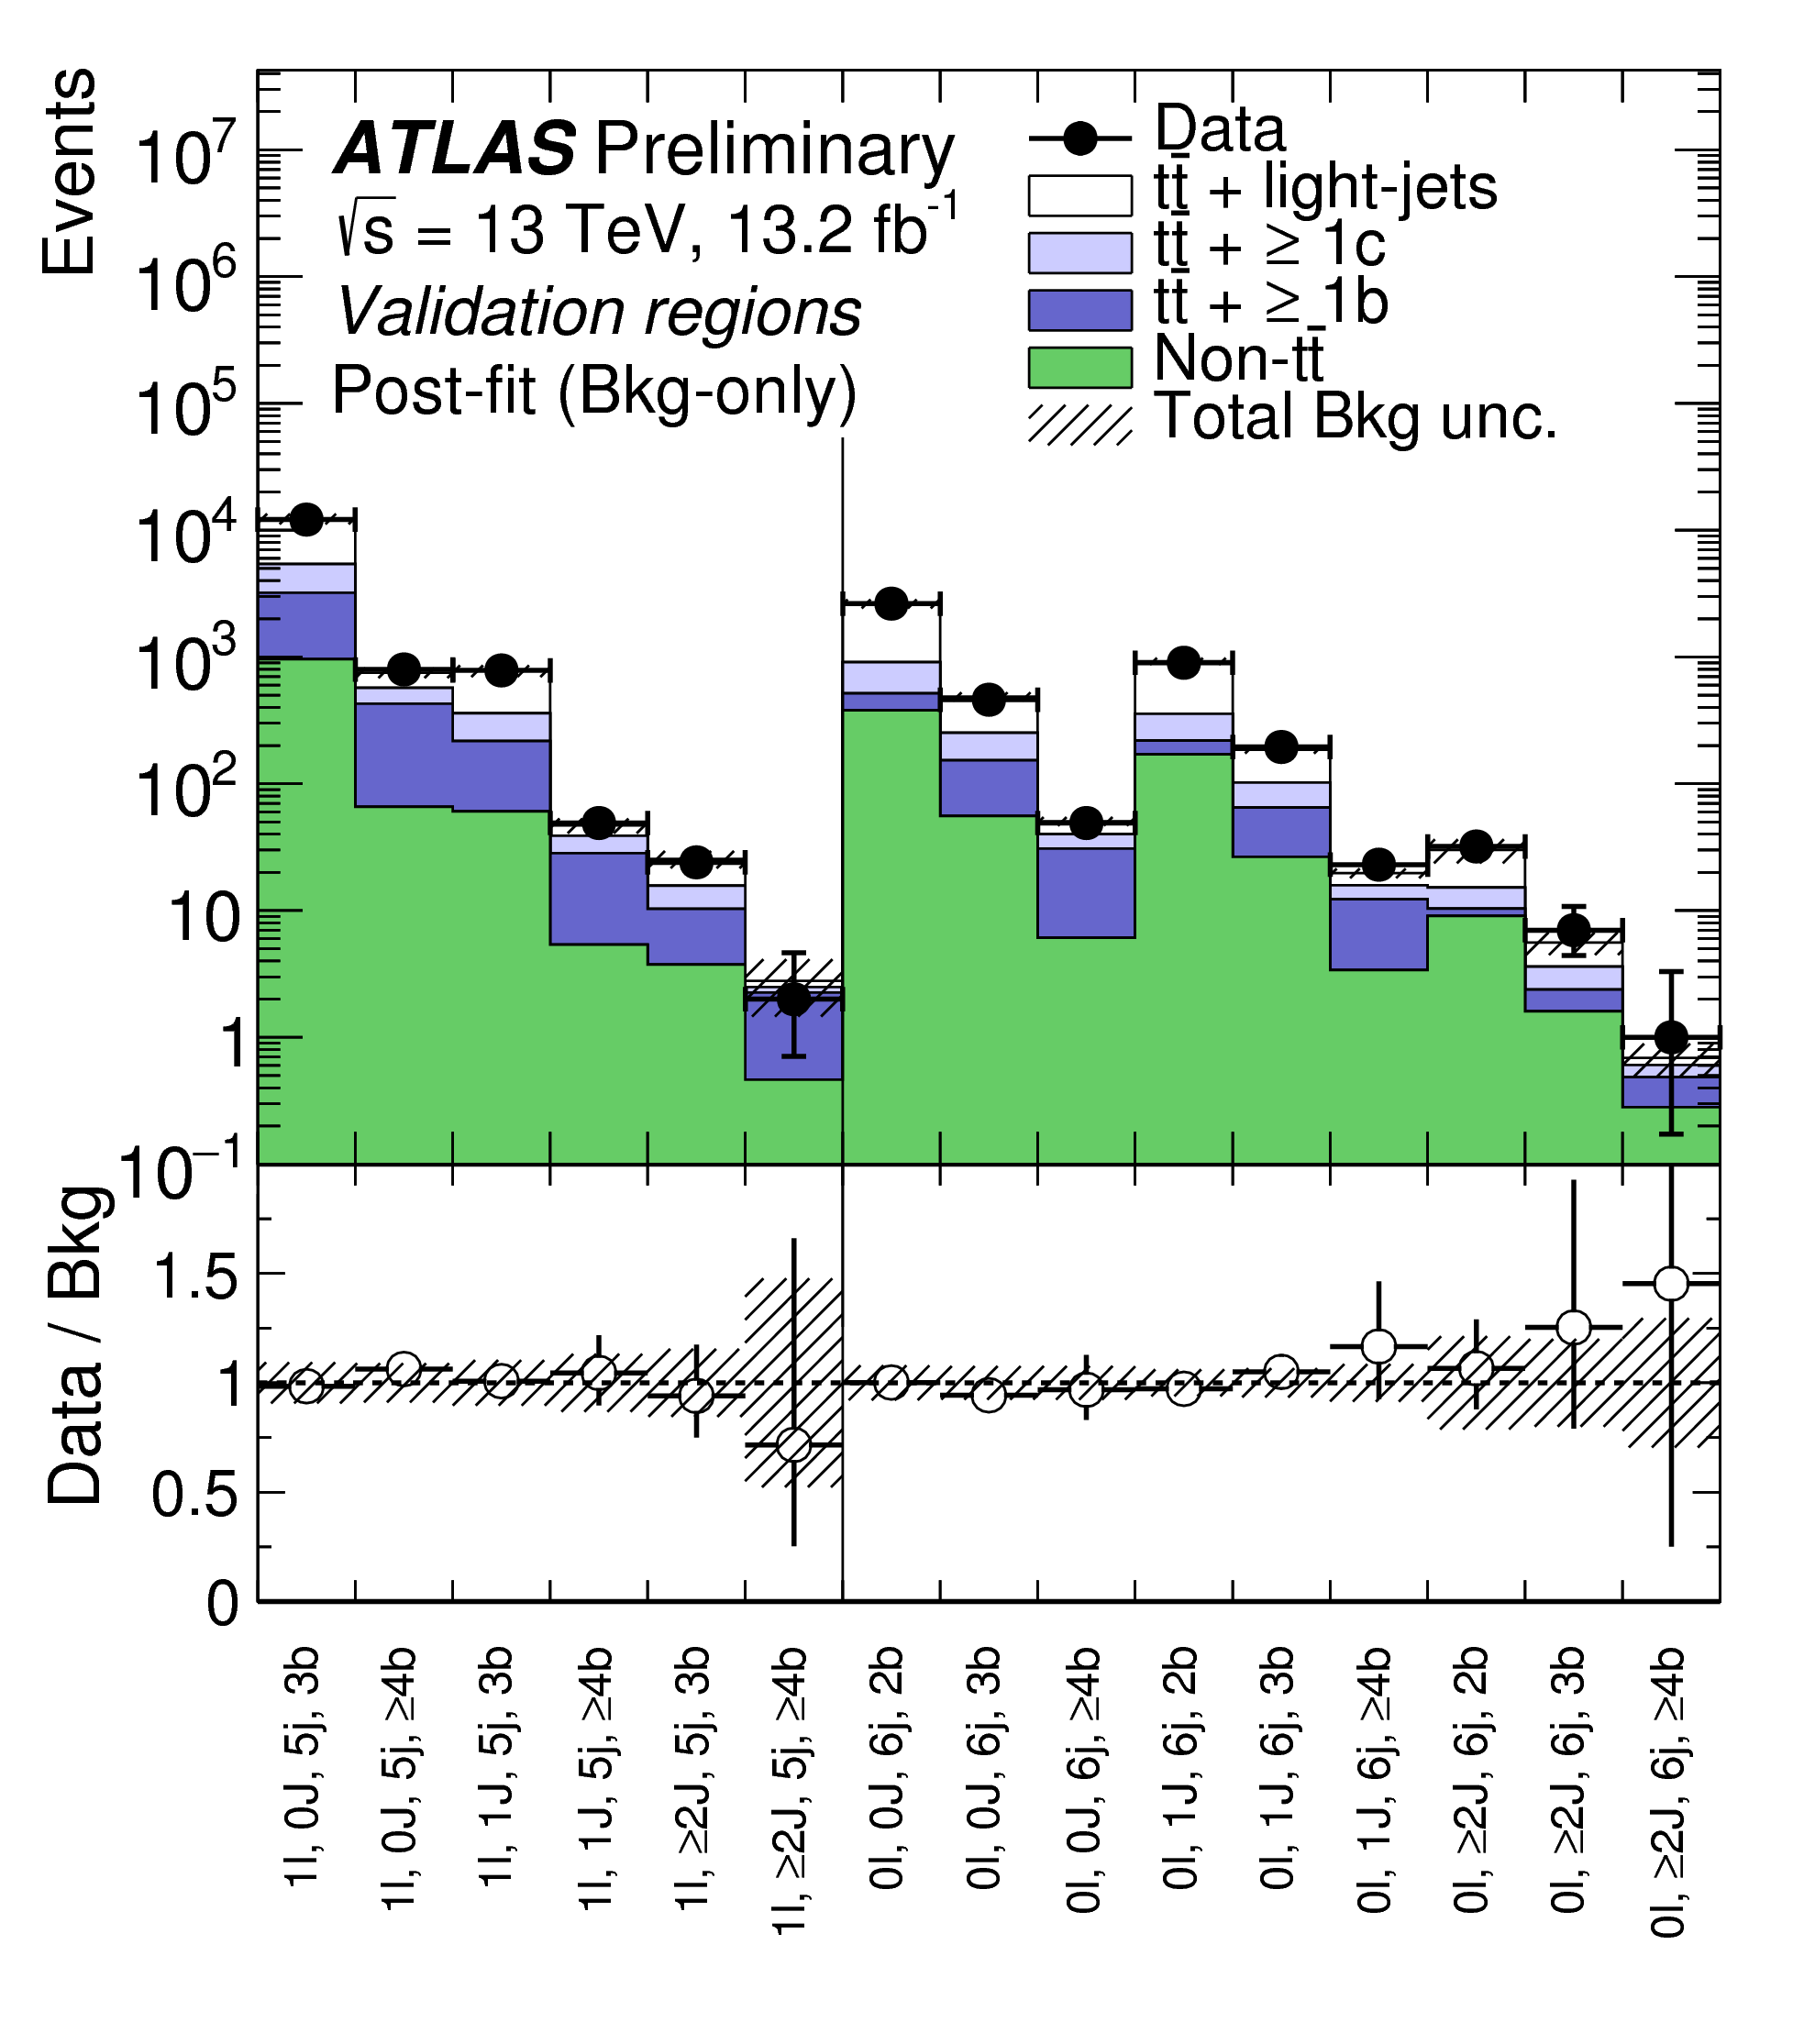
\includegraphics[width=0.9\textwidth]{figures/VLQ/fig_14b.png}
  \caption{}
  \label{}
\end{subfigure}
\captionsetup{width=0.85\textwidth} \caption{\small Comparison between the data and background prediction for the yields in each of the validation regions considered in the 1-lepton and 0-lepton channels (a) before the fit (``Pre-fit'') and (b) after the fit (``Post-fit''). The fit is performed on the data in 1-lepton and 0-lepton channels under the background-only hypothesis considering only the search regions. In the pre-fit figure the expected $T\bar{T}$ signal (solid red) corresponding to $m_{T}=800$ $\gev$ in the doublet $T$-quark scenario is also shown, added on top of the background prediction. The small contributions from $t\bar{t}V$, $t\bar{t} H$, single top, $W/Z$+jets, diboson, and multijet backgrounds are combined into a single background source  referred to as ``Non-$t\bar{t}$''. The last bin in all figures contains the overflow. The bottom panels display the ratios of data to the total background prediction (``Bkg''). The blue triangles indicate points that are outside the vertical range of the figure. The hashed area represents the total uncertainty on the background. In the case of the pre-fit background uncertainty, the normalisation uncertainty on the $t\bar{t}+\ge1b$ background is not included.}
\label{sec:vlq:fig:VR}
\end{figure}


The observed constraints on the systematic uncertainties (i.e. the post-fit error on the NPs) are compatible with the expected values from the Asimov fit (see figure \ref{sec:vlq:fig:asimovfit}).  In general, good consistency is found among the fitted NPs in the individual and combined fits. As for the Asimov fit, the higher statistical power of the 1-lepton channel drives the combined fit. Pulls present in the 1-lepton fit are in most cases translated into the combined fit as well; few exceptions are due to an increase of the statistical power in the combination that allows to pull a NP in the combined fit that was not pulled in the individual fits, or a NP being pulled driven by a high-statistics region in the 0-lepton channel.
The most relevant pulls are discussed in the following:
\bi
 \ib The fitted value for the $t\bar{t}+\ge1b$ normalisation parameter is $1.2\pm0.3$, leading to an increase of this background. In addition, the nuisance parameter controlling the $t\bar{t}+\ge1c$ normalisation is adjusted to scale this background by a factor of $1.5\pm0.4$ relative to its nominal prediction. Those two pulls correct the underestimation of $t\bar{t}+$HF where those processes dominates. The former is mostly pulled in the 1-lepton $0$J, $\ge6$j, $\ge4$b region, where there is enough statistics to measure this background in a region that is depleted in signal. The latter is pulled from the interplay of regions with 3 and $\ge$4 $b$-tagged jets and 0 mass-tagged jets in the combined fit.
 
 \ib $b$, $c$- and light-jet tagging: the fitted values of these NP lead to an increased SF for $c$-tag, mistag and at high $\pt$. The NP corresponding to the largest $c$-tagging uncertainty is pulled. The calibration used the SF from Run 1 (based on a different tagger), which might not be suitable for the new MV2c10 tagger, and the large statistics in the 0 mass-tagged jets regions, play a role in the fit's ability to pull this NP. In particular, the interplay of regions with 2 and 3 $b$-tagged jets in $t\bar{t}$+light-jets events is mainly controlled by the tagging of a $c$-jet from a hadronic $W$-boson decay. This feature brings a good potential for a better derivation of the $c$-jets scale factor.\footnote{The determination of the $c$-jet SF in $\ttbar$ events has not been exploited yet by the ATLAS $b$-tagging calibration effort.} The light-tagging eigenvector is pulled by the interplay of regions with different $b$-tag multiplicity. With high statistics of $b$-jets at high $\pt$ is possible as well to improve the NP that controls the extrapolation at high $\pt$.

\ib Jet energy resolution: the pull of this uncertainty comes from the region $0$J, $\ge7$j, $\ge2$b in the 0-lepton channel, where the jet energy resolution uncertainty can significantly affect the shape of $m_{\rm eff}$ distribution at low $\pt$. Given that this uncertainty has no impact on the signal or background predictions in the search regions, this pull is not considered problematic.
 
\ib $t\bar{t}$ modelling: those uncertainties are strongly constrained, as expected from the Asimov fit, specially those with large variations not compatible with data. The constraints on those NPs come from high-statistics regions with 0 mass-tagged jets. Their pulls corrects the slope observed in the $m_{\rm eff}$ distribution, particularly in the signal-depleted regions where the $\ttbar$+light-jets background is dominant.
 
\ib QCD normalisation: this pull arises from bins in the very low tail of the $m_{\rm eff}$ distributions in the 1-lepton regions due to an overestimation of the multijet background. Given the negligible contributionof this background in the signal-enriched regions, this pull is not considered problematic.
\ei


Other systematic uncertainties are not discussed since their pulls and constrains are less significant, and/or they do not affect appreciably the sensitivity of the analysis.

